%the entire chapter is typed and edited. only the mathematica code on p104 needs conversion to octave code
% all footnotes included


\باب{غیر تابع وقت شروڈنگر مساوات}\شناخت{باب_غیر_تابع_وقت_شروڈنگر_مساوات}
\حصہ{ساکن حالات}
باب اول میں ہم نے تفاعل موج پر بات کی جہاں اس کا استعمال کرتے ہوئے دلچسپی کے مختلف مقداروں کا حساب کیا گیا۔ اب وقت آن پہنچا ہے کہ ہم کسی مخصوص مخفیہ\حاشیہد{بار بار "مخفی توانائی تفاعل" کہنا انسان کو تھکا دیتا ہے، لہٰذا لوگ \عددی{V} کو  صرف "مخفیہ" پکارتے ہیں، اگرچہ ایسا کرنے سے برقی مخفیہ کے ساتھ غلطی پیدا ہو سکتی ہے جو دراصل فی اکائی بار مخفی توانائی ہوتی ہے۔} \عددی{ V (x,t) } کی لئے شروڈنگر مساوات:

\begin{align}\label{مساوات_شروڈنگر_تابع_وقت}
i \hslash \frac{\partial \Psi}{\partial t} = - \frac{\hslash^{2}}{2 m} \frac{\partial^{2} \Psi}{\partial x^{2}} + V\Psi
\end{align}
 حل کرتے ہوئے \عددی{ \Psi (x,t) } حاصل کرنا سیکھیں۔ اس باب میں (بلکہ کتاب کے بیشتر حصے میں) ہم فرض کرتے ہیں کہ \عددی{ V } وقت \عددی{t} کا تابع نہیں ہے۔ ایسی صورت میں  شروڈنگر مساوات  کو \اصطلاح{علیحدگی متغیرات}\فرہنگ{علیحدگی متغیرات}\حاشیہب{separation of variables}\فرہنگ{variables!separation of} کے طریقے سے حل کیا جا سکتا ہے، جو ماہرین طبیعیات کا پسندیدہ طریقہ ہے۔ ہم ایسے حل تلاش کرتے ہیں جنہیں حاصل ضرب:
\begin{align}
\Psi (x,t) = \psi (x) \varphi (t)
\end{align}

 کی صورت میں لکھنا ممکن ہو جہاں \عددی{\psi} صرف \عددی{x} اور \عددی{\varphi} صرف \عددی{t} کا تفاعل ہے۔ بظاہر،  شروڈنگر مساوات کے کسی حل پر ایسی شرط مسلط کرنا درست  نظر نہیں آتا ہے، تاہم  حقیقت میں یوں حاصل کردہ حل بہت کار آمد ثابت ہوتے ہیں۔ مزید (جیسا کہ علیحدگی متغیرات کیلئے عموماً  کیا جاتا ہے) ہم علیحدگی متغیرات سے حاصل شدہ   حلوں   کو یوں آپس میں جوڑ سکتے ہیں کہ ان سے عمومی حل حاصل کرنا ممکن ہو۔ قابل علیحدگی حلوں کیلئے 
\begin{align*}
\frac{\partial \Psi }{\partial t} = \psi \frac{\dif \varphi}{\dif t}, \quad \frac{\partial^{2} \Psi}{\partial x^{2}} = \frac{\dif^{\,2} \Psi}{\dif x^{2}} \varphi
\end{align*}
ہو گا  جو سادہ تفرقی مساوات ہیں۔ ان کی مدد سے شروڈنگر مساوات درج ذیل روپ اختیار کرتی ہے۔
\begin{align*}
i \hslash \psi \frac{\dif \varphi}{\dif t} = - \frac{\hslash^{2}}{2m} \frac{\dif^{\,2} \psi}{\dif x^{2}} \varphi + V\psi\varphi
\end{align*}
دونوں اطراف کو \عددی{\psi\varphi} سے تقسیم کرتے ہیں۔
\begin{align}\label{مساوات_شروڈنگر_علاحدہ_الف}
i\hslash\frac{1}{\varphi} \frac{\dif \varphi}{\dif t} = - \frac{\hslash^{2}}{2m} \frac{1}{\psi} \frac{\dif^{\,2} \psi}{\dif x^{2}} + V
\end{align}
اب بایاں  تفاعل صرف \عددی{t} کا تابع ہے جبکہ دایاں   تفاعل صرف \عددی{x} کا تابع\حاشیہد{دھیان رہے کہ اگر \عددی{V} خود \عددی{x} کے ساتھ ساتھ \عددی{t} کا بھی تفاعل ہوتا تب ایسا ممکن نہ ہوتا۔} ہے۔ یاد رہے اگر \عددی{V} خود \عددی{x} اور \عددی{t} دونوں پر منحصر ہو تب ایسا نہیں ہو گا۔ صرف \عددی{t} تبدیل ہونے سے دایاں تفاعل  کسی صورت تبدیل نہیں ہو سکتا ہے جبکہ بایاں  اور دایاں تفاعل  لازمی طور پر ایک دوسرے کے برابر ہیں،  لہٰذا \عددی{t} تبدیل کرنے سے بایاں تفاعل  بھی تبدیل نہیں ہو گا۔اسی طرح صرف \عددی{x} تبدیل کرنے سے بایاں تفاعل  تبدیل نہیں ہو سکتا ہے اور چونکہ دونوں اطراف لازماً ایک دوسرے کے برابر ہیں لہٰذا \عددی{x} تبدیل کرنے سے دایاں تفاعل بھی تبدیل نہیں ہو گا۔ ہم کہہ سکتے ہیں کہ دونوں اطراف ایک مستقل کے برابر ہوں گے۔ (یہاں تسلی کر لیں کہ آپ کو یہ دلائل سمجھ آ گئے ہیں۔) اس مستقل کو ہم \اصطلاح{ علیحدگی مستقل}\فرہنگ{علیحدگی مستقل}\حاشیہب{separation constant}\فرہنگ{separation constant} کہتے ہیں جس کو ہم   \عددی{E} سے ظاہر کرتے ہیں۔ یوں  مساوات \حوالہ{مساوات_شروڈنگر_علاحدہ_الف}کو 
\begin{align}\label{مساوات_شروڈنگر_علیحدہ_اول}
i\hslash \frac{1}{\varphi} \frac{\dif \varphi}{\dif t} &= E\nonumber\\
\frac{\dif \varphi }{\dif t} &= - \frac{i E}{\hslash} \varphi &&\text{\RL{یا}}
\end{align}
اور
\begin{align}\label{مساوات_شروڈنگر_علیحدہ_دوم}
- \frac{\hslash^{2}}{2m} \frac{1}{\psi} \frac{\dif^{\,2} \psi}{\dif x^{2}} + V &= E\nonumber\\
- \frac{\hslash^{2}}{2m} \frac{\dif^{\,2} \psi}{\dif x^{2}} +V\psi &= E\psi&&\text{\RL{یا}}
\end{align}
لکھا جا سکتا ہے۔ علیحدگی متغیرات نے ایک جزوی تفرقی مساوات کو دو سادہ تفرقی مساوات (مساوات \حوالہ{مساوات_شروڈنگر_علیحدہ_اول} اور \حوالہ{مساوات_شروڈنگر_علیحدہ_دوم}) میں علیحدہ کر دیا۔ ان میں سے پہلی (مساوات \حوالہ{مساوات_شروڈنگر_علیحدہ_اول}) کو حل کرنا بہت آسان ہے: دونوں اطراف کو \عددی{\dif t} سے ضرب دیتے ہوئے   اس کا تکمل لیں۔ یوں 
عمومی حل \عددی{C e^{-iEt/\hslash}} حاصل ہو گا۔ چونکہ ہم حاصل ضرب\عددی{\psi\varphi } میں دلچسپی رکھتے ہیں لہٰذا ہم مستقل \عددی{C} کو \عددی{\psi} میں ضم کر سکتے ہیں۔ یوں مساوات \حوالہ{مساوات_شروڈنگر_علیحدہ_اول} کا حل درج ذیل  ہو گا۔ 
\begin{align}
\varphi(t) = e^{-iEt/\hslash}
\end{align}
دوسری (مساوات \حوالہ{مساوات_شروڈنگر_علیحدہ_دوم}) کو \اصطلاح{غیر تابع وقت شروڈنگر مساوات}\فرہنگ{شروڈنگر!غیر تابع وقت}\حاشیہب{time-independent Schrodinger align}\فرہنگ{Schrodinger!time-independent} کہتے ہیں۔ مخفی توانائی \عددی{V} کو  پوری طرح  جانے بغیر ہم آگے نہیں بڑھ سکتے ہیں۔

اس باب کے باقی حصے میں ہم مختلف سادہ خفی توانائیوں  کیلئے غیر تابع وقت شروڈنگر مساوات حل کریں گے۔ ایسا کرنے سے پہلے آپ پوچھ سکتے ہیں کہ علیحدگی متغیرات میں ایسی  کیا خاص بات ہے؟ بہرحال تابع وقت شروڈنگر مساوات کے زیادہ تر حل \عددی{\psi (x) \varphi (t)} کی صورت میں نہیں لکھے جا سکتے۔ میں اس کے تین جوابات دیتا ہوں۔ ان میں سے دو طبیعی اور ایک ریاضیاتی ہو گا۔ 

\عددی{(1}\quad 
یہ \اصطلاح{ساکن حالات}\فرہنگ{ساکن!حالات}\حاشیہب{stationary states}\فرہنگ{stationary states}  ہیں۔ اگرچہ تفاعل موج خود :
\begin{align}\label{مساوات_شروڈنگر_غیر_تابع_اور_تابع}
\Psi (x,t) = \psi (x) e^{-iEt/\hslash}
\end{align}
وقت \عددی{t} کا تابع ہے لیکن  \ترچھا{کثافت احتمال}:
\begin{align}
\left| \Psi (x,t) \right|^{2} = \Psi^{*}\Psi = \psi^{*}e^{+iEt/\hslash} \psi e^{-iEt/\hslash} = \left| \psi (x) \right|^{2}
\end{align}
وقت کا تابع نہیں ہے؛ تابعیت وقت   مساوات میں سے ختم  ہو  جاتی\حاشیہد{معمول پر لانے کے قابل حل کے لئے لازم ہے کہ \عددی{E} \ترچھا{حقیقی} ہو (سوال \حوالہ{سوال_غیر_تابع_پہلا_سوال}-ا دیکھیں)۔} ہے۔ یہی کچھ کسی بھی حرکی متغیر کی توقعاتی  قیمت  کے حساب  کرنے میں ہو گا۔ مساوات \حوالہ{مساوات_تفاعل_موج_توقعاتی_قیمت_حصول} تخفیف کے بعد درج ذیل صورت اختیار کر لے گی۔ 
\begin{align}\label{مساوات_غیر_تابع_وقت_توقعاتی_قیمت}
\langle Q(x,p) \rangle = \int \psi^{*} Q \left( x, \frac{\hslash}{i} \frac{\dif}{\dif x} \right) \psi \dif x
\end{align}
ہر توقعاتی قیمت \ترچھا{وقت} میں \ترچھا{مستقل} ہو گی؛ ہم \عددی{\varphi (t) } کو نکال  کر   \عددی{\Psi} کی  جگہ \عددی{\psi} استعمال کر کے وہی نتائج حاصل کر سکتے ہیں۔ اگرچہ بعض اوقات \عددی{\psi} کو ہی تفاعل موج پکارا جاتا ہے، لیکن ایسا کرنا حقیقتاً غلط ہے جس سے مسائل پیدا  ہو سکتے ہیں۔ ضروری ہے کہ آپ یاد رکھیں کہ اصل تفاعل موج ہر صورت میں  تابع وقت ہو گا۔ بالخصوص \عددی{ \langle x \rangle } مستقل ہو گا،  لہٰذا (مساوات \حوالہ{مساوات_تفاعل_موج_تعریف_معیار_حرکت} کے تحت) \عددی{ \langle p \rangle = 0 } ہو گا۔ ساکن حال میں کبھی بھی کچھ نہیں ہوتا ۔ 

\عددی{(2} \quad
یہ \ترچھا{غیر مبہم کل توانائی}  سے متعلق حالات ہوں گے۔ کلاسیکی میکانیات میں کل توانائی (حرکی جمع مخفیہ) کو \اصطلاح{ہیملٹنی}\فرہنگ{ہیملٹنی}\حاشیہب{Hamiltonian}\فرہنگ{Hamiltonian} کہتے ہیں جس کو \عددی{H} سے ظاہر کیا جاتا ہے۔ 
\begin{align}
H(x,p) = \frac{p^{2}}{2m} + V(x)
\end{align}
اس کا مطابقتی ہیملٹنی عامل، ضابطے  کے تحت  \عددی{p} کو   \عددی{(\hslash/i)(\partial/\partial x)}  سے تبدیل 
کر  کے  \عددی{(p \rightarrow (\hslash/i)(\partial/\partial x))}،   درج ذیل\حاشیہد{جہاں غلط فہمی پیدا ہونے کی گنجائش ہو وہاں میں عامل پر ٹوپی (\عددی{\hat{}}) کا نشان ڈال کر اس کو اس تغیر پذیر متغیر سے علیحدہ  رکھوں گا جس کو یہ ظاہر کرتا ہو۔ } حاصل ہو گا۔ 
\begin{align}
\hat{H} = - \frac{\hslash^{2}}{2m} \frac{\partial^{2}}{\partial x^{2}} + V(x) 
\end{align}
یوں غیر تابع وقت شروڈنگر مساوات \حوالہ{مساوات_شروڈنگر_علیحدہ_دوم} درج ذیل روپ اختیار کر لے گی 
\begin{align}\label{مساوات_غیر_تابع_شروڈنگر_توانائی_مساوات}
\hat{H} \psi = E\psi
\end{align}

جس کے کل توانائی کی توقعاتی قیمت درج ذیل ہو گی۔ 
\begin{align}
\langle H \rangle = \int \psi^{*} \hat{H}\psi \dif x = E \int \left| \psi \right|^{2} \dif x = E \int \left| \Psi \right|^{2} \dif x = E
\end{align}
آپ دیکھ سکتے ہیں کہ \عددی{\Psi} کی معمول زنی،   \عددی{\psi} کی معمول زنی کے مترادف ہے۔ مزید
\begin{align*}
\hat{H}^{2} \psi = \hat{H} (\hat{H}\psi ) = \hat{H} ( E\psi ) = E (\hat{H} \psi ) = E^{2} \psi 
\end{align*}
کی بنا پر درج ذیل ہو گا۔
\begin{align*}
\langle H^{2} \rangle = \int \psi^{*} \hat{H}^{2} \psi \dif x = E^{2} \int \left| \psi \right|^{2} \dif x = E^{2}
\end{align*}
یوں\عددی{H} کی تغیریت درج ذیل ہو گی۔ 
\begin{align}
\sigma^{2}_{H} = \langle H^{2} \rangle - \langle H \rangle^{2} =E^{2} - E^{2} = 0
\end{align}
یاد رہے کہ \عددی{\sigma = 0} کی صورت میں نمونہ کے  تمام ارکان کی قیمت ایک  جیسی   ہو گی (تقسیم کی توسیع  صفر ہو گ)۔ نتیجتاً قابل علیحدگی حل کی ایک خاصیت یہ ہے کہ کل توانائی کی ہر پیمائش یقیناً  قیمت \عددی{E}  دے گی۔ (اسی    بنا پر ہم نے   علیحدگی مستقل کو \عددی{E} سے ظاہر کیا تھا۔) 

\عددی{(3}\quad
عمومی حل قابل علیحدگی حلوں کا \اصطلاح{خطی جوڑ}\فرہنگ{خطی جوڑ}\حاشیہب{linear combination}\فرہنگ{linear!combination} ہو گا۔ جیسا کہ  ہم جلد دیکھیں گے، غیر تابع وقت شروڈنگر مساوات (مساوات \حوالہ{مساوات_شروڈنگر_علیحدہ_دوم}) لامتناہی تعداد کے حل \عددی{(\psi_{1}(x),\, \psi_{2}(x),\, \psi_{3}(x), \cdots)} دے گی جہاں ہر ایک حل کے ساتھ ایک علیحدگی مستقل \عددی{(E_1,E_2,E_3,\cdots)} منسلک ہو گا لہٰذا ہر \اصطلاح{اجازتی توانائی}\فرہنگ{توانائی!اجازتی}\حاشیہب{allowed energy}\فرہنگ{energy!allowed} کا ایک منفرد تفاعل موج پایا جائے گا۔ 
\begin{align*}
\Psi_{1} (x,t) = \psi_{1}(x)e^{-iE_{1}t/\hslash} , \quad \Psi_{2} (x,t) = \psi_{2}(x)e^{-iE_{2}t/\hslash}, \, \cdots 
\end{align*}
اب (جیسا کہ آپ خود تصدیق کر سکتے ہیں) تابع وقت شروڈنگر مساوات (مساوات \حوالہ{مساوات_شروڈنگر_تابع_وقت}) کی ایک خاصیت یہ ہے کہ اس کے حلوں کا ہر خطی جوڑ\حاشیہد{تفاعلات \عددی{f_1(z)}، \عددی{f_2(z)}، وغیرہ کے خطی جوڑ سے مراد درج ذیل روپ کا فقرہ ہے جہاں \عددی{c_1}، \عددی{c_2}، وغیرہ کوئی بھی (مخلوط) مستقل ہو سکتے ہیں۔
\begin{align*}
f(z)=c_1f_1(z)+c_2f_2(z)+\cdots
\end{align*}
} خود ایک حل ہوتا ہے۔ ایک مرتبہ  قابل علیحدگی حل تلاش کرنے کے بعد ہم زیادہ عمومی حل درج ذیل روپ میں تیار کر سکتے ہیں۔
\begin{align}\label{مساوات_شروڈنگر_خطی_جوڑ_عمومی_حل}
\Psi (x,t) = \sum_{n=1}^{\infty} c_{n} \psi_{n}(x)e^{-iE_{n}t/\hslash}
\end{align}
حقیقتاً تابع وقت شروڈنگر مساوات کا ہر حل درج بالا روپ میں لکھا جا سکتا ہے۔ ایسا کرنے کی خاطر ہمیں وہ مخصوص مستقل   \عددی{(c_{1},\, c_{2}, \, \cdots )} تلاش کرنے ہوں گے جن کو استعمال کرتے ہوئے درج بالا حل (مساوات \حوالہ{مساوات_شروڈنگر_خطی_جوڑ_عمومی_حل}) ابتدائی شرائط  پوری  کرتا ہو۔ آپ آنے والے حصوں میں دیکھیں گے کہ ہم کس طرح یہ سب کچھ کرتے  ہیں۔ باب \حوالہ{باب_قواعد_و_ضوابط} میں ہم اس کو زیادہ مضبوط بنیادوں پر کھڑا کر پائیں گے۔ بنیادی نقطہ یہ ہے کہ ایک  مرتبہ  غیر تابع وقت شروڈنگر مساوات حل کرنے کے بعد آپ کے مسائل ختم ہو جاتے ہیں۔ یہاں سے تابع وقت شروڈنگر مساوات کا عمومی حل حاصل کرنا آسان کام ہے۔ 

گزشتہ چار صفحات میں  بہت کچھ کہا جا چکا ہے۔ میں ان کو مختصراً اور مختلف نقطہ نظر سے دوبارہ پیش کرتا ہوں۔میں آپ کے سامنے ایک عمومی مسئلہ رکھتا ہوں: آپ کو   (غیر تابع وقت)  مخفیہ  \عددی{V(x)} اور ابتدائی تفاعل موج \عددی{\Psi (x,0)} دیے گئے ہوں گے۔ آپ کو مستقبل کے تمام \عددی{t} کیلئے \عددی{ \Psi (x,t)} تلاش کرنا ہو گا۔ ایسا کرنے کی خاطر آپ تابع وقت شروڈنگر مساوات (مساوات \حوالہ{مساوات_شروڈنگر_تابع_وقت}) حل کریں گے۔ پہلا قدم\حاشیہد{بعض اوقات آپ تابع وقت شروڈنگر مساوات کو بغیر علیحدگی متغیرات حل کر  لیتے ہیں (سوال \حوالہ{سوال_غیر_تابع_وقت_بعد_لمبائی} اور سوال \حوالہ{سوال_غیر_تابع_حرکت_پذیر_کنواں} دیکھیں)۔ تاہم ایسی صورتیں بہت کم پائی جاتی ہیں۔} یہ ہو گا کہ  آپ غیر تابع وقت شروڈنگر مساوات (مساوات \حوالہ{مساوات_شروڈنگر_علیحدہ_دوم}) حل کر کے لا متناہی تعداد کے حلوں کا سلسلہ \عددی{(\psi_{1}(x),\, \psi_{2}(x),\, \psi_{3}(x), \cdots)} حاصل کریں گے جہاں ہر ایک
 کی منفرد توانائی \عددی{(E_{1}, \, E_{2}, \, E_{3}, \, \cdots)} ہو گی۔تفاعل  \عددی{\Psi (x,0)}تیار کرنے کی خاطر آپ ان حلوں کا خطی جوڑ لیں گے۔
\begin{align}\label{مساوات_شروڈنگر_ساکن_حالات_کا_خطی_جوڑ}
\Psi (x,0) = \sum_{n=1}^{\infty} c_{n} \psi_{n}(x)
\end{align}
کمال کی بات یہ ہے کہ کسی بھی ابتدائی حال کے لئے آپ ہر صورت میں  مستقل \عددی{c_{1}, \,c_{2}, \,c_{3}, \cdots} دریافت کر پائیں گے۔ تفاعل موج \عددی{\Psi(x,t)} تیار کرنے کی خاطر آپ ہر جزو کے ساتھ مختص تابعیت وقت \عددی{e^{-iE_nt/\hslash}} چسپاں کریں گے۔ 
\begin{align}\label{مساوات_شروڈنگر_عمومی_حل_مجموعہ}
\Psi (x,t) = \sum_{n=1}^{\infty} c_{n} \psi_{n}(x)e^{-iE_{n}t/\hslash} = \sum_{n=0}^{\infty} c_{n} \Psi_{n} (x,t)
\end{align}
چونکہ قابل علیحدگی حل
\begin{align}\label{مساوات_شروڈنگر_تمام_عمومی_حل}
\Psi_{n} (x,t) = \psi_{n}(x) e^{-iE_{n}t/\hslash}
\end{align}
کے تمام احتمال اور توقعاتی قیمتیں غیر تابع وقت ہوں گی لہٰذا یہ خود ساکن حالات ہوں گے، تا ہم عمومی حل (مساوات \حوالہ{مساوات_شروڈنگر_عمومی_حل_مجموعہ}) یہ خاصیت نہیں رکھتا ؛ انفرادی ساکن حالات کی توانائیوں کے  ایک دوسرے سے مختلف ہونے کی بنا پر  \عددی{\left| \Psi \right|^{2}} کا حساب کرتے ہوئے قوت نمائی ایک دوسرے کو حذف نہیں کرتے۔ 


\ابتدا{مثال}\شناخت{مثال_غیر_تابع_دو_ساکن_حالات_ذرہ}
فرض کریں ایک ذرہ کے  ابتدائی حال کو  دو ساکن حالات کے خطی جوڑ   سے ظاہر کیا گیا ہے: 
\begin{align*}
\Psi (x,0) = c_{1} \psi_{1}(x) + c_{2} \psi_{2}(x) 
\end{align*}
(چیزوں کو سادہ رکھنے کی خاطر میں فرض کرتا ہوں کے مستقل \عددی{c_{n}} اور حالات \عددی{\psi_{n} (x)} حقیقی ہیں۔) مستقبل وقت \عددی{ t}  کیلئے تفاعل موج \عددی{\Psi (x,t)} کیا ہو گا ؟ کثافت احتمال تلاش کریں اور ذرے کی حرکت بیان کریں۔ 

حل:\quad
اس کا پہلا حصہ آسان ہے
\begin{align*}
\Psi (x,t) = c_{1} \psi_{1}(x)e^{-iE_{1}t/\hslash} + c_{2} \psi_{2}(x)e^{-iE_{2}t/\hslash}
\end{align*}
جہاں  \عددی{E_{1}} اور \عددی{E_{2}} بالترتیب تفاعل \عددی{\psi_{1}} اور \عددی{\psi_{2}} کی مطابقتی توانائیاں ہیں۔ یوں \عددی{\abs{\Psi}^2}  درج ذیل ہو گا۔ 
\begin{align*}
\left| \Psi (x,t) \right|^{2} &= \left( c_{1} \psi_{1} e^{iE_{1}t/\hslash} + c_{2} \psi_{2} e^{iE_{2}t/\hslash} \right) \left( c_{1} \psi_{1} e^{-iE_{1}t/\hslash} + c_{2} \psi_{2} e^{-iE_{2}t/\hslash} \right) \\
&= c_{1}^{2} \psi_{1}^{2} + c_{2}^{2} \psi_{2}^{2} + 2c_{1}c_{2}\psi_{1}\psi_{2} \cos [ ( E_{2} - E_{1})t/\hslash]
\end{align*}
(میں نے نتیجہ کی سادہ صورت حاصل کرنے کی خاطر \اصطلاح{کلیہ یولر}\فرہنگ{کلیہ!یولر} \عددی{e^{i\theta}=\cos\theta+i\sin\theta} استعمال\حاشیہب{Euler's formula}\فرہنگ{formula!Euler} کیا۔)  ظاہر ہے کہ   کثافت احتمال زاویائی
 تعدد \عددی{(\tfrac{E_2-E_1}{\hslash})} کے ساتھ  سائن نما ارتعاش پذیر ہے لہٰذا یہ ہرگز ساکن حال نہیں ہو گا۔ لیکن دھیان رہے کہ (ایک دوسرے سے مختلف) تونائیوں کے تفاعل کے خطی جوڑ نے یہ حرکت پیدا کی ہے۔ 
\انتہا{مثال}
%===========================
\ابتدا{سوال}\شناخت{سوال_غیر_تابع_پہلا_سوال}
درج ذیل تین مسائل کا ثبوت پیش کریں۔
\begin{enumerate}[a.]
\item
قابل علیحدگی حلوں کے لئے علیحدگی مستقل \عددی{E} لازماً \ترچھا{حقیقی} ہو گا۔ \ترچھا{اشارہ:} مساوات \حوالہ{مساوات_شروڈنگر_غیر_تابع_اور_تابع} میں \عددی{E} کو \عددی{E_0+i\Gamma} لکھ کر (جہاں \عددی{E} اور \عددی{\Gamma} حقیقی ہیں)، دکھائیں کہ تمام \عددی{t} کے لئے مساوات \حوالہ{مساوات_تفاعل_موج_احتمال_اکائی} اس صورت کارآمد ہو گا جب \عددی{\Gamma} صفر ہو۔ 
\item
غیر تابع وقت تفاعل موج \عددی{\psi(x)} ہر موقع پر حقیقی لیا جا سکتا ہے (جبکہ تفاعل موج \عددی{\Psi(x,t)} لازماً مخلوط ہوتا ہے)۔ اس کا ہرگز یہ مطلب نہیں ہے کہ غیر تابع شروڈنگر مساوات کا ہر حل حقیقی ہو گا؛ بلکہ غیر حقیقی حل پائے جانے کی صورت میں اس حل کو ہمیشہ، ساکن حالات کا (اتنی ہی توانائی کا) خطی جوڑ لکھنا ممکن ہو گا۔ یوں بہتر ہو گا کہ آپ صرف حقیقی \عددی{\psi} ہی استعمال کریں۔ \ترچھا{اشارہ:} اگر کسی مخصوص \عددی{E} کے لئے \عددی{\psi{(x)}} مساوات \حوالہ{مساوات_شروڈنگر_علیحدہ_دوم} کو مطمئن کرتا ہو تب اس کا مخلوط خطی جوڑ بھی اس مساوات کو مطمئن کرے گا اور یوں ان کے خطی جوڑ \عددی{(\psi+\psi^*)} اور \عددی{i(\psi-\psi^*)} بھی اس مساوات کو مطمئن کریں گے۔
\item
اگر \عددی{V(x)} \اصطلاح{جفت تفاعل}\فرہنگ{جفت!تفاعل}\حاشیہب{even function}\فرہنگ{function!even} ہو (یعنی  \عددی{V(-x)=V(x)})   تب \عددی{\psi(x)} کو ہمیشہ جفت یا طاق لیا جا  سکتا ہے۔ \ترچھا{اشارہ:} اگر کسی مخصوص \عددی{E} کے لئے \عددی{\psi{(x)}} مساوات \حوالہ{مساوات_شروڈنگر_علیحدہ_دوم} کو مطمئن کرتا ہو تب \عددی{\psi(-x)} بھی اس مساوات کو مطمئن کرے گا اور یوں ان کے جفت اور طاق خطی جوڑ \عددی{\psi(x)\pm\psi(-x)} بھی اس مساوات کو مطمئن کریں گے۔ 
\end{enumerate}
\انتہا{سوال}
%====================
\ابتدا{سوال}\شناخت{سوال_شروڈنگر_کم_سے_کم_توانائی}
دکھائیں کہ غیر تابع وقت شروڈنگر مساوات کے ہر اس حل کے لئے، جس کو معمول پر لایا جا سکتا ہو، \عددی{E} کی قیمت لازماً \عددی{V(x)} کی کم سے کم قیمت سے زیادہ ہو گی۔ اس کا کلاسیکی مماثل کیا ہو گا؟ \ترچھا{اشارہ:} مساوات \حوالہ{مساوات_شروڈنگر_علیحدہ_دوم} کو درج ذیل روپ میں لکھ کر
\begin{align*}
\frac{\dif^{\,2} \psi}{\dif x^2}=\frac{2m}{\hslash^2}[V(x)-E]\psi
\end{align*}
دکھائیں کہ \عددی{E<V_{\text{کمتر}}} کی صورت میں \عددی{\psi} اور اس کے دو گنّا تفرق کی علامتیں لازماً ایک  جیسی    ہوں گی؛ اب دلیل پیش کریں کہ ایسا تفاعل معمول پر لانے کے قابل نہیں ہو گا۔
\انتہا{سوال}
%====================
%%%%%%%%%%%%%%%%%%%%%
%%%%%%%%%%%%%%%

\حصہ{لامتناہی چوکور کنواں}\شناخت{حصہ_غیر_تابع_وقت_چکور_کنواں}
  فرض کریں
\begin{align}\label{مساوات_شروڈنگر_لامتناہی_چکور}
V(x)=
\begin{cases}
0& 0\le x\le a\\
\infty &\text{\RL{دیگر صورت}}
\end{cases}
\end{align}
 (شکل \حوالہ{شکل_غیر_تابع_لامتناہی_چکور_کنواں_مخفیہ})۔اس مخفیہ میں ایک ذرہ مکمل آزاد ہو گا، ماسوائے دونوں سروں یعنی  \عددی{x=0} اور \عددی{x=a} پر، جہاں ایک لامتناہی قوت اس کو فرار ہونے سے روکتی ہے۔ اس کا کلاسیکی نمونہ  کنویں میں بے رگڑ راستے پر چلتا ہوا  جسم ہو سکتا ہے  جو ہمیشہ کے لئے دیواروں سے ٹکرا کر دائیں سے بائیں اور بائیں سے دائیں حرکت کرتا  ہے؛ دیوار کے ساتھ ٹکراؤ  مکمل  لچکدار ہے۔ (اگرچہ یہ ایک فرضی مخفیہ ہے  لیکن آپ اس کو اہمیت دیں۔  باوجود اس کے کہ یہ  انتہائی سادہ نظر آتا ہے،  یہ بہت ساری معلومات فراہم کرتا ہے۔ ہم اس سے بار بار رجوع کریں گے۔)

\begin{figure}
\centering
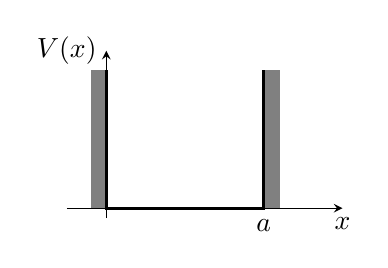
\begin{tikzpicture}
\draw[-stealth](-0.5,0)--(3,0)node[below]{$x$};
\draw[-stealth](0,-0.125)--(0,2)node[left]{$V(x)$};
\fill[gray](0,0) rectangle ++(-0.2,1.75);
\fill[gray](2,0) rectangle ++(0.2,1.75);
\draw[very thick](0,1.75)--(0,0)--(2,0)node[below]{$a$}--(2,1.75);
\end{tikzpicture}
\caption{۔لامتناہی چوکور کنواں مخفیہ (مساوات \حوالہ{مساوات_شروڈنگر_لامتناہی_چکور})}
\label{شکل_غیر_تابع_لامتناہی_چکور_کنواں_مخفیہ}
\end{figure}
کنویں سے باہر \عددی{\psi (x)=0} ہو گا (لہٰذا یہاں ذرے کے پائے جانے کا احتمال صفر ہو گا)۔ کنویں کے اندر، جہاں \عددی{V=0} ہے، غیر تابع وقت شروڈنگر مساوات (مساوات \حوالہ{مساوات_شروڈنگر_علیحدہ_دوم}) درج ذیل روپ اختیار کر لے گی۔
\begin{align}
-\frac{\hslash^{2}}{2m}\frac{\dif^{\,2}\psi}{\dif x^{2}}&=E\psi
\end{align} 
یعنی
\begin{align}\label{مساوات_شروڈنگر_کلاسیکی_ہارمونی_مرتعش}
\frac{\dif^{\,2}\psi}{\dif x^{2}}&=-k^{\,2}\psi, && k\equiv \frac{\sqrt{2mF}}{\hslash}
\end{align}
(اس کو یوں لکھتے ہوئے میں خاموشی سے  \عددی{E\ge 0}  فرض کرتا ہوں۔ ہم سوال \حوالہ{سوال_شروڈنگر_کم_سے_کم_توانائی} سے جان چکے  ہیں کہ \عددی{E< 0 } سے بات نہیں بنے گی۔) مساوات \حوالہ{مساوات_شروڈنگر_کلاسیکی_ہارمونی_مرتعش} کلاسیکی \اصطلاح{سادہ ہارمونی مرتعش}\فرہنگ{ہارمونی!مرتعش}\فرہنگ{مرتعش!ہارمونی}\حاشیہب{simple harmonic oscillator}\فرہنگ{harmonic!oscillator} کی مساوات ہے جس کا عمومی حل درج ذیل  ہے
\begin{align}
\psi(x)=A\sin kx+B\cos kx
\end{align}
 جہاں \عددی{A } اور \عددی{B} اختیاری مستقل ہیں۔ ان مستقلات کو مسئلہ کے \اصطلاح{سرحدی شرائط}\فرہنگ{سرحدی شرائط}\حاشیہب{boundary conditions}\فرہنگ{boundary conditions}متعین کرتے ہیں۔ \عددی{\psi (x)} کے لئے  موزوں سرحدی شرائط کیا ہونگے؟ عموماً \عددی{\psi} اور \عددی{\tfrac{\dif \psi}{\dif x}} \ترچھا{دونوں استمراری} ہونگے، لیکن جہاں مخفیہ لامتناہی کو پہنچتا ہو وہاں صرف اول الذکر کا اطلاق ہو گا۔ (میں حصہ \حوالہ{حصہ_غیر_تابع_ڈیلٹا_تفاعل_مخفیہ}میں ان سرحدی شرائط کو ثابت کروں گا اور \عددی{V=\infty} کی صورتحال کو بھی دیکھوں گا۔ فی الحال مجھ پر یقین کرتے ہوئے میری کہی ہوئی بات مان لیں۔) 

تفاعل \عددی{\psi(x)} کے استمراری شرط کے تحت  درج ذیل ہو گا
\begin{align}
\psi(0)=\psi(a)=0
\end{align} 
تا کہ کنویں کے باہر اور کنویں کے اندر حل ایک  ساتھ جڑ سکیں۔ یہ ہمیں \عددی{A}اور \عددی{B}کے بارے میں کیا معلومات فراہم کرتی ہے؟ چونکہ
\begin{align*}
\psi(0)=A\sin 0+B\cos 0=B
\end{align*}
ہے لہٰذا \عددی{B=0}  پس
\begin{align}
\psi(x)=A\sin kx
\end{align}
ہو گا۔ یوں \عددی{\psi(a)=A\sin ka} کے تحت   \عددی{A=0}  (ایسی صورت میں ہمیں غیر اہم حل \عددی{\psi(x)=0} ملتا ہے جو معمول پر لانے کے قابل نہیں ہے) یا \عددی{\sin ka =0} ہو گا، جس کا نتیجہ   درج ذیل ہو گا۔
\begin{align}
ka&=0,\pm\pi,\pm2\pi,\pm3\pi,\cdots
\end{align} 
اب \عددی{ k =0} بھی \عددی{ \psi(x)=0} دیتا ہے جس  میں ہم دلچسپی نہیں رکھتے اور \عددی{ \sin(-\theta)=-\sin(\theta)} کی بنا پر \عددی{k} کی منفی قیمتیں کوئی نیا حل نہیں دیتی ہیں لہٰذا ہم منفی کی علامت کو \عددی{A} میں ضم کر سکتے ہیں۔ یوں منفرد حل درج ذیل ہوں گے۔ 
\begin{align}
k_{n}=\frac{n\pi}{a},&& n=1,2,3,\cdots
\end{align}

دلچسپ بات یہ ہے کہ \عددی{x=a} پر سرحدی شرط عائد کرنے سے  مستقل \عددی{A} کے بجائے مستقل \عددی{k}متعین ہوتا ہے جس کے نتیجہ میں   \عددی{E} کی اجازتی قیمتیں:
\begin{align}\label{مساوات_شروڈنگر_لامتناہی_چکور_کنواں_توانائیاں}
E_{n}=\frac{\hslash^2 k^{2}_{n}}{2m}=\frac{n^{2}\pi^{2}\hslash^{2}}{2ma^{2}}
\end{align} 
حاصل ہو جائیں گی۔کلاسیکی صورت کے برعکس لامتناہی چوکور کنویں میں کوانٹم ذرہ ہر ایک توانائی کا حامل نہیں ہو سکتا ہے بلکہ اس کی توانائی کی قیمت کو درج بالا مخصوص \اصطلاح{اجازتی}\فرہنگ{اجازتی!قیمتیں}\حاشیہب{allowed}\فرہنگ{allowed!values} قیمتوں\حاشیہد{دھیان رہے کہ غیر تابع وقت شروڈنگر مساوات کو حل کرتے ہوئے سرحدی شرائط عائد  کرنے سے اجازتی توانائیوں کی کوانٹازنی شرط محض تکنیکی وجوہات کی بنا پر  ابھرتا ہے۔} میں سے ہونا ہو گا۔ مستقل \عددی{A} کی قیمت حاصل کرنے کے لئے\عددی{ \psi} کو \ترچھا{معمول پر لانا} ہو گا: 
\begin{align*}
\int_{0}^{a}\abs{A}^{2}\sin^{2}(kx)\dif{x}=\abs{A}^{2}\frac{a}{2}=1,\quad \implies\quad \abs{A}^{2}=\frac{2}{a}
\end{align*} 
یہ صرف  \عددی{A} کی   \ترچھا{مقدار} دیتی ہے ، تاہم مثبت حقیقی جذر \عددی{A=\sqrt{2/a}} منتخب کرنا بہتر ہو گا (کیونکہ \عددی{A} کا زاویہ کوئی طبیعی معنی نہیں رکھتا ہے)۔ اس طرح کنویں کے اندر شروڈنگر مساوات کے حل درج ذیل ہوں گے۔
\begin{align}\label{مساوات_شروڈنگر_میری_سائے}
\psi_{n}(x)=\sqrt{\frac{2}{a}}\sin\big(\frac{n\pi}{a}x\big)
\end{align}

\begin{figure}
\centering
\begin{subfigure}{0.3\textwidth}
\centering
\begin{tikzpicture}
\draw[-stealth](-0.25,0)--(3.25,0)node[below]{$x$};
\draw[-stealth](0,-0.25)--(0,1.25)node[above]{$\psi_1(x)$};
\draw[thick,domain=0:180,smooth,variable=\x] plot ({2.75/180*\x},{sin(1*\x)})node[below]{$a$};
\path(0,0)--(0,-1.1);
\end{tikzpicture}
\end{subfigure}\hfill
\begin{subfigure}{0.3\textwidth}
\centering
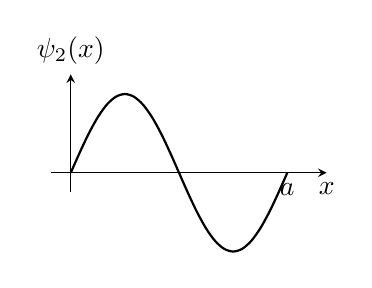
\begin{tikzpicture}
\draw[-stealth](-0.25,0)--(3.25,0)node[below]{$x$};
\draw[-stealth](0,-0.25)--(0,1.25)node[above]{$\psi_2(x)$};
\draw[thick,domain=0:180,smooth,variable=\x] plot ({2.75/180*\x},{sin(2*\x)})node[below]{$a$};
\path(0,0)--(0,-1.1);
\end{tikzpicture}
\end{subfigure}\hfill
\begin{subfigure}{0.3\textwidth}
\centering
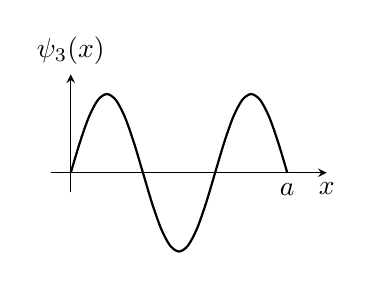
\begin{tikzpicture}
\draw[-stealth](-0.25,0)--(3.25,0)node[below]{$x$};
\draw[-stealth](0,-0.25)--(0,1.25)node[above]{$\psi_3(x)$};
\draw[thick,domain=0:180,smooth,variable=\x] plot ({2.75/180*\x},{sin(3*\x)})node[below]{$a$};
\path(0,0)--(0,-1.1);
\end{tikzpicture}
\end{subfigure}
\caption{لامتناہی چوکور کنویں کے ابتدائی تین ساکن حالات (مساوات \حوالہ{مساوات_شروڈنگر_میری_سائے})۔}
\label{شکل_غیر_تابع_لامتناہی_چکور_تین_ساکن_حالات}
\end{figure}
جیسا کہ وعدہ تھا  (ہر مثبت عدد صحیح \عددی{n} کے عوض ایک حل دے کر) غیر تابع وقت شروڈنگر مساوات نے حلوں کا ایک لامتناہی سلسلہ دیا ہے۔ ان میں سے اولین چند کو شکل \حوالہ{شکل_غیر_تابع_لامتناہی_چکور_تین_ساکن_حالات}میں ترسیم کیا گیا ہے۔ یہ   ایک   دھاگے، جس کی لمبائی \عددی{a} ہو،  پر بننے والی  ساکن امواج کی طرح نظر آتے ہیں ۔ تفاعل \عددی{\psi_{1}} جو \اصطلاح{زمینی حال}\فرہنگ{حال!زمینی}\حاشیہب{ground state}\فرہنگ{state!ground} کہلاتا ہے  کی توانائی کم سے کم ہے۔باقی حالات جن کی توانائیاں \عددی{n^{2}} کے براہ راست بڑھتی ہیں \اصطلاح{ہیجان حالات}\فرہنگ{حال!ہیجان}\حاشیہب{excited states}\فرہنگ{state!excited} کہلاتے ہیں۔ تفاعلات \عددی{\psi_n(x)} چند اہم اور دلچسپ خواص رکھتے ہیں:
\begin{enumerate}[a.]
\item
 کنواں کے وسط کے لحاظ سے یہ تفاعلات باری باری \اصطلاح{جفت}\فرہنگ{جفت} اور \اصطلاح{طاق}\فرہنگ{طاق} ہیں۔ \عددی{\psi_{1}}  جفت ہے، \عددی{\psi_{2}}  طاق ہے، \عددی{\psi_{3}} جفت ہے، وغیرہ وغیرہ۔\حاشیہد{اس تشاکلی کو زیادہ وضاحت سے پیش کرنے کی خاطر بعض مصنفین کنویں کے مرکز کو مبدا پر رکھتے ہیں (یوں کنواں \عددی{-a} تا \عددی{+a} رکھا جاتا ہے)۔ تب جفت تفاعلات کوسائن جبکہ طاق تفاعلات سائن ہوں گے۔ سوال \حوالہ{سوال_غیر_تابع_مبدا_پر_مرکز} دیکھیں۔ }
\item
توانائی بڑھاتے ہوئے ہر اگلے حال کے \اصطلاح{عقدوں}\فرہنگ{عقدہ}\حاشیہب{nodes}\فرہنگ{node} (\اصطلاح{صفر مقام انقطاع}\فرہنگ{صفر مقام انقطاع}\حاشیہب{zero-crossing}\فرہنگ{zero-crossing}) کی تعداد میں ایک \عددی{(1)} کا اضافہ ہو گا۔ (چونکہ سروں پر پائے جانے والے  صفر کو نہیں گنا جاتا ہے لہٰذا) \عددی{\psi_{1}} میں کوئی عقدہ نہیں  ہے، \عددی{\psi_{2}} میں ایک  ہے، \عددی{\psi_{3}} میں دو   پائے جاتے  ہیں، وغیرہ وغیرہ۔
\item
 یہ تمام تفاعل درج ذیل  معنوں میں  باہم  \اصطلاح{عمودی}\فرہنگ{عمودی}\حاشیہب{orthogonal}\فرہنگ{orthogonal} ہیں جہاں  \عددی{m\ne n} ہے۔
\begin{align}
\int\psi_{m}(x)^*\psi_{n}(x)\dif{x}=0
\end{align}
\ترچھا{ثبوت:}\quad
\begin{align*}
\int&\psi_{m}(x)^*\psi_{n}(x)\dif{x}=\frac{2}{a}\int_{0}^{a}\sin\big(\frac{m\pi}{a}x\big)\sin\big(\frac{n\pi}{a}x\big)\dif{x}\\
&=\frac{1}{a}\int_{0}^{a}\big[\cos\big(\frac{m-n}{a}\pi x\big)-\cos\big(\frac{m+n}{a}\pi x\big)\big]\dif{x}\\
&=\big\{\left.\frac{1}{(m-n)\pi}\sin\big(\frac{m-n}{a}\pi x\big)-\frac{1}{(m+n)\pi}\sin\big(\frac{m+n}{a}\pi x\big)\big\}\right\vert_{0}^{a}\\
&=\frac{1}{\pi}\big\{\frac{\sin[(m-n)\pi]}{(m-n)}-\frac{\sin[(m+n)\pi]}{(m+n)}\big\}=0
\end{align*} 
دھیان رہے کہ \عددی{m= n} کی صورت میں درج بالا دلیل درست نہیں ہو گی؛ (کیا آپ بتا سکتے ہیں کہ ایسی صورت میں دلیل کیوں ناقابل قبول ہو گی؟) ایسی صورت میں معمول پر لانے کا عمل اس   تکمل کی قیمت \عددی{1} کر دے گا۔ درحقیقت، عمودیت اور معمول زنی کو ایک فقرے میں سمویا جا سکتا ہے:\حاشیہد{یہاں تمام \عددی{\psi} حقیقی ہیں لہٰذا \عددی{\psi_m} پر \عددی{^*} ڈالنے کی ضرورت نہیں ہے، لیکن مستقبل کی ضرورتوں  کا   لحاظ کرتے ہوئے  ایسا کرنا ایک اچھی عادت ہے۔}
\begin{align}
\int\psi_{m}(x)^*\psi_{n}(x)\dif{x}=\delta_{mn}
\end{align}
جہاں \عددی{\delta_{mn}} \اصطلاح{کرونیکر ڈیلٹا}\فرہنگ{ڈیلٹا!کرونیکر}\حاشیہب{Kronecker delta}\فرہنگ{delta!Kronecker} کہلاتا ہے  جس کی تعریف درج ذیل ہے۔ 
\begin{align}
\delta_{mn}=
\begin{cases}
0& m\neq n\\
1 & m=n
\end{cases}
\end{align} 
ہم کہتے ہیں کہ مذکورہ بالا (تمام) \عددی{\psi} \اصطلاح{معیاری عمودی}\فرہنگ{معیاری عمودی}\فرہنگ{معیاری عمودی}\حاشیہب{orthonormal}\فرہنگ{orthonormal} ہیں۔ 
\item
 یہ \اصطلاح{مکمل}\فرہنگ{مکمل}\حاشیہب{complete}\فرہنگ{complete} ہیں، جس سے مراد ہے کہ کسی بھی دوسرے تفاعل \عددی{f(x)} کو ان کے خطی جوڑ سے بنایا جا سکتا ہے۔
\begin{align}\label{مساوات_شروڈنگر_کوئی_تفاعل}
f(x)=\sum_{n=1}^{\infty}c_{n}\psi_{n}(x)=\sqrt{\frac{2}{a}}\sum_{n=1}^{\infty}c_{n}\sin\big(\frac{n\pi}{a}x\big)
\end{align}
 میں تفاعلات \عددی{\sin\tfrac{n\pi x}{a}} کی مکملیت کو یہاں ثابت نہیں کروں گا، البتہ اگر آپ  اعلٰی علم الاحصاء  سے واقف ہیں تو آپ پہچان سکتے ہیں کہ  مساوات \حوالہ{مساوات_شروڈنگر_کوئی_تفاعل}  اور کچھ نہیں بلکہ  \عددی{f(x)} کا \اصطلاح{فوریئر تسلسل}\فرہنگ{تسلسل!فوریئر}\حاشیہب{Fourier series}\فرہنگ{series!Fourier}ہے۔ یہ حقیقت، کہ ہر تفاعل کو فوریئر تسلسل کی صورت میں پھیلا کر لکھا جا سکتا ہے، بعض اوقات \اصطلاح{مسئلہ ڈرشلے}\فرہنگ{مسئلہ!ڈرشلے}\حاشیہب{Dirichlet's theorem}\فرہنگ{theorem!Dirichlet's} کہلاتا ہے۔\حاشیہد{تفاعل \عددی{f(x)} میں متناہی تعداد کے عدم استمرار  پائے جا سکتے ہیں۔}

کسی بھی دیے گئے تفاعل \عددی{f(x)} کے لئے عددی سروں \عددی{c_{n}} کو \عددی{\{ \psi_n\}} کی معیاری عمودیت کی مدد سے حاصل کیا جاتا ہے۔ مساوات \حوالہ{مساوات_شروڈنگر_کوئی_تفاعل} کے دونوں اطراف کو \عددی{\psi_{m}(x)} سے ضرب دے کر تکمل لیں۔
 \begin{align}
\int \psi_{m}(x)^*f(x)\dif{x}=\sum_{n=1}^{\infty}c_{n}\int\psi_{m}(x)^*\psi_{n}(x)\dif{x}=\sum_{n=1}^{\infty}c_{n}\delta_{mn}=c_{m}
\end{align}
(کرونیکر ڈیلٹا مجموعے میں تمام اجزاء کو ختم کر دے گا   ماسوائے اس جزو کو جس کے لئے \عددی{n=m} ہو۔) یوں تفاعل \عددی{f(x)} کی توسیع  کے \عددی{n} ویں جزو کا عددی سر درج ذیل ہو گا۔\حاشیہد{آپ یہاں نقلی متغیر کے لئے \عددی{m} یا \عددی{n} یا کوئی تیسرا حرف استعمال کر سکتے ہیں (بس اتنا خیال رکھیں کہ مساوات کی دونوں اطراف ایک ہی حرف استعمال کیا جائے)، اور ہاں یاد رہے کہ یہ حرف "کسی  مثبت عدد صحیح" کو ظاہر کرتا ہے۔}
\begin{align}\label{مساوات_شروڈنگر_عددی_سر}
c_{n}=\int\psi_{n}(x)^*f(x)\dif{x}
\end{align}
\end{enumerate}

درج بالا چار خواص انتہائی  کارآمد  ہیں جن کی افادیت  صرف لامتناہی چوکور کنواں تک محدود نہیں ہیں۔ پہلی خاصیت  ہر اس صورت میں کارآمد ہو گی  جب مخفیہ تشاکلی ہو؛ دوسری خاصیت  مخفیہ کی شکل و صورت سے قطع نظر، ایک عالمگیر خاصیت ہے۔ عمودیت بھی کافی عمومی خاصیت ہے، جس کا ثبوت میں باب \حوالہ{باب_قواعد_و_ضوابط} میں پیش کروں گا۔ عمومیت ان تمام مخفیہ کے لئے  برقرار رہتی ہے  جو ہمیں درپیش ہو سکتے ہیں   لیکن اس بات  کا ثبوت کافی لمبا اور پیچیدہ ہے؛  مجھے خدشہ ہے کہ زیادہ تر ماہرین طبیعیات عام طور پر عمومیت فرض کر لیتے ہیں اور امید رکھتے ہیں کہ ایسا ہی ہو گا۔

 لا متناہی چوکور کنویں کے ساکن حال (مساوات \حوالہ{مساوات_شروڈنگر_تمام_عمومی_حل}) درج ذیل ہوں گے۔ 
 \begin{align}
\Psi_{n}(x,t)=\sqrt{\frac{2}{a}}\sin\big(\frac{n\pi}{a}x\big)e^{-i(n^{2}\pi^{2}\hslash/2ma^{2})t}
\end{align}
 میں نے دعویٰ کیا  تھا (مساوات \حوالہ{مساوات_شروڈنگر_عمومی_حل_مجموعہ}) کہ تابع وقت شروڈنگر مساوات کا عمومی ترین حل، ساکن حالات کا خطی جوڑ ہو گا۔
\begin{align}\label{مساوات_شروڈنگر_ساکن_حالات_کا_مجموعہ}
\Psi(x,t)=\sum_{n=1}^{\infty}c_n\sqrt{\frac{2}{a}}\sin\big(\frac{n\pi}{a}x\big)e^{-i(n^{2}\pi^{2}\hslash/2ma^{2})t}
\end{align} 
 (اگر آپ کو اس حل پر شق ہو تو اس کی تصدیق ضرور کیجیے گا۔) مجھے صرف اتنا دکھانا ہو گا کہ کسی بھی ابتدائی تفاعل موج \عددی{\psi(x,0)} پر اس حل کو بٹھانے کے لیے موزوں عددی سر \عددی{c_{n}}
\begin{align*}
\Psi(x,0)=\sum_{n=1}^{\infty}c_{n}\psi_{n}(x)
\end{align*}
 درکار ہوں گے۔ تفاعلات \عددی{\psi } کی مکملیت (جس کی تصدیق یہاں مسئلہ ڈرشلے کرتی ہے) اس کی ضمانت دیتی ہے کہ میں ہر \عددی{\psi(x,0)} کو ہر صورت میں اس طریقے سے لکھ سکتا ہوں، اور ان کی معیاری عمودیت کی بنا  پر \عددی{c_{n}} کو فوریئر تسلسل سے حاصل کیا جا سکتا ہے: 
\begin{align}\label{مساوات_شروڈنگر_عددی_سروں}
c_{n}=\sqrt{\frac{2}{a}}\int_{0}^{a}\sin\big(\frac{n\pi}{a}x\big)\Psi(x,0)\dif{x}
\end{align}
 دی گئی ابتدائی تفاعل موج \عددی{\Psi(x,0)} کے لئے ہم سب سے پہلے  توسیعی  عددی سروں \عددی{c_{n}} کو مساوات \حوالہ{مساوات_شروڈنگر_عددی_سروں} سے حاصل کرتے ہیں۔ اس کے بعد انہیں   مساوات \حوالہ{مساوات_شروڈنگر_ساکن_حالات_کا_مجموعہ} میں ڈال  کر  \عددی{\Psi(x,t)} حاصل کرتے ہیں۔ تفاعل موج  معلوم ہو جائے تو ہم   دلچسپی کی کسی بھی حرکی مقدار کا حساب، باب \حوالہ{باب_تفاعل_موج} میں مستعمل تراکیب استعمال کرتے ہوئے، کر سکتے ہیں۔ یہی ترکیب کسی بھی مخفیہ کے لیے کارآمد ہو گی؛ صرف \عددی{\psi} کی تفاعلی  شکل  اور اجازتی توانائیوں کی مساوات   مختلف ہوں گی۔
%=====================
%example 2.2

\ابتدا{مثال}\شناخت{مثال_غیر_تابع_ابتدائی_تفاعل_موج}
لا متناہی چوکور کنویں  میں ایک ذرے کا ابتدائی تفاعل موج درج ذیل ہے جس میں  \عددی{A} ایک مستقل ہے ( شکل \حوالہ{شکل_غیر_تابع_ابتدائی_تفاعل_موج})۔
\begin{align*}
\Psi(x,0)=Ax(a-x),&& (0\le x\le a)
\end{align*}
 کنویں  سے باہر \عددی{\psi=0} ہے۔ \عددی{\Psi(x,t)} معلوم کریں۔ 
 \begin{figure}
\centering
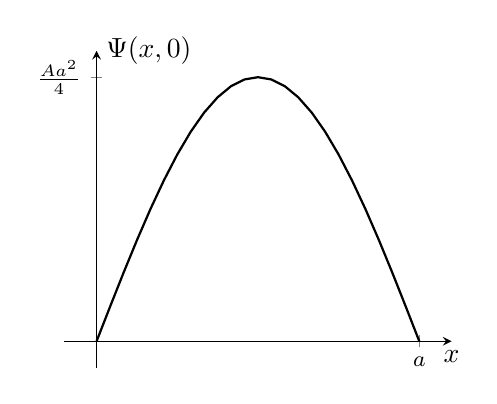
\begin{tikzpicture}
\begin{axis}[small,axis lines=middle,xlabel={$x$},ylabel={$\Psi(x,0)$},xtick={180},xticklabels={$a$},ytick={1},yticklabels={$\frac{Aa^2}{4}$},xlabel style={at={(current axis.right of origin)},anchor=north},ylabel style={at={(current axis.above origin)},anchor=west},enlargelimits]
\addplot[thick,domain=0:180]{sin(x)};
\end{axis}
\end{tikzpicture}
\caption{ابتدائی تفاعل موج برائے مثال \حوالہ{مثال_غیر_تابع_ابتدائی_تفاعل_موج}۔}
\label{شکل_غیر_تابع_ابتدائی_تفاعل_موج}
\end{figure}

حل:\quad
ہم پہلے \عددی{\Psi(x,0)} کو معمول پر لاتے ہوئے 
\begin{align*}
1=\int_{0}^{a}\abs{\Psi(x,0)}^{2}\dif{x}=\abs{A}^{2}\int_{0}^{a}x^{2}(a-x)^{2}\dif{x}=\abs{A}^{2}\frac{a^{5}}{30}
\end{align*}
\عددی{A} متعین کرتے ہیں۔ 
\begin{align*}
A=\sqrt{\frac{30}{a^{5}}}
\end{align*}
مساوات \حوالہ{مساوات_شروڈنگر_عددی_سروں} کے تحت \عددی{n} واں عددی سر درج ذیل ہو گا۔
\begin{align*}
c_{n}&=\sqrt{\frac{2}{a}}\int_{0}^{a}\sin\big(\frac{n\pi}{a}x\big)\sqrt{\frac{30}{a^{5}}}x(a-x)\dif{x}\\
&=\frac{2\sqrt{15}}{a^{3}}\Big[a\int_{0}^{a}x\sin\big(\frac{n\pi}{a}x\big)\dif{x}-\int_{0}^{a}x^{2}\sin\big(\frac{n\pi}{a}x\big)\dif x\Big]\\
&=\frac{2\sqrt{15}}{a^{3}}\Big\{a \left .\Big[\big(\frac{a}{n\pi}\big)^{2}\sin\big(\frac{n\pi}{a}x\big)-\frac{ax}{n\pi}\cos\big(\frac{n\pi}{a}x\big)\Big]\right\vert_{0}^{a}\.\\
&\quad-\left .\Big[2\big(\frac{a}{n\pi}\big)^{2}x\sin\big(\frac{n\pi}{a}x\big)-\frac{(n\pi x/a)^{2}-2}{(n\pi/a)^{3}}\cos\big(\frac{n\pi}{a}x\big)\Big]\right\vert_{0}^{a}\Big\}\\
&=\frac{2\sqrt{15}}{a^{3}}\Big[-\frac{a^{3}}{n\pi}\cos(n\pi)+a^{3}\frac{(n\pi)^{2}-2}{(n\pi)^{3}}\cos(n\pi)+a^{3}\frac{2}{(n\pi)^{3}}\cos(0)\Big]\\
&=\frac{4\sqrt{15}}{(n\pi)^{3}}[\cos(0)-\cos(n\pi)]\\
&=\begin{cases}
0 & \text{\RL{جفت $n$}}\\
8\sqrt{15}/(n\pi)^{3}& \text{\RL{طاق $n$}}
\end{cases}
\end{align*}
یوں تفاعل موج   درج ذیل ہو گا (مساوات \حوالہ{مساوات_شروڈنگر_ساکن_حالات_کا_مجموعہ})۔
 \begin{align*}
\Psi(x,t)=\sqrt{\frac{30}{a}}\big(\frac{2}{\pi}\big)^3\sum_{n=1,3,5\cdots}\frac{1}{n^3}\sin\big(\frac{n\pi}{a}x\big)e^{-in^{2}\pi^{2}\hslash t/2ma^{2}}
\end{align*}
\انتہا{مثال}
%
سر سری طور پر  ہم کہتے ہیں کہ \عددی{c_n}، " تفاعل \عددی{\Psi} میں \عددی{\psi_n} کی مقدار"  کو ظاہر کرتا ہے۔  بعض اوقات ہم کہتے ہیں کہ \عددی{n} ویں ساکن حال میں ایک ذرے کے  پائے جانے کا احتمال \عددی{\abs{c_n}^2} ہے جو درست نہیں،  چونکہ ذرہ حال \عددی{\Psi} میں ہے  نا کہ حال \عددی{\psi_n} میں؛ ویسے بھی،  تجربہ گاہ میں آپ کسی ایک ذرے  کو کسی ایک مخصوص حال میں نہیں دیکھ پاتے بلکہ آپ کسی \ترچھا{قابل مشاہدہ} مقدار  کی پیمائش کرتے ہیں، جس کا نتیجہ  ایک \ترچھا{عدد} کی صورت میں سامنے آتا ہے۔ جیسا کہ  آپ باب \حوالہ{باب_قواعد_و_ضوابط} میں دیکھیں گے، توانائی کی پیمائش سے \عددی{E_n} قیمت حاصل ہونے کا احتمال \عددی{\abs{c_n}^2} ہو گا۔ (کوئی بھی پیمائش، "اجازتی" قیمتوں میں سے کوئی ایک قیمت  دے گی، اسی لئے انہیں اجازتی قیمتیں کہتے ہیں، اور کوئی مخصوص قیمت \عددی{E_n} حاصل ہونے کا احتمال \عددی{\abs{c_n}^2} ہو گا۔)

یقیناً ان تمام احتمالات کا مجموعہ \عددی{1} ہونا چاہیے،
\begin{align}
\sum_{n=1}^{\infty}\abs{c_n}^2=1
\end{align}
جس کا ثبوت \عددی{\Psi} کی عمود زنی سے حاصل ہو گا (چونکہ تمام \عددی{c_n} غیر تابع وقت ہیں لہٰذا میں \عددی{t=0} پر اس کا  ثبوت پیش کرتا ہوں؛اگر آپ کو اس سے تشویش ہو تو  آپ باآسانی اس ثبوت کی تعمیم کسی بھی \عددی{t}  کے لئے کر سکتے ہیں۔)۔
\begin{align*}
1&=\int\abs{\Psi(x,0)}^2\dif x=\int \big(\sum_{m=1}^{\infty}c_m\psi_m(x)\big)^{\!*}\big(\sum_{n=1}^{\infty}c_n\psi_n(x)\big)\dif x\\
&=\sum_{m=1}^{\infty}\sum_{n=1}^{\infty}c_m^*c_n\int\psi_m(x)^*\psi_n(x)\dif x\\
&=\sum_{n=1}^{\infty}\sum_{m=1}^{\infty}c_m^*c_n\delta_{mn}=\sum_{n=1}^{\infty}\abs{c_n}^2
\end{align*}
(یہاں بھی \عددی{m} پر مجموعہ  میں کرونیکر ڈیلٹا جزو \عددی{m=n} کو چنتا ہے۔)

مزید یہ کہ  توانائی کی توقعاتی قیمت لازماً 
\begin{align}\label{مساوات_غیر_تابع_وقت_توانائی_توقعاتی_قیمت}
\langle H\rangle=\sum_{n=1}^{\infty} \abs{c_n}^2 E_n
\end{align} 
ہو گی   جس کی بلا واسطہ تصدیق کی جا سکتی ہے: غیر تابع وقت شروڈنگر مساوات (مساوات \حوالہ{مساوات_غیر_تابع_شروڈنگر_توانائی_مساوات}) کہتی ہے کہ
\begin{align}
H\psi_n=E_n\psi_n
\end{align}
لہٰذا
\begin{align*}
\langle H \rangle &=\int \Psi^*H\Psi\dif x=\int \big(\sum c_m\psi_m\big)^* H\big(\sum c_n\psi_n\big)\dif x\\
&=\sum\sum c_m^*c_nE_n\int \psi_m^*\psi_n\dif x=\sum\abs{c_n}^2 E_n
\end{align*}
ہو گا۔ دھیان رہے کہ کسی ایک مخصوص توانائی کے حصول کا احتمال غیر تابع وقت ہو گا اور یوں \عددی{H} کی توقعاتی قیمت حتماً  غیر تابع وقت ہو گی۔ کوانٹم میکانیات میں یہ \اصطلاح{بقا توانائی}\فرہنگ{بقا!توانائی}\حاشیہب{conservation of energy}\فرہنگ{energy!conservation} کا ظہور ہے۔

\ابتدا{مثال}\شناخت{مثال_شروڈنگر_عددی_سر_توقعاتی}
ہم نے دیکھا کہ مثال \حوالہ{مثال_غیر_تابع_ابتدائی_تفاعل_موج} میں ابتدائی تفاعل موج (شکل \حوالہ{شکل_غیر_تابع_ابتدائی_تفاعل_موج}) زمینی حال \عددی{\psi_{1}} (شکل \حوالہ{شکل_غیر_تابع_لامتناہی_چکور_تین_ساکن_حالات}) کے ساتھ قریبی مشابہت رکھتا ہے۔ یوں ہم توقع کریں گے کہ \عددی{|c_1|^2} غالب ہو گا۔ یقیناً ایسا ہی ہے۔
\begin{align*}
\left| c_{1} \right|^{2} = \left( \frac{8\sqrt{15}}{\pi^{3}} \right)^{2} = 0.998555 \dotso
\end{align*}
باقی تمام عددی سر مل کر درج ذیل فرق دیتے ہیں۔\حاشیہد{آپ درج ذیل تسلسل کسی ریاضی کی کتاب سے دیکھ سکتے ہیں۔
\begin{align*}
\frac{1}{1^6}+\frac{1}{3^6}+\frac{1}{5^6}+\cdots&=\frac{\pi^6}{960}\\
\frac{1}{1^4}+\frac{1}{3^4}+\frac{1}{5^4}+\cdots&=\frac{\pi^4}{96}
\end{align*}
}
\begin{align*}
\sum_{n=1}^{\infty} \left| c_{n} \right|^{2} = \left( \frac{8\sqrt{15}}{\pi^{3}} \right)^{2} \sum_{n=1,3,5,...}^{\infty} \frac{1}{n^{6}} = 1
\end{align*}
اس مثال میں توانائی کی توقعاتی قیمت
\begin{align*}
\langle H \rangle = \sum_{n=1,3,5,...}^{\infty} \left( \frac{8\sqrt{15}}{n^{3} \pi^{3}} \right)^{2} \frac{n^{2} \pi^{2} \hslash^{2}}{2ma^{2}} = \frac{480\hslash^{2}}{\pi^{4} ma^{2}} \sum_{n=1,3,5,...}^{\infty} \frac{1}{n^{4}} = \frac{5 \hslash^{2}}{ma^{2}}
\end{align*}
 ہو گی جو کہ ہماری توقعات کے عین مطابق  ہے۔  یہ \عددی{ E_{1} = \pi^{2} \hslash^{2}/2ma^{2} } کے بہت قریب ، مگر ہیجان حالتوں  کی شمولیت کی بنا پر  تھوڑی زیادہ ہے۔ 
\انتہا{مثال}
%===========
\ابتدا{سوال}\شناخت{سوال_شروڈنگر_حل_ناقابل_قبول}
یہ دکھائیں کہ لا متناہی چوکور کنویں  کے لئے \عددی{ E = 0 } یا \عددی{ E < 0 } کی صورت میں غیر تابع وقت شروڈنگر مساوات کا کوئی بھی قابل قبول حل نہیں پایا جاتا۔ (یہ سوال \حوالہ{سوال_شروڈنگر_کم_سے_کم_توانائی} میں دیے گئے عمومی مسئلے کی ایک مخصوص صورت ہے، لیکن اس  مرتبہ  شروڈنگر مساوات کو صریحاً حل کرتے ہوئے دکھائیں کہ آپ سرحدی شرائط   کو پورا نہیں کر  سکتے۔)
 \انتہا{سوال}
%==============
\ابتدا{سوال}\شناخت{سوال_غیر_تابع_لامتناہی_این_ویں}
لامتناہی چوکور کنویں  کے \عددی{ n } وی ساکن حال کیلئے \عددی{\langle x \rangle}، \عددی{\langle x^2 \rangle} ، \عددی{\langle p \rangle}، \عددی{\langle p^2 \rangle}، \عددی{\sigma_x}،  اور \عددی{\sigma_p} تلاش کریں۔ تصدیق کریں کہ اصول غیر یقینیت مطمئن ہوتا ہے۔ کونسا حال غیر یقینیت کی حد کے قریب ترین ہو گا؟
\انتہا{سوال}
%=============
\ابتدا{سوال}\شناخت{سوال_شروڈنگر_لامتناہی_کنواں_برابر_حصے}
لامتناہی چوکور کنویں  میں ایک ذرے کا ابتدائی تفاعل موج،   پہلے  دو ساکن  حالات  کے برابر  حصوں کا مرکب ہے۔ 
\begin{align*}
\Psi(x,0) = A[\psi_{1}(x) + \psi_{2}(x)]
\end{align*}
\begin{enumerate}[a.]
\item 
\عددی{ \Psi(x,0) } کو معمول پر لائیں۔ (یعنی \عددی{ A } تلاش کریں۔ آپ \عددی{ \psi_{1} } اور \عددی{ \psi_{2} } کی معیاری عمودیت  کا فائدہ اٹھاتے  ہوئے با آسانی ایسا کر سکتے ہیں۔ یاد رہے کہ \عددی{ t=0 } پر \عددی{ \Psi } کو معمول پر لانے کے بعد آپ یقین رکھ سکتے ہیں کہ یہ معمول شدہ ہی رہے گا؛  اگر آپ کو شک ہو تو  جزو-ب کا نتیجہ حاصل کرنے کے بعد اس کی صریحاً تصدیق کریں۔) 
\item
\عددی{ \Psi(x,t) } اور \عددی{ \left| \Psi (x,t) \right|^{2} } تلاش کریں۔ موخر الذکر کو وقت کے سائن نما تفاعل کی صورت میں لکھیں، جیسا مثال \حوالہ{مثال_غیر_تابع_دو_ساکن_حالات_ذرہ} میں کیا گیا ہے۔ نتائج کی  تسہیل  کے لئے  \عددی{\omega\equiv\tfrac{\pi^2\hslash}{2ma^2}} لیں۔ 
\item 
\عددی{ \langle x \rangle } تلاش کریں۔ آپ دیکھیں گے کہ یہ وقت میں  ارتعاش  پذیر  ہے۔ اس ارتعاش کا  زاویائی تعدد کتنا ہو گا؟ ارتعاش کا حیطہ کیا ہو گا؟ (اگر  حیطہ \عددی{ \tfrac{a}{2}} سے زیادہ نکل آئے تو  آپ  سیدھا    قید خانے  چلے جائیں۔) 
\item 
\عددی{ \langle p \rangle } تلاش کریں (اور اس پر  زیادہ وقت صرف نہ کریں)۔ 
\item
اس ذرے کی توانائی کی پیمائش کی جائے  تو  کون کون سی قیمتیں متوقع ہوں گی اور ہر ایک قیمت کا احتمال کتنا ہو گا؟ \عددی{ H } کی توقعاتی قیمت تلاش کریں۔ اس کی قیمت کا موازنہ \عددی{ E_{1} } اور \عددی{ E_{2} } کے ساتھ کریں؟
\end{enumerate}
\انتہا{سوال}
%================
\ابتدا{سوال}
اگرچہ تفاعل موج کا \ترچھا{ مجموعی}  زاویائی مستقل کسی  طبیعی اہمیت کا حامل نہیں ہے (کیونکہ یہ کسی بھی قابل پیمائش مقدار کا حساب کرتے ہوئے منسوخ ہو جاتا ہے) لیکن مساوات \حوالہ{مساوات_شروڈنگر_عمومی_حل_مجموعہ} میں عددی سروں کے اضافی زاویائی مستقل اہمیت کے حامل ہیں۔ مثال کے طور پر، فرض کریں کہ  ہم سوال \حوالہ{سوال_شروڈنگر_لامتناہی_کنواں_برابر_حصے} میں \عددی{ \psi_{1} } اور \عددی{ \psi_{2} } کے اضافی زاویائی مستقل تبدیل کر دیتے  ہیں:
\begin{align*}
\Psi (x,0) = A[\psi_{1} (x) + e^{i\phi}\psi_{2}(x)]
\end{align*}
یہاں \عددی{ \phi } کوئی مستقل ہے۔ \عددی{ \Psi(x,t) }، \عددی{ \ \left| \Psi (x,t) \right|^{2} } اور \عددی{ \langle x \rangle } تلاش کر کے ان کا موازنہ پہلے حاصل شدہ نتائج کے ساتھ کریں۔ بالخصوص \عددی{ \phi = \pi/2 } اور \عددی{ \phi = \pi } کی صورتوں پر غور کریں۔ 
\انتہا{سوال}
%===========
\ابتدا{سوال} \شناخت{سوال_غیر_تابع_شروڈنگر_ابتدائی_تفاعل_موج_چکور_کنواں}
لا متناہی چوکور کنویں  میں ایک ذرے کا ابتدائی تفاعل موج درج ذیل ہے۔\حاشیہد{اصولی طور پر ابتدائی تفاعل موج کی شکل   پر کوئی پابندی عائد نہیں ہوتی،  جب تک کہ وہ  معمول پر لانے کے قابل  رہے۔ بالخصوص، ضروری نہیں کہ \عددی{\Psi(x,0)} کا استمراری تفرق پایا جاتا ہو؛  بلکہ تفاعل کا خود استمراری ہونا بھی ضروری نہیں ہے۔تاہم، اگر آپ   \عددی{\langle H\rangle} کی قیمت  کو   \عددی{\int\Psi(x,0)^*H\Psi(x,0)\dif x} سے  معلوم کرنا چاہیں  گے تو آپ کو تکنیکی مشکلات کا سامنا کرنا پڑے گا، اس لئے کہ    \عددی{\Psi(x,0)}  کا دوم تفرق بد معین ہے۔ سوال \حوالہ{سوال_غیر_تابع_دوسرا_تفرق_عدم_واضح} میں ایسا کرنا اس لئے ممکن ہوا کہ  عدم استمرار آخری سروں پر پائے گئے جہاں تفاعل خود صفر ہے۔ سوال \حوالہ{سوال_غیر_تابع_شروڈنگر_ابتدائی_تفاعل_موج_چکور_کنواں} کی طرح کے مسائل کو حل کرنا آپ سوال \حوالہ{سوال_غیر_تابع_ترکیب_کی_وضاحت} میں دیکھیں گے۔}
\begin{align*}
\Psi (x,0) = 
\begin{cases}
Ax, & 0 \leq x \leq a/2 \\ 
A(a-x), & a/2 \leq x \leq a
\end{cases}
\end{align*}
\begin{enumerate}[a.]
\item 
\عددی{\Psi(x,0)} کا خاکہ کھینچیں اور مستقل \عددی{A} کی قیمت تعین  کریں۔
\item 
\عددی{\Psi(x,t) } تلاش کریں۔
\item 
توانائی کی پیمائش کا نتیجہ \عددی{E_{1}} ہونے کا احتمال کتنا ہو گا؟
\item 
توانائی کی توقعاتی قیمت تلاش کریں۔
\end{enumerate}
\انتہا{سوال}
%===========
\ابتدا{سوال}
ایک ذرہ جس کی کمیت \عددی{m} ہے ابتدا   \عددی{(t=0)}  میں  لامتناہی چوکور کنویں   (چوڑائی \عددی{a})  کے نصف بائیں  حصے میں  پایا جاتا ہے جہاں ہر نقطے پر اس کے ہونے کا  امکان  ایک جیسا  ہے۔ 
\begin{enumerate}[a.]
\item
اس کا  ابتدائی تفاعل موج \عددی{\Psi(x,0) } تلاش کریں۔ (فرض کریں کے یہ حقیقی ہے۔  اسے معمول پر لانا  مت بھولیں۔)
\item 
توانائی کی پیمائش  کے  نتیجے  میں  \عددی{\pi^{2}\hslash^{2}/2ma^{2}} ملنے  کا احتمال کیا ہو گا؟ 
\end{enumerate} 
\انتہا{سوال}
%==========
\ابتدا{سوال}\شناخت{سوال_غیر_تابع_دوسرا_تفرق_عدم_واضح}
لمحہ \عددی{t=0} پر مثال \حوالہ{مثال_غیر_تابع_ابتدائی_تفاعل_موج} کے تفاعل موج کیلئے \عددی{H} کی توقعاتی قیمت  "پرانے دقیانوسی طریقہ":
\begin{align*}
\langle H \rangle=\int \Psi(x,0)^*\hat{H}\, \Psi(x,0)\dif x
\end{align*}
سے   حاصل کریں۔  مثال \حوالہ{مثال_شروڈنگر_عددی_سر_توقعاتی} میں مساوات \حوالہ{مساوات_غیر_تابع_وقت_توانائی_توقعاتی_قیمت} کی مدد سے حاصل کردہ نتیجے کے ساتھ اس کا  موازنہ کریں۔  \ترچھا{توجہ کریں:}  کیونکہ \عددی{H} غیر تابع وقت ہے لہٰذا \عددی{t=0} لینے سے نتیجے پر کوئی اثر نہیں ہو گا۔ 
\انتہا{سوال}
%=========================
%%% KKKK edited till here with dr fakhar inam 23 dec 20201
 \حصہ{ہارمونی مرتعش}
کلاسیکی ہارمونی مرتعش ایک لچک دار اسپرنگ جس کا مقیاس لچک \عددی{k} ہو اور کمیت \عددی{m} پر مشتمل ہوتا ہے۔ کمیت کی حرکت \اصطلاح{قانون ہک}\فرہنگ{قانون!ہک}\حاشیہب{Hooke's law}\فرہنگ{law!Hooke} 
\begin{align*}
F=-kx=m\frac{\dif{^{2}x}}{\dif{t^{2}}}
\end{align*}
کے تحت ہو گی جہاں رگڑ کو نظر انداز کیا گیا ہے۔ اس کا حل
\begin{align*}
x(t)=A\sin(\omega t)+B\cos(\omega t)
\end{align*}
ہو گا جہاں
\begin{align}\label{مساوات_شروڈنگر_زاویائی_تعدد}
\omega\equiv \sqrt{\frac{k}{m}}
\end{align}
ارتعاش کا (زاویائی) تعدد ہے۔ مخفی توانائی
\begin{align}
V(x)=\frac{1}{2}kx^{2}
\end{align}
ہو گی جس کی ترسیم قطع مکافی ہے۔ 

\begin{figure}
\centering
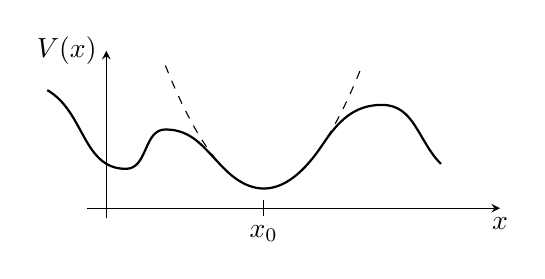
\begin{tikzpicture}
\pgfmathsetmacro{\kx}{1.5}
\pgfmathsetmacro{\ky}{(\kx-2)^2+0.25}
\pgfmathsetmacro{\m}{2*(\kx-2)}
\pgfmathsetmacro{\ang}{180+atan(\m)}
\pgfmathsetmacro{\kkx}{2.75}
\pgfmathsetmacro{\kky}{(\kkx-2)^2+0.25}
\pgfmathsetmacro{\km}{2*(\kkx-2)}
\pgfmathsetmacro{\kang}{atan(\km)}
\draw[-stealth](-0.25,0)--(5,0)node[below]{$x$};
\draw[-stealth](0,-0.125)--(0,2)node[left]{$V(x)$};
\draw [dashed,domain=0.75:3.25,smooth,variable=\x] plot ({\x},{(\x-2)^2+0.25}); 
\draw [thick,domain=1.5:2.75,smooth,variable=\x] plot ({\x},{(\x-2)^2+0.25}); 
\draw[thick](\kx,\ky) to [out=\ang,in=0]++(-0.75,0.5) to [out=180,in=0] ++(-0.5,-0.5) to [out=180,in=-30]++(-1,1);
\draw[thick](\kkx,\kky) to [out=\kang,in=180]++(0.75,0.5) to [out=0,in=135]++(0.75,-0.75);
\draw(2,0)++(0,0.1)--++(0,-0.2)node[below]{$x_0$};
\end{tikzpicture} 
\caption{اختیاری مخفیہ کے مقامی کم سے کم قیمت نقطہ کی پڑوس میں قطع مکافی تخمین (نقطہ دار ترسیم)۔}
\label{شکل_غیر_تابع_مقامی_کم_سے_کم_قطع_مکافی}
\end{figure}

حقیقت میں کامل ہارمونی مرتعش نہیں پایا جاتا ہے۔ اگر آپ اسپرنگ کو زیادہ کھینچیں تو وہ ٹوٹ جائے گا اور قانون ہک اس سے بہت پہلے غیر کارآمد ہو چکا ہو گا۔ تاہم عملاً کوئی بھی مخفیہ، مقامی کم سے کم نقطہ کی پڑوس میں تخمیناً قطع مکافی
 ہو گا (شکل \حوالہ{شکل_غیر_تابع_مقامی_کم_سے_کم_قطع_مکافی})۔مخفی توانائی \عددی{V(x)} کے کم سے کم نقطہ \عددی{x_0} کے لحاظ سے \عددی{V(x)} کو \اصطلاح{ٹیلر تسلسل}\فرہنگ{تسلسل!ٹیلر}\حاشیہب{Taylor series}\فرہنگ{series!Taylor} کے لحاظ سے پھیلا کر
\begin{align*}
V(x)=V( x_{0})+V'(x_{0})(x-x_{0})+\frac{1}{2}V''(x_{0})(x-x_{0})^{2}+\cdots
\end{align*}
اس سے \عددی{V(x_0)} منفی کر کے (ہم \عددی{V(x)} سے کوئی بھی مستقل بغیر خطر و فکر منفی کر سکتے ہیں کیونکہ ایسا کرنے سے قوت تبدیل نہیں ہو گا) اور یہ جانتے ہوئے کہ \عددی{V'(x_0)=0} ہو گا (چونکہ \عددی{x_0} کم سے کم نقطہ ہے)، ہم تسلسل کے بلند رتبی ارکان رد کرتے ہوئے (جو \عددی{(x-x_0)} کی قیمت کم ہونے کی صورت میں قابل نظرانداز ہونگے) درج ذیل حاصل کرتے ہیں
\begin{align*}
V(x)\cong\frac{1}{2}V''(x_{0})(x-x_{0})^{2}
\end{align*}
جو نقطہ \عددی{x_0} پر ایک ایسی سادہ ہارمونی ارتعاش بیان کرتا ہے جس کا موثر مقیاس لچک \عددی{k=V''(x_0)} ہو۔\حاشیہد{چونکہ ہم فرض کر رہے ہیں کہ \عددی{x_0} کم سے کم نقطہ ہے لہٰذا \عددی{V''(x_0)\ge 0} ہو گا۔صرف اس نایاب صورت میں ارتعاش تخمینی طور پر بھی سادہ ہارمونی نہیں ہو گا   جب \عددی{V''(x_0)=0} ہو۔} یہی وہ وجہ ہے جس کی بنا پر سادہ ہارمونی مرتعش اتنا اہم ہے: تقریباً ہر وہ ارتعاشی حرکت جس کا حیطہ کم ہو تخمیناً سادہ ہارمونی ہو گا۔

کوانٹم میکانیات میں ہمیں مخفیہ
\begin{align}\label{مساوات_شروڈنگر_مخفیہ_ہارمونی}
V(x)=\frac{1}{2}m\omega ^{2}x^{2}
\end{align}
کے لیے شروڈنگر مساوات حل کرنی ہو گی (جہاں روایتی طور پر مقیاس لچک کی جگہ کلاسیکی تعدد (مساوات \حوالہ{مساوات_شروڈنگر_زاویائی_تعدد}) استعمال کی جاتی ہے)۔ جیسا کہ ہم دیکھ چکے ہیں، اتنا کافی ہو گا کہ ہم غیر تابع وقت شروڈنگر مساوات
\begin{align}\label{مساوات_شروڈنگر_مخفی_قوہ_الف}
\frac{-\hslash ^{2}}{2m}\frac{\dif{^{2}\psi}}{\dif{x^{2}}}+\frac{1}{2}m\omega ^{2}x^{2}\psi=E\psi
\end{align}
حل کریں۔ اس مسئلے کو حل کرنے کے لیے دو بالکل مختلف طریقے اپنائے جاتے ہیں۔ پہلی میں تفرقی مساوات کو "طاقت کے بل بوتے پر" \اصطلاح{طاقتی تسلسل}\فرہنگ{تسلسل!طاقتی}\حاشیہب{power series}\فرہنگ{series!power} کے ذریعہ حل کرنے کی ترکیب استعمال کی جاتی ہے، جو دیگر مخفیہ کے لیے بھی کارآمد ثابت ہوتا ہے (اور جسے استعمال کرتے ہوئے ہم باب \حوالہ{باب_تین_ابعادی_کوانٹم_میکانیات} میں کولمب مخفیہ کے لیے حل تلاش کریں گے)۔ دوسری ترکیب ایک شیطانی الجبرائی تکنیک ہے جس میں \اصطلاح{عاملین سیڑھی} استعمال ہوتے ہیں۔ میں آپ کی واقفیت پہلے الجبرائی تکنیک کے ساتھ پیدا کرتا ہوں جو زیادہ سادہ، زیادہ دلچسپ (اور حل جلد ی دیتا)\حاشیہد{یہی تراکیب زاویائی معیار حرکت کے نظریہ (باب \حوالہ{باب_تین_ابعادی_کوانٹم_میکانیات}) میں مستعمل ہیں اور انہیں عمومیت دیتے ہوئے \اصطلاح{عمدہ تشاکلی کوانٹم میکانیات} کے  مخفیہ کی وسیع جماعت کے لئے استعمال کیا جا سکتا ہے۔} ہے۔ اگر آپ طاقتی تسلسل کی ترکیب یہاں استعمال نہ کرنا چاہیں تو آپ ایسا کر سکتے ہیں لیکن کہیں نہ کہیں آپکو یہ ترکیب سیکھنی ہو گی۔

\جزوحصہ{الجبرائی ترکیب}\شناخت{حصہ_غیر_تابع_وقت_شروڈنگر_الجبرائی_ترکیب}
ہم مساوات \حوالہ{مساوات_شروڈنگر_مخفی_قوہ_الف} کو زیادہ معنی خیز روپ میں لکھ کر ابتدا کرتے ہیں
\begin{align}
\frac{1}{2m}[p^{2}+(m\omega x)^{2}]\psi=E\psi
\end{align}
جہاں \عددی{p\equiv \frac{\hslash}{i}\frac{d}{\dif{x}}} معیار حرکت کا عامل ہے۔ بنیادی طور پر ہیملٹنی
\begin{align}
H=\frac{1}{2m}[p^{2}+(m\omega x)^{2}]
\end{align}
کو کو \ترچھا{اجزائے ضربی} لکھنے کی ضرورت ہے۔اگر یہ عداد ہوتے تب ہم یوں لکھ سکتے تھے۔
\begin{align*}
u^{2}+v^{2}=(iu+v)(-iu+v)
\end{align*}
البتہ یہاں بات اتنی سادہ نہیں ہے چونکہ \عددی{p} اور \عددی{x} \ترچھا{عاملین} ہیں اور عاملین عموماً \اصطلاح{مقلوب}\فرہنگ{مقلوب}\حاشیہب{commute}\فرہنگ{commute} نہیں ہوتے ہیں (یعنی آپ \عددی{xp} سے مراد \عددی{px} نہیں لے سکتے ہیں)۔ اس کے باوجود یہ ہمیں درج ذیل مقداروں پر غور کرنے پر آمادہ کرتا ہے
\begin{align}\label{مساوات_شروڈنگر_تعریفات_سیڑھی}
a\pm\equiv \frac{1}{\sqrt{2\hslash m\omega}}(\mp ip+m\omega x)
\end{align}
(جہاں قوسین کے باہر جزو ضربی لگانے سے آخری نتیجہ خوبصورت نظر آئے گا)۔

آئیں دیکھیں حاصل ضرب \عددی{a_{-}a_{+}} کیا ہو گا؟
\begin{align*}
a_{-}a_{+}&=\frac{1}{2\hslash m\omega}(ip+m\omega x)(-ip+m\omega x)\\
&=\frac{1}{2\hslash m\omega}[p^{2}+(m\omega x)^{2}-im\omega(xp-px)]
\end{align*}
اس میں متوقع اضافی جزو \عددی{(xp-px)} پایا جاتا ہے جس کو ہم \عددی{x} اور \عددی{p} کا \اصطلاح{مقلب}\فرہنگ{مقلب}\حاشیہب{commutator}\فرہنگ{commutator} کہتے ہیں اور جو ان کی آپس میں مقلوب   نہ ہونے کی پیمائش ہے۔ عمومی طور پر عامل \عددی{A} اور عامل \عددی{B} کا مقلب (جسے چوکور قوسین میں لکھا ہے) درج ذیل ہو گا۔
\begin{align}\label{مساوات_غیر_تابع_شروڈنگر_تبادل_کار}
[A,B]\equiv AB-BA
\end{align}
اس علامتیت کے تحت درج ذیل ہو گا۔
\begin{align}\label{مساوات_شروڈنگر_سیڑھی_حاصل_ضرب}
a_{-}a_{+}=\frac{1}{2\hslash m\omega}[p^{2}+(m\omega x)^{2}]-\frac{i}{2\hslash}[x,p]
\end{align}

ہمیں \عددی{x} اور عددی{p} کا مقلب دریافت کرنا ہو گا۔ \ترچھا{انتباہ:} عاملین پر ذہنی کام کرنا عموماً غلطی کا سبب بنتا ہے۔ بہتر ہو گا کہ عاملین پرکھنے کے لیے آپ انہیں تفاعل \عددی{f(x)} عمل کرنے کے لئے پیش کریں۔ آخر میں اس پرکھی تفاعل کو رد کر کے آپ صرف عاملین پر مبنی مساوات حاصل کر سکتے ہیں۔ موجودہ صورت میں درج ذیل ہو گا۔
\begin{align}
[x,p]f(x)=\big[x\frac{\hslash}{i}\frac{\dif}{\dif{x}}(f)-\frac{\hslash}{i}\frac{\dif}{\dif{x}}(xf)\big ]=\frac{\hslash}{i}\big (x\frac{\dif{f}}{\dif{x}}-x\frac{\dif{f}}{\dif{x}}-f\big )=-i\hslash f(x)
\end{align}
پرکھی تفاعل (جو اپنا کام کر چکا) کو رد کرتے ہوئے درج ذیل ہو گا۔
\begin{align}\label{مساوات_غیر_تابع_شروڈنگر_مقام_معیار_حرکت_تبادل_کار}
[x,p]=i\hslash
\end{align}
یہ خوبصورت نتیجہ جو بار بار سامنے آتا ہے \اصطلاح{باضابطہ مقلبیت رشتہ}\فرہنگ{مقلبیت!باضابطہ رشتہ}\حاشیہب{canonical commutation relation}\فرہنگ{commutation!canonical relation} کہلاتا\حاشیہد{گہری نظر سے دیکھا جائے تو کوانٹم میکانیات کے تمام طلسمات کا دارومدار اس حقیقت پر ہے کہ مقام اور معیار حرکت آپس میں مقلوب نہیں ہیں۔ بعض مصنفین باضابطہ مقلبیت رشتہ کو مسلمہ لیتے ہوئے \عددی{p=(\hslash/i)\dif/\dif x} اخذ کرتے ہیں۔} ہے۔

اسے کے استعمال سے مساوات \حوالہ{مساوات_شروڈنگر_سیڑھی_حاصل_ضرب} درج ذیل روپ 
\begin{align}
a_{-}a_{+}=\frac{1}{\hslash\omega}H+\frac{1}{2}
\end{align}
یا
\begin{align}
H=\hslash\omega\big (a_{-}a_{+}-\frac{1}{2} \big )
\end{align}
اختیار کرتی ہے۔ آپ نے دیکھا کہ ہیملٹنی کو ٹھیک اجزائے ضربی کی صورت میں نہیں لکھا جا سکتا اور دائیں ہاتھ اضافی \عددی{-\tfrac{1}{2}} ہو گا۔ یاد رہے گا یہاں \عددی{a_+} اور \عددی{a_-} کی ترتیب بہت اہم ہے۔ اگر آپ \عددی{a_+} کو بائیں طرف رکھیں تو درج ذیل حاصل ہو گا۔
\begin{align}
a_{+}a_{-}=\frac{1}{\hslash\omega}H-\frac{1}{2}
\end{align}
بالخصوص درج ذیل ہو گا۔
\begin{align}\label{مساوات_شروڈنگر_سیڑھی_ضرب_برابر_اکائی}
[a_{-},a_{+}]=1
\end{align}
یوں ہیملٹنی کو درج ذیل بھی لکھا جا سکتا ہے۔
\begin{align}
H=\hslash\omega\big (a_{+}a_{-}+\frac{1}{2}\big )
\end{align}


ہارمونی مرتعش کی شروڈنگر مساوات\حاشیہد{میں بار بار "غیر تابع وقت شروڈنگر مساوات" کہہ کر تھک گیا ہوں لہٰذا جہاں متن سے واضح ہو کہ میں کس قسم کی مساوات کی بات کر رہا ہوں، میں اس کو "شروڈنگر مساوات" پکاروں گا۔} کو \عددی{a_{\pm}} کی صورت میں درج ذیل لکھا جا سکتا ہے۔
\begin{align}\label{مساوات_شروڈنگر_عوامل_روپ}
 \hslash \omega \big(a_{\pm} a_{\mp} \,\pm \frac{1}{2}\big)=E\psi 		
\end{align}
(اس طرح کی مساوات میں آپ یا تو بالائی علامتیں ایک ساتھ پڑھتے ہو اور یا زیریں علامتیں ایک ساتھ پڑھتے ہو۔)

 ہم ایک اہم موڑ پر ہیں۔ میں دعویٰ کرتا ہوں اگر توانائی \عددی{E} کی شروڈنگر مساوات کو \عددی{ \psi } مطمئن کرتا ہو 
 \عددی{ ( H \psi = E \psi ) } تب توانائی \عددی{(E+\hslash \omega)} کی شروڈنگر مساوات کو \عددی{a_+ \psi } مطمئن کرے گا: \عددی{ H ( a_+ \psi ) = ( E + \hslash \omega) ( a_+ \psi ) }

ثبوت:
\begin{align*}
H ( a_+ \psi ) &= \hslash \omega ( a_+ a_- + \frac{1}{2}) (a_+ \psi) = \hslash \omega (a_+ a_- a_+ + \frac{1}{2} a_+) \psi
\\
 &= \hslash \omega a_+ ( a_- a_+ + \tfrac{1}{2} ) \psi = a_+\big[ \hslash \omega ( a_+ a_- + 1 + \tfrac{1}{2} ) \psi \big ]\\
 &= a_+ ( H + \hslash \omega ) \psi = a_+ ( E + \hslash \omega ) \psi = ( E + \hslash \omega ) ( a_+ \psi )
\end{align*} 
(میں نے دوسری لکیر میں مساوات \حوالہ{مساوات_شروڈنگر_سیڑھی_ضرب_برابر_اکائی} استعمال کرتے ہوئے \عددی{ a_- a_+ }
 کی جگہ \عددی{ a_+ a_- + 1} استعمال کیا ہے۔ دھیان رہے اگرچہ \عددی{ a_+} اور \عددی{ a_- } کی ترتیب اہمیت کا حامل ہے، 
\عددی{ a \pm } اور کسی بھی مستقل، مثلاً \عددی{ \hslash }، \عددی{ \omega} اور E، کی ترتیب اہم نہیں ہے۔ ایک عامل ہر مستقل کے ساتھ مقلوب ہو گا۔)

 اسی طرح حل \عددی{ a_- \psi } کی توانائی \عددی{ ( E - \hslash \omega) } ہو گی۔
\begin{align*}
H(a_- \psi ) &= \hslash \omega ( a_- a_+ - \tfrac{1}{2}) (a_- \psi) = \hslash \omega a_- \,( a_+ a_- - \tfrac{1}{2} ) \psi\\
&= a_- \big[ \hslash \omega ( a_- a_+ - 1 - \tfrac{1}{2} ) \psi \big] = a_- ( H - \hslash \omega )\psi = a_- ( E - \hslash \omega) \psi \\	
&=( E - \hslash \omega ) ( a_- \psi )
\end{align*}
یوں ہم نے ایک ایسی خودکار ترکیب دریافت کر لی ہے جس سے، کسی ایک حل کو جانتے ہوئے، بالائی اور زیریں توانائی کے نئے حل دریافت کیے جا سکتے ہیں۔ چونکہ \عددی{ a \pm } کے ذریعے ہم توانائی میں اوپر چڑھ یا نیچے اتر سکتے ہیں لہٰذا انہیں ہم \اصطلاح{عاملین سیڑھی}\فرہنگ{سیڑھی!عاملین}\حاشیہب{ladder operators}\فرہنگ{ladder!operators} پکارتے ہیں: \عددی{ a_+ } \اصطلاح{عامل رفعت}\فرہنگ{عامل!رفعت}\حاشیہب{raising operator}\فرہنگ{operator!raising} اور \عددی{ a_- } \اصطلاح{عامل تقلیل}\فرہنگ{عامل!تقلیل}\حاشیہب{lowering operator}\فرہنگ{operator!lowering} ہے۔ عامل رفعت کو رفعتی عامل اور عامل تقلیل کو تقلیلی عامل بھی پکارا جاتا ہے۔حالات کی "سیڑھی" کو شکل \حوالہ{شکل_غیر_تابع_بلی_چڑھ_رہی_ہے} میں دکھایا گیا ہے۔

\begin{figure}
\centering
\begin{tikzpicture}[font=\small]
\pgfmathsetmacro{\ang}{60}
\pgfmathsetmacro{\kt}{0.1}
\pgfmathsetmacro{\kx}{1}
\pgfmathsetmacro{\kL}{8}
\pgfmathsetmacro{\kdL}{\kL/10}
\pgfmathsetmacro{\kddL}{0.1}
\draw(0,0)--++(\ang:\kL)--++(-\kt,0)--++(\ang:-\kL)--++(\kt,0);
\draw(\kx,0)--++(\ang:\kL)--++(\kt,0)--++(\ang:-\kL)--++(-\kt,0);
\foreach \n in {1,2,...,9}{
\draw(\ang:\n*\kdL)--++(\kx,0)++(\ang:\kddL)--++(-\kx,0);}
\draw(\ang:1*\kdL+\kddL)++(-0.1,0) node[left]{$E_0$}++(\kx+0.1+0.1,0)node[right]{$\psi_0$};
\draw(\ang:4*\kdL+\kddL)++(-0.1,0) node[left]{$E-2\hslash\omega$}++(\kx+0.1+0.1,0)node[right]{$a_-^2\psi$};
\draw(\ang:5*\kdL+\kddL)++(-0.1,0) node[left]{$E-\hslash\omega$}++(\kx+0.1+0.1,0)node[right]{$a_-\psi$};
\draw(\ang:6*\kdL+\kddL)++(-0.1,0) node[left]{$E$}++(\kx+0.1+0.1,0)node[right]{$\psi$};
\draw(\ang:7*\kdL+\kddL)++(-0.1,0) node[left]{$E+\hslash\omega$}++(\kx+0.1+0.1,0)node[right]{$a_+\psi$};
\draw(\ang:8*\kdL+\kddL)++(-0.1,0) node[left]{$E+2\hslash\omega$}++(\kx+0.1+0.1,0)node[right]{$a_+^2\psi$};
\draw(\ang:9*\kdL+\kddL)++(-0.1,0) node[left]{$E+3\hslash\omega$}++(\kx+0.1+0.1,0)node[right]{$a_+^3\psi$};
\draw[-latex,thick](\ang:10*\kdL)++(0.5*\kx,0)--++(\ang:0.5)node[above]{$E$};
\draw[-latex,thick]($(\ang:2*\kdL)+(\kx+1.5,0)$)--++(\ang:-1)node[right]{$a_-$};
\draw[-latex,thick]($(\ang:7*\kdL)+(\kx+1.5,0)$)--++(\ang:1)node[right]{$a_+$};
\end{tikzpicture}
\caption{ہارمونی مرتعش کے حالات کی "سیڑھی"۔}
\label{شکل_غیر_تابع_بلی_چڑھ_رہی_ہے}
\end{figure}
ذرا رکیے! عامل تقلیل کے بار بار استعمال سے آخرکار ایسا حل حاصل ہو گا جس کی توانائی صفر سے کم ہو گی ( جو سوال \حوالہ{سوال_شروڈنگر_کم_سے_کم_توانائی} میں پیش عمومی مسئلہ کے تحت نا ممکن ہے۔) نئے حالات حاصل کرنے کی خودکار ترکیب کسی نہ کسی نقطہ پر لازماً ناکامی کا شکار ہو گی۔ ایسا کیوں کر ہو گا؟ ہم جانتے ہیں کہ \عددی{ a_- \psi } شروڈنگر مساوات کا ایک نیا حل ہو گا، تاہم اس کی ضمانت نہیں دی جا سکتی ہے کہ یہ معمول پر لانے کے قابل بھی ہو گا؛ یہ صفر ہو سکتا ہے یا اس کا مربع تکمل لامتناہی ہو سکتا ہے۔ عملاً اول الذکر ہو گا: سیڑھی کے سب سے نچلے پایہ (جس کو ہم \عددی{ \psi_0 } کہتے ہیں) پر درج ذیل ہو گا۔ 
\begin{align}\label{مساوات_غیر_تابع_وقت_نچلا_پایہ}
 a_- \psi_0 = 0 
\end{align} 
اس کو استعمال کرتے ہوئے ہم \عددی{ \psi_0 (x) } تعین کر سکتے ہیں:
\begin{align*}
\frac{1}{\sqrt{2 \hslash m \omega}} ( \hslash \frac{\dif }{\dif x} + m \omega x ) \psi_0 = 0 
\end{align*}
سے تفرقی مساوات
\begin{align*}
\frac{ \dif \psi_0}{\dif x } = -\frac{m \omega }{ \hslash } x \psi_0
\end{align*}
لکھی جا سکتی ہے جسے باآسانی حل کیا جا سکتا ہے: 
\begin{align*}
\int{\frac{ \dif \psi_0 }{ \psi_0 } } &= -\frac{ m \omega }{ \hslash } \int{ x \dif x } \implies \ln \psi_0 = 
-\frac{m \omega }{ 2 \hslash } x^2 +C 
\end{align*} 
(\عددی{C} مستقل ہے۔) لہٰذا درج ذیل ہو گا۔
\begin{align*}
\psi_0 (x) = A e^{\frac{ - m \omega }{ 2 \hslash } x^2}
\end{align*}
ہم اس کو یہیں معمول پر لاتے ہیں: 
\begin{align*}
1 = \abs{A}^2 \int_{ - \infty}^{ \infty } e^{- m \omega x^2/ \hslash} \dif x = \abs{A}^2 \sqrt{ \frac{ \pi \hslash }{ m \omega }}
\end{align*}
لہٰذا \عددی{A^2 = \sqrt{ \frac{ m \omega }{ \pi \hslash }}} اور درج ذیل ہو گا۔
\\
\begin{align}\label{مساوات_شروڈنگر_معمول_شدہ_حال_صفر}
\psi_0 (x) = \big(\frac{ m \omega }{ \pi \hslash}\big)^{1/4} e^{-\frac{ m \omega }{ 2 \hslash} x^2}
\end{align}
اس حال کی توانائی دریافت کرنے کی خاطر ہم اس کو (مساوات \حوالہ{مساوات_شروڈنگر_عوامل_روپ} روپ کی) شروڈنگر مساوات میں پر کر کے \عددی{\hslash \omega (a_+ a_- + \tfrac{1}{2} )\psi_0 = E_0 \psi_0 } حاصل کرتے ہیں اور یہ جانتے ہوئے کہ \عددی{ a_- \psi_0 = 0 } ہو گا درج ذیل حاصل کرتے ہیں۔
\begin{align}
 E_0 = \frac{1}{2} \hslash \omega 
\end{align}
سیڑھی کے نچلا پایہ (جو کوانٹم مرتعش کا زمینی حال ہے) پر پیر رکھ کر، بار بار عامل رفعت استعمال کر کے ہیجان حالات دریافت کیے جا سکتے ہیں\حاشیہد{ہارمونی مرتعش کی صورت میں روایتی طور پر، عمومی طریقہ کار سے ہٹ کر، حالات کی شمار \عددی{n=1} کی بجائے \عددی{n=0} سے شروع کی جاتی ہے۔ظاہر ہے ایسی صورت میں مساوات \حوالہ{مساوات_شروڈنگر_عمومی_حل_مجموعہ} طرز کی مساواتوں میں مجموعہ کی زیریں حد کو بھی تبدیل کیا جائے گا۔} جہاں ہر قدم پر توانائی میں \عددی{ \hslash \omega } کا اضافہ ہو گا۔
\begin{align}\label{مساوات_شروڈنگر_ہارمونی_حالات}
\psi_n (x) &= A_n ( a_+)^n \psi_0(x) , && E_n = ( n + \tfrac{1}{2}) \hslash \omega
\end{align}
یہاں \عددی{ A_n } مستقل معمول زنی ہے۔ یوں \عددی{ \psi_0 } پر عامل رفعت بار بار استعمال کرتے ہوئے ہم (اصولاً) ہارمونی مرتعش کے تمام\حاشیہد{دھیان رہے کہ ہم اس ترکیب سے (معمول پر لانے کے قابل) تمام حل حاصل کرتے ہیں۔ اب اگر کسی وجہ کی بنا پر دیگر حل بھی پائے جاتے تب ہم عامل رفعت اور عامل تقلیل استعمال کرتے ہوئے دوسری سیڑھی حاصل کر سکتے ہیں، تاہم اس سیڑھی کے سب سے نچلے پایہ کو مساوات \حوالہ{مساوات_غیر_تابع_وقت_نچلا_پایہ} مطمئن کرنا ہو گا، جس سے ہم  لازماً مساوات \حوالہ{مساوات_شروڈنگر_معمول_شدہ_حال_صفر} تک پہنچتے ہیں۔ یوں نچلے پایہ ایک  جیسے ہوں گے لہٰذا دونوں سیڑھیاں درحقیقت یکساں ہوں گی۔ } ساکن حالات دریافت کر سکتے ہیں۔ صریحاً ایسا کیے بغیر ہم تمام اجازتی توانائیاں تعین کر پائے ہیں۔


\ابتدا{مثال}\شناخت{مثال_شروڈنگر_ہارمونی_پہلا_ہیجان_حال}
ہارمونی مرتعش کا پہلا ہیجان حال تلاش کریں۔ 

حل:\quad
 ہم مساوات \حوالہ{مساوات_شروڈنگر_ہارمونی_حالات} استعمال کرتے ہیں۔ 
\begin{gather}
\begin{aligned}\label{مساوات_شروڈنگر_ہارمونی_ہیجان_حالات}
\psi_1 (x) &= A_1 a_+ \psi_0 = \frac{ A_1 }{ \sqrt{ 2 \hslash m \omega } } \big( -\hslash \frac{\dif}{\dif x} + m \omega x\big) \big( \frac{ m \omega}{ \pi \hslash} \big)^{1/4} e^{-\frac{ m \omega }{ 2 \hslash } x^2}\\
 &= A_1 \big( \frac{ m \omega }{ \pi \hslash}\big)^{1/4} \sqrt{ \frac{ 2 m \omega }{ \hslash} } x e^{-\frac{ m \omega }{ 2 \hslash } x^2}
\end{aligned}
\end{gather}
ہم اس کو قلم و کاغذ کے ساتھ معمول پر لاتے ہیں۔ 
\begin{align*}
\int \abs{\psi_1}^2 \dif x = \abs{A_1 }^2 \sqrt{ \frac{ m \omega}{ \pi \hslash } } \big( \frac{ 2 m \omega }{ \hslash} \big ) \int_{ - \infty }^{ \infty } x^2 e^{-\frac{ m \omega }{ \hslash } x^2} \dif x = \abs{A_1}^2
\end{align*} 
جیسا آپ دیکھ سکتے ہیں \عددی{ A_1 = 1 } ہو گا۔
 
اگرچہ میں پچاس مرتبہ عامل رفعت استعمال کر کے \عددی{ \psi_50 } حاصل نہیں کرنا چاہوں گا، اصولی طور پر، معمول زنی کے علاوہ، مساوات \حوالہ{مساوات_شروڈنگر_ہارمونی_حالات} اپنا کام خوش اسلوبی سے کرتی ہے۔
\انتہا{مثال}
%=================

 آپ الجبرائی طریقے سے ہیجان حالات کو معمول پر بھی لا سکتے ہیں لیکن اس کے لیے بہت محتاط چلنا ہو گا لہٰذا دھیان رکھیے گا۔ ہم جانتے ہیں کہ 
\عددی{ a \pm \psi_n } اور \عددی{ \psi_{n\pm1} } ایک دوسرے کے راست متناسب ہیں۔ 
\begin{align} 
a_+ \psi_n&= c_n \psi_{n+1} , && a_- \psi_n = d_n \psi_{n-1}
\end{align} 
 تناسبی مستقل \عددی{ c_n } اور \عددی{ d_n } کیا ہوں گے؟ پہلے جان لیں کہ کسی بھی تفاعلات \عددی{ f (x) } اور \عددی{ g(x) } کے لیے درج ذیل ہو گا۔(ظاہر ہے کہ تکملات کا موجود ہونا لازمی ہے، جس کا مطلب ہے کہ \عددی{\pm\infty} پر \عددی{f(x)} اور \عددی{g(x)} کو لازماً صفر پہنچنا ہو گا۔)
\begin{align}\label{مساوات_شروڈنگر_سیڑھی_متبادل}
\int_{ - \infty }^{ \infty } f^*( a_{\pm} g ) \dif x = \int_{ - \infty }^{ \infty } ( a_{\mp} f)^* g \dif x
\end{align}
(خطی الجبرا کی زبان میں \عددی{ a \mp } اور \عددی{ a \pm } ایک دوسرے کے \اصطلاح{ہرمشی جوڑی دار}\فرہنگ{ہرمشی!جوڑی دار}\حاشیہب{Hermitian conjugate}\فرہنگ{Hermitian!conjugate} ہیں۔)

ثبوت :
\begin{align*}
\int_{ - \infty}^{ \infty } f^*( a_{\pm}g ) \dif x = \frac{1}{ \sqrt{ 2 \hslash m \omega } } \int_{ - \infty }^{ \infty } f^*\big( \mp \hslash \frac{\dif}{\dif x} + m \omega x \big) g \dif x
\end{align*} 
تکمل بالحصص کے ذریعے \عددی{ \int f^*( \tfrac{ \dif g }{ \dif x }) \dif x }
 سے \عددی{ -\int ( \tfrac{ \dif f }{ \dif x })^* g \dif x } حاصل ہو گا (جہاں \عددی{\pm\infty} پر \عددی{f(x)} اور \عددی{g(x)} کی قیمتیں صفر تک پہنچنے کی بنا پر سرحدی اجزاء صفر ہوں گے) لہٰذا 
\begin{align*}
\int_{ - \infty }^{ \infty } f^*( a_{\pm} g) \dif x &= \frac{1}{ \sqrt{ 2 \hslash m \omega } } \int_{ - \infty }^{ \infty } \big[ \big( \pm \hslash \frac{\dif}{\dif x} + m \omega x \big) f\big]^* g \dif x \\
&= \int_{ - \infty }^{ \infty } (a_\mp f )^* g \dif x
\end{align*} 
اور بالخصوص درج ذیل ہو گا۔
\begin{align*}
\int_{ - \infty }^{ \infty } ( a_\pm \psi_n )^*( a_\pm \psi_n ) \dif x = \int_{ - \infty }^{ \infty } ( a_\mp a_\pm \psi_n )^* \psi_n \dif x
\end{align*}
 مساوات \حوالہ{مساوات_شروڈنگر_عوامل_روپ} اور مساوات \حوالہ{مساوات_شروڈنگر_ہارمونی_حالات} استعمال کرتے ہوئے 
\begin{align}\label{مساوات_شروڈنگر_سیڑھی_رفعت_تقلیل}
a_+ a_- \psi_n &= n \psi_n , && a_- a_+ \psi_n = ( n+1 ) \psi_n 
\end{align}
ہو گا لہٰذا درج ذیل ہوں گے۔ 
\begin{align*}
\int_{ - \infty }^{ \infty } ( a_+ \psi_n )^*( a_+ \psi_n ) \dif x &= \abs{c_n }^2 \int_{ - \infty }^{ \infty } \abs{ \psi_{n+1} }^2 \dif x = ( n+1 ) \int_{ - \infty }^{ \infty } \abs{ \psi_n }^2 \dif x
\\
\int_{ - \infty }^{ \infty } ( a_- \psi_n )^*( a_- \psi_n ) \dif x &= \abs{ d_n }^2 \int_{ - \infty }^{ \infty } \abs{ \psi_{n-1} }^2 \dif x = n \int_{ - \infty }^{ \infty } \abs{ \psi_n }^2 \dif x
\end{align*}
چونکہ \عددی{ \psi_n } اور \عددی{ \psi_{ n \pm 1 } } معمول شدہ ہیں ، لہٰذا \عددی{ | c_n |^2 = n+1 } اور
\عددی{ | d_n |^2 = n } ہوں گے۔ یوں درج ذیل ہو گا۔
\begin{align}
a_+ \psi_n &= \sqrt{n+1} \,\psi_{n+1} ,&& a_- \psi_n = \sqrt{n} \,\psi_{n-1}
\end{align}
اس طرح درج ذیل ہوں گے۔
\begin{align*}
\psi_1 &= a_+ \psi_0 , \quad \psi_2 =\frac{1}{\sqrt{2}} a_+ \psi_1 = \frac{1}{ \sqrt{ 2 } } (a_+)^2 \psi_0,
\\
\psi_3 &= \frac{ 1 }{ \sqrt{ 3 } } a_+ \psi_2 = \frac{ 1 }{ \sqrt{3 \cdot 2} } ( a_+ )^3 \psi_0 ,\quad \psi_4 = \frac{1}{ \sqrt{4} } a_+ \psi_3 =\frac{1}{ \sqrt{4 \cdot 3 \cdot 2} } ( a_+)^4 \psi_0,
\end{align*}
دیگر تفاعلات بھی اسی طرح حاصل کیے جا سکتے ہیں۔صاف ظاہر ہے کہ درج ذیل ہو گا۔ 
\begin{align}\label{مساوات_شروڈنگر_ہارمونی_ساکن_حالات}
\psi_n = \frac{1}{ \sqrt{n!} } ( a_+ )^n \psi_0
\end{align}
اس کے تحت مساوات \حوالہ{مساوات_شروڈنگر_ہارمونی_حالات} میں مستقل معمول زنی \عددی{ A_n = \frac{1}{ \sqrt{ n! } } } ہو گا۔ (بالخصوص \عددی{ A_1 = 1 } ہو گا جو مثال \حوالہ{مثال_شروڈنگر_ہارمونی_پہلا_ہیجان_حال} میں ہمارے نتیجے کی تصدیق کرتا ہے۔)
 
لا متناہی چوکور کنویں  کے ساکن حالات کی طرح ہارمونی مرتعش کے ساکن حالات ایک دوسرے کے عمودی ہیں۔ 
\begin{align}
\int_{ - \infty }^{ \infty } \psi_m^*\psi_n \dif x = \delta_{mn}
\end{align}
ہم ایک بار مساوات \حوالہ{مساوات_شروڈنگر_سیڑھی_رفعت_تقلیل} اور دو بار مساوات \حوالہ{مساوات_شروڈنگر_سیڑھی_متبادل} استعمال کر کے پہلے \عددی{ a_+ } اور بعد میں \عددی{ a_- } اپنی جگہ سے ہلا کر اس کا ثبوت پیش کر سکتے ہیں۔
\begin{align*}
\int_{ - \infty }^{ \infty } \psi_m^*(a_+ a_- )\psi_n \dif x &= n \int_{ - \infty }^{ \infty } \psi_m^* \psi_n \dif x
\\
&=\int_{ - \infty }^{ \infty } ( a_- \psi_m )^*( a_- \psi_n ) \dif x = \int_{ - \infty }^{ \infty } ( a_+ a_- \psi_m)^* \psi_n \dif x\\
&= m \int_{ - \infty }^{ \infty } \psi_m^* \psi_n \dif x
\end{align*}
جب تک \عددی{ m = n } نہ ہو \عددی{ \int \psi_m^* \psi_n \dif x } لازماً صفر ہو گا۔ معیاری عمودی ہونے کا مطلب ہے کہ ہم 
\عددی{ \psi ( x , 0 ) } کو ساکن حالات کا خطی جوڑ (مساوات \حوالہ{مساوات_شروڈنگر_ساکن_حالات_کا_خطی_جوڑ}) لکھ کر خطی جوڑ کے عددی سر مساوات \حوالہ{مساوات_شروڈنگر_عددی_سر} سے حاصل کر سکتے ہیں اور پیمائش سے توانائی کی قیمت \عددی{ E_n } حاصل ہونے کا احتمال \عددی{\abs{c_n}^2} ہو گا۔

\ابتدا{مثال}\شناخت{مثال_شروڈنگر_ہارمونی_مرتعش_مخفی_توقعاتی}
ہارمونی مرتعش کے \عددی{n} ویں حال کی مخفی توانائی کی توقعاتی قیمت تلاش کریں۔

حل:
\begin{align*}
\langle V \rangle =\big\langle\frac{1}{2}m\omega ^{2}x^{2}\big\rangle=\frac{1}{2}m\omega ^{2}\int_{-\infty}^{\infty}\psi_{n}^{*}x^{2}\psi_{n}\dif{x}
\end{align*}
اس قسم کے تکملات جن میں \عددی{x} یا \عددی{p} کے طاقت پائے جاتے ہوں کے حصول کے لیے یہ ایک بہترین طریقہ کار ہے: متغیرات \عددی{x} اور \عددی{p} کو مساوات \حوالہ{مساوات_شروڈنگر_تعریفات_سیڑھی} میں پیش کی گئی تعریفات استعمال کرتے ہوئے عاملین رفعت اور تقلیل کی روپ میں لکھیں:
\begin{align}
x&=\sqrt{\frac{\hslash}{2m\omega}}(a_++a_-); && p=i\sqrt{\frac{\hslash m \omega}{2}}(a_+-a_-)
\end{align}
اس مثال میں ہم \عددی{x^2} میں دلچسپی رکھتے ہیں:
\begin{align*}
x^{2}=\frac{\hslash}{2m\omega}[(a_{+})^{2}+(a_{+}a_{-})+(a_{-}a_{+})+(a_{-})^{2}] \\
\end{align*}
لہٰذا درج ذیل ہو گا۔
\begin{align*}
\langle V \rangle =\frac{\hslash\omega}{4}\int \psi_{n}^{*}\big[(a_{+})^{2}+(a_{+}a_{-})+(a_{-}a_{+})+(a_{-})^{2}\big ]\psi_{n}\dif{x}
\end{align*}
اب (ماسوائے معمول زنی کے) \عددی{(a_{+})^{2}\psi_{n}} تفاعل \عددی{\psi_{n+2}} کو ظاہر کرتا ہے جو \عددی{\psi_n} کو عمودی ہے۔ یہی کچھ \عددی{(a_{-})^{2}\psi_{n}} کے بارے میں بھی کہا جا سکتا ہے جو \عددی{\psi_{n-2}} کا راست متناسب ہے۔ یوں یہ اجزاء خارج ہو جاتے ہیں، اور ہم مساوات \حوالہ{مساوات_شروڈنگر_سیڑھی_رفعت_تقلیل} استعمال کر کے باقی دو کی قیمتیں حاصل کر سکتے ہیں:
\begin{align*}
\langle V \rangle =\frac{\hslash\omega}{4}(n+n+1)=\frac{1}{2}\hslash\omega\big (n+\frac{1}{2} \big )
\end{align*}
جیسا آپ نے دیکھا مخفی توانائی کی توقعاتی قیمت کل توانائی کی بالکل نصف ہے (باقی نصف حصہ یقیناً حرکی توانائی ہے)۔ جیسا ہم بعد میں دیکھیں گے یہ ہارمونی مرتعش کی ایک مخصوص خاصیت ہے۔
\انتہا{مثال}
%%%
\ابتدا{سوال}\شناخت{سوال_شروڈنگر_عمودیت_اور_تیار}
\begin{enumerate}[a.]
\item
\عددی{\psi_{2}(x)} تیار کریں۔
\item
\عددی{\psi_{0}},\عددی{\psi_{1}}\عددی{\psi_{2}} کا خاکہ کھینچیں۔
\item
\عددی{\psi_{0}},\عددی{\psi_{1}}\عددی{\psi_{2}} کی عمودیت کی تصدیق تکمل لے کر صریحاً کریں۔ اشارہ: تفاعلات کی جفت پن اور طاق پن کو بروئے کار لاتے ہوئے حقیقتاً صرف ایک تکمل حل کرنا ہو گا۔
\end{enumerate}
\انتہا{سوال}
%
\ابتدا{سوال}\شناخت{سوال_غیر_تابع_وقت_صریح_تکملات}
\begin{enumerate}[a.]
\item
حالات \عددی{\psi_{0}} (مساوات \حوالہ{مساوات_شروڈنگر_معمول_شدہ_حال_صفر}) اور \عددی{\psi_{1}} (مساوات \حوالہ{مساوات_شروڈنگر_ہارمونی_ہیجان_حالات}) کے لئے صریح تکملات لے کر \عددی{\langle x \rangle}، \عددی{ \langle p \rangle }، \عددی{ \langle x^{2} \rangle }، اور \عددی{\langle p^{2} \rangle } کی قیمتیں دریافت کریں۔ \ترچھا{تبصرہ}: ہارمونی مرتعش کے مسائل میں متغیر \عددی{\xi\equiv\sqrt{m\omega/\hslash}x} اور مستقل 
\عددی{\alpha\equiv (m\omega/\pi\hslash)^{1/4}} متعارف کرتے ہوئے مسئلہ سادہ صورت اختیار کرتا ہے۔
\item
عدم یقینیت کے حصول کو ان حالات کے لئے پرکھیں۔
\item
ان حالات کے لیے اوسط حرکی توانائی \عددی{\langle T \rangle}اور اوسط مخفی توانائی \عددی{\langle V \rangle} کی قیمتیں حاصل کریں۔ (آپکو نیا تکمل حل کرنے کی اجازت نہیں ہے!) کیا ان کا مجموعہ آپ کی توقع کے مطابق ہے؟
\end{enumerate}
\انتہا{سوال}
%
\ابتدا{سوال}\شناخت{سوال_شروڈنگر_تصدیق_کریں}
ہارمونی مرتعش کے \عددی{n} ویں ساکن حال کے لئے مثال \حوالہ{مثال_شروڈنگر_ہارمونی_مرتعش_مخفی_توقعاتی}
کی ترکیب استعمال کرتے ہوئے \عددی{\langle x \rangle}، \عددی{ \langle p \rangle }، \عددی{ \langle x^{2} \rangle }، \عددی{\langle p^{2} \rangle } اور \عددی{\langle T \rangle} تلاش کریں۔ تصدیق کریں کہ اصول عدم یقینیت مطمئن ہوتا ہے۔
\انتہا{سوال}
%
\ابتدا{سوال}
ہارمونی مرتعش مخفی قوہ میں ایک ذرہ درج ذیل حال سے ابتداء کرتا ہے۔
\begin{align*}
\Psi(x,0)=A[3\psi_{0}(x)+4\psi_{1}(x)]
\end{align*}
\begin{enumerate}[a.]
\item
\عددی{A} تلاش کریں۔
\item
\عددی{\Psi(x,t)} اور \عددی{\abs{\Psi(x,t)}^{2}} تیار کریں۔
\item
\عددی{\langle x \rangle} اور \عددی{\langle p \rangle} تلاش کریں۔ ان کے کلاسیکی تعدد پر ارتعاش پذیر ہونے پر حیران مت ہوں: اگر میں \عددی{\psi_{1}(x)} کی بجائے \عددی{\psi_{2}(x)} دیتا تب جواب کیا ہوتا؟ تصدیق کریں کہ اس تفاعل موج کے لیے مسئلہ اہرنفسٹ (مساوات \حوالہ{مساوات_تفاعل_موج_مخفی_توانائی_سے_معیار_حرکت}) مطمئن ہوتا ہے؟
\item
اس ذرے کی توانائی کی پیمائش میں کون کون سی قیمتیں متوقع ہیں اور ان کا احتمال کیا ہوں گے؟
\end{enumerate}
\انتہا{سوال}
%
\ابتدا{سوال}
ہارمونی مرتعش کے زمینی حال میں ایک ذرہ کلاسیکی تعدد \عددی{\omega} پر ارتعاش پذیر ہے۔ ایک دم مقیاس لچک \عددی{4} گنا ہو جاتا ہے لہٰذا \عددی{\omega^{\prime}=2\omega} ہو گا جبکہ ابتدائی تفاعل موج تبدیل نہیں ہو گا (یقیناً ہیملٹنی تبدیل ہونے کے بنا پر \عددی{\Psi}
اب مختلف انداز سے ارتقا پائے گا)۔ اس کا احتمال کتنا ہے کہ توانائی کی پیمائش اب بھی \عددی{\hslash \omega/2} قیمت دے؟ پیمائشی نتیجہ \عددی{\hslash\omega} حاصل ہونے کا احتمال کیا ہو گا؟
\انتہا{سوال}
%%%%%%%%%%%%%%%%
\جزوحصہ{تحلیلی ترکیب}\شناخت{حصہ_شروڈنگر_تحلیلی_ترکیب}
ہم اب ہارمونی مرتعش کی شروڈنگر مساوات کو دوبارہ لوٹ کر
\begin{align}\label{مساوات_شروڈنگر_تحلیلی_حل_الف}
-\frac{\hslash^{2}}{2m}\frac{\dif^{\,2}\psi}{\dif x^{2}}+\frac{1}{2}m\omega^{2}x^{2}\psi=E\psi
\end{align}
اور اس تو تسلسل کی ترکیب سے بلا واسطہ حل کرتے ہیں۔ درج ذیل غیر بعدی متغیر متعارف کرنے سے چیزیں کچھ صاف نظر آتی ہیں۔
\begin{align}
\xi=\sqrt{\frac{m\omega}{\hslash}}x
\end{align}
شروڈنگر مساوات اب درج ذیل روپ اختیار کرتی ہے۔
\begin{align}\label{مساوات_شروڈنگر_تحلیلی_شروڈنگر}
\frac{\dif^{\,2}\psi}{\dif \xi^{2}}=(\xi^{2}-K)\psi
\end{align}
جہاں \عددی{K} توانائی ہے جس کی اکائی \عددی{\tfrac{1}{2}\hslash\omega} ہے۔
\begin{align}\label{مساوات_شروڈنگر_تحلیلی_مستقل}
K\equiv \frac{2E}{\hslash\omega}
\end{align}
ہم نے مساوات \حوالہ{مساوات_شروڈنگر_تحلیلی_شروڈنگر} کو حل کرنا ہو گا۔ ایسا کرتے ہوئے ہمیں \عددی{K} اور (یوں \عددی{E}) کی "اجازتی" قیمتیں بھی حاصل ہوں گی۔ 

ہم اس صورت سے شروع کرتے ہیں جہاں \عددی{\xi} کی قیمت (یعنی \عددی{x} کی قیمت) بہت بڑی ہو۔ ایسی صورت میں
\عددی{\xi^{2}} کی قیمت \عددی{K} کی قیمت سے بہت زیادہ ہو گی لہٰذا مساوات \حوالہ{مساوات_شروڈنگر_تحلیلی_شروڈنگر} درج ذیل روپ اختیار کرے گی
\begin{align}
\frac{\dif^{\,2}\psi}{\dif \xi^{2}}\approx \xi^{2}\psi
\end{align}
جس کا تخمینی حل درج ذیل ہے (اس کی تصدیق کیجیے گا)۔ 
\begin{align}\label{مساوات_غیر_تابع_وقت_متقارب_حل}
\psi(\xi)\approx Ae^{-\xi^{2}/2}+Be^{+\xi^{2}/2}
\end{align}
 اس میں \عددی{B} کا جزو معمول پر لانے کے قابل نہیں ہے (چونکہ \عددی{\abs{x}\to \infty} کرنے سے اس کی قیمت بے قابو بڑھتی ہے)۔ طبی طور پر قابل قبول حل درج ذیل متقارب صورت کا ہو گا۔
\begin{align}
\psi(\xi)&\to(\quad )e^{-\xi^{2}/2}&&\text{\RL{($\xi$ کی بڑی قیمت کے لئے)}}
\end{align}
اس سے ہمیں خیال آتا ہے کہ ہمیں قوت نما حصہ کو "چھیلنا" چاہیے،
\begin{align}\label{مساوات_شروڈنگر_متقارب_الف}
\psi(\xi)=h(\xi)e^{-\xi^{2}/2}
\end{align}
اور توقع کرنی چاہیے کہ جو کچھ باقی رہ جائے، \عددی{h(\xi)}، اس کی صورت \عددی{\psi(\xi)} سے سادہ ہو۔\حاشیہد{اگرچہ ہم نے مساوات \حوالہ{مساوات_شروڈنگر_متقارب_الف} لکھتے ہوئے تخمین سے کام لیا، اس کے بعد باقی تمام بالکل ٹھیک ٹھیک ہے۔ تفرقی مساوات کے طاقتی تسلسل حل میں متقاربی جزو کا چھیلنا عموماً پہلا قدم ہوتا ہے۔} ہم مساوات \حوالہ{مساوات_شروڈنگر_متقارب_الف} کے تفرقات
\begin{align*}
\frac{\dif{\psi}}{\dif{\xi}}=\big(\frac{\dif{h}}{\dif{\xi}}-\xi h\big )e^{-\xi^{2}/2}
\end{align*}
اور
\begin{align*}
\frac{\dif^{\,2}{\psi}}{\dif{\xi^{\,2}}}=\big (\frac{\dif^{\,2}{h}}{\dif{\xi^{\,2}}}-2\xi\frac{\dif{h}}{\dif{\xi}}+(\xi^{2}-1)h\big )e^{-\xi^{2}/2}
\end{align*}
 لیتے ہیں لہٰذا شروڈنگر مساوات (مساوات \حوالہ{مساوات_شروڈنگر_تحلیلی_شروڈنگر}) درج ذیل صورت اختیار کرتی ہے۔
\begin{align}\label{مساوات_شروڈنگر_فروبنیوس_الف}
\frac{\dif^{\,2}{h}}{\dif{\xi^{\,2}}}-2\xi\frac{\dif{h}}{\dif{\xi}}+(K-1)h=0
\end{align}
ہم \اصطلاح{ترکیب فروبنیوس}\فرہنگ{فروبنیوس!ترکیب}\حاشیہب{Frobenius method}\فرہنگ{Frobenius!method} استعمال کرتے ہوئے مساوات \حوالہ{مساوات_شروڈنگر_فروبنیوس_الف} کا حل \عددی{\xi} کے طاقتی تسلسل کی صورت میں حاصل کرتے ہیں۔ 
\begin{align}
h(\xi)=a_{0}+a_{1}\xi+a_{2}\xi^{2}+\cdots = \sum_{j=0}^{\infty}a_{j}\xi^{j}
\end{align}
 اس تسلسل کے جزو در جزو تفرقات
\begin{align*}
\frac{\dif{h}}{\dif{\xi}}=a_{1}+2a_{2}\xi+3a_{3}\xi^{2}+\cdots =\sum_{j=0}^{\infty}ja_{j}\xi^{j-1}
\end{align*}
اور
\begin{align*}
\frac{\dif^{\,2}{h}}{\dif{\xi^{\,2}}}=2a_{2}+2\cdot 3a_{3}\xi+3\cdot 4a_{4}\xi^{2}+\cdots =\sum_{j=0}^{\infty}(j+1)(j+2)a_{j+2}\xi^{j}
\end{align*}
لیتے ہیں۔ انہیں مساوات \حوالہ{مساوات_شروڈنگر_فروبنیوس_الف} میں پر کر کہ درج ذیل حاصل ہو گا۔
\begin{align}
\sum_{j=0}^{\infty}[(j+1)(j+2)a_{j+2}-2ja_{j}+(K-1)a_{j}]\xi^{j}=0
\end{align}
طاقتی تسلسل  توسیع  کے یکتائی کی بنا پر \عددی{\xi} کے ہر طاقت کا عددی سر صفر ہو گا:
\begin{align*}
(j+1)(j+2)a_{j+2}-2ja_{j}+(K-1)a_{j}=0
\end{align*}
لہٰذا درج ذیل ہو گا۔
\begin{align}\label{مساوات_شروڈنگر_کلیہ_توالی_الف}
a_{j+2}=\frac{(2j+1-K)}{(j+1)(j+2)}a_{j}
\end{align}
یہ \اصطلاح{کلیہ توالی}\فرہنگ{توالی!کلیہ}\حاشیہب{recursion formula}\فرہنگ{recursion!formula} شروڈنگر مساوات کا مکمل مبدل ہے جو \عددی{a_{0}} سے ابتداء کرتے ہوئے تمام جفت عددی سر
\begin{align*}
a_{2}=\frac{(1-K)}{2}a_{0}, \quad a_{4}=\frac{(5-K)}{12}a_{2}=\frac{(5-K)(1-K)}{24}a_{0},\cdots
\end{align*}
اور \عددی{a_{1}} سے شروع کر کے تمام طاق عددی سر پیدا کرتا ہے۔
\begin{align*}
a_{3}=\frac{(3-K)}{6}a_{1},\quad a_{5}=\frac{(7-K)}{20}a_{3}=\frac{(7-K)(3-K)}{120}a_{1},\cdots
\end{align*}
ہم مکمل حل کو درج ذیل لکھتے ہیں
\begin{align}\label{مساوات_شروڈنگر_کلیہ_توالی_ب}
h(\xi)=h_{\text{جفت}}(\xi)+h_{\text{طاق}}(\xi)
\end{align}
جہاں 
\begin{align*}
h_{\text{جفت}}(\xi)=a_{0}+a_{2}\xi^{2}+a_{4}\xi^{4}+\cdots
\end{align*}
متغیر \عددی{\xi} کا جفت تفاعل ہے جو خود \عددی{a_{0}} پر منحصر ہے اور 
\begin{align*}
h_{\text{طاق}}(\xi)=a_{1}\xi+a_{3}\xi^{3}+a_{5}\xi^{5}+\cdots
\end{align*}
طاق تفاعل ہے جو \عددی{a_{1}} پر منحصر ہے۔ مساوات \حوالہ{مساوات_شروڈنگر_کلیہ_توالی_الف} دو اختیاری مستقلات \عددی{a_{0}}
اور \عددی{a_{1}} کی صورت میں \عددی{\xi} تعین کرتی ہے، جیسا ہم دو درجی تفرقی مساوات کے حل سے توقع کرتے ہیں۔

 البتہ اس طرح حاصل حلوں میں سے کئی معمول پر لانے کے قابل نہیں ہوں گے۔اس کی وجہ یہ ہے کہ \عددی{j} کی بہت بڑی قیمت کے لئے کلیہ توالی (تخمیناً) درج ذیل روپ اختیار کرتا ہے
\begin{align*}
a_{j+2}\approx\frac{2}{j}a_{j}
\end{align*}
جس کا تخمینی حل
\begin{align*}
a_{j}\approx\frac{C}{(j/2)!}
\end{align*}
ہو گا جہاں \عددی{C} ایک مستقل ہے اور اس سے (بڑی \عددی{\xi} کے لیے جہاں بڑی طاقتیں غالب ہوں گی) درج ذیل حاصل ہو گا،
\begin{align*}
h(\xi)\approx C\sum\frac{1}{(j/2)!}\xi^{j}\approx C\sum\frac{1}{j!}\xi^{2j}\approx Ce^{\xi^{2}}
\end{align*}
اور اب اگر \عددی{h} کی قیمت \عددی{e^{\xi^{2}}} کے لحاظ سے بڑھے تب \عددی{\psi} (جس کو ہم حاصل کرنا چاہتے ہیں) 
 \عددی{e^{\xi^{2}/2}} (مساوات \حوالہ{مساوات_شروڈنگر_متقارب_الف}) کے لحاظ سے بڑھے گا جو وہی متقاربی 
 روپ\حاشیہد{یہ حیرت کی بات نہیں کہ مساوات \حوالہ{مساوات_شروڈنگر_کلیہ_توالی_الف} میں بدخو حل بھی شامل ہے۔یہ کلیہ توالی ہر لحاظ سے شروڈنگر مساوات کا معادل ہے لہٰذا اس میں لازماً وہ دونوں متقاربی حل شامل ہوں گے جنہیں ہم نے مساوات \حوالہ{مساوات_غیر_تابع_وقت_متقارب_حل} میں حاصل کیا۔ } ہے جو ہم نہیں چاہتے۔ اس مشکل سے نکلنے کا ایک ہی طریقہ ہے۔ معمول پر لانے کے قابل حل کے لئے لازم ہے کہ اس کا طاقتی تسلسل اختتام پذیر ہو۔ لازمی طور پر \عددی{j} کی ایک ایسی بلند ترین قیمت، \عددی{n}، پائی جائے گی جو \عددی{a_{n+2}=0} دیتی ہو (یوں \عددی{h_{\text{جفت}}} تسلسل یا \عددی{h_{\text{طاق}}} تسلسل اختتام پذیر ہو گا؛ جبکہ دوسرا لازماً ابتداء سے ہی صفر ہو گا؛ جفت \عددی{n} کی صورت میں \عددی{a_1=0} ہو گا جبکہ طاق \عددی{n} کی صورت میں \عددی{a_0=0} ہو گا)۔ یوں قابل قبول طبیعی حل کے لیے مساوات \حوالہ{مساوات_شروڈنگر_کلیہ_توالی_الف} کے تحت درج ذیل ہو گا
\begin{align*}
K=2n+1
\end{align*}
 جہاں \عددی{n} کوئی غیر منفی عدد صحیح ہو گا، یعنی ہم کہنا چاہتے ہیں کہ (مساوات \حوالہ{مساوات_شروڈنگر_تحلیلی_مستقل} کو دیکھیے) توانائی ہر صورت درج ذیل ہو گی۔
\begin{align}
E_{n}&=(n+\tfrac{1}{2} )\hslash\omega && n=0,1,2\cdots
\end{align}
یوں ہم ایک مختلف طریقہ کار سے مساوات \حوالہ{مساوات_شروڈنگر_ہارمونی_حالات} میں الجبرائی طریقہ سے حاصل کردہ بنیادی کوانٹازنی شرط دوبارہ حاصل کرتے ہیں۔ ابتدائی طور پر یہ حیرانی کی بات نظر آتی ہے کہ توانائی کی کوانٹازنی، شروڈنگر مساوات کے طاقتی تسلسل حل کے ایک تکنیکی نقطہ سے حاصل ہوتی ہے۔ آئیں اسے ایک مختلف نقطہ نظر سے دیکھتے ہیں۔ یقیناً \عددی{E} کے کسی بھی قیمت کے لئے مساوات \حوالہ{مساوات_شروڈنگر_تحلیلی_حل_الف} کے حل ممکن ہیں (درحقیقت ہر \عددی{E} کے لیے اس کے دو خطی غیر تابع حل پائے جاتے ہیں)۔ تاہم ان میں سے زیادہ تر حل، بڑی \عددی{x} پر، بے قابو قوت نمائی بڑھتے ہیں جس کی بنا پر یہ معمول پر لانے کے قابل نہیں رہتے۔ مثال کے طور پر فرض کریں ہم \عددی{E} کی کسی ایک اجازتی قیمت سے معمولی کم قیمت (مثلاً \عددی{0.49\hslash \omega}) لے کر حل کو ترسیم کرتے ہیں (شکل \حوالہ{شکل_غیر_تابع_دم_کی_حرکت}-ا)؛ اس کی دم لامتناہی کی طرف بڑھے گی۔ اب \عددی{E} کی قیمت کسی ایک اجازتی قیمت سے معمولی زیادہ (مثلاً \عددی{0.51\hslash\omega}) تصور کر کے حل کو ترسیم کرتے ہیں؛ اب حل کی دم\حاشیہد{ہم اس کو \اصطلاح{دم ہلانے}\فرہنگ{دم ہلانا}\فرہنگ{wag the tail}\تحریر{(wag the tail)} کی ترکیب کہہ سکتے ہیں۔ جب بھی دم ہلے، آپ جان جائیں کہ آپ اجازتی توانائی پر سے گزرے ہیں۔ سوال \حوالہ{سوال_غیر_تابع_شروڈنگر_دم_ہلانا} تا سوال \حوالہ{سوال_غیر_تابع_وقت_دم_ہلانا_آخری} دیکھیں۔} دوسری سمت میں لامتناہی کی طرف
 بڑھے گی (شکل \حوالہ{شکل_غیر_تابع_دم_کی_حرکت}-ب)۔ اگر ہم اس مقدار معلوم کی قیمت \عددی{0.49} اور \عددی{0.51} کے بیچ چھوٹے چھوٹے قدم لے کر تبدیل کریں تو ہر مرتبہ \عددی{0.50} سے گزرتے ہوئے حل کی دم الٹ (مخالف) طرف لامتناہی کی طرف بڑھے گی۔ ٹھیک \عددی{0.50} پر اس کی دم صفر کو پہنچ کر معمول زنی کے قابل حل دے گی (شکل \حوالہ{شکل_غیر_تابع_دم_کی_حرکت}-ج)۔ 

\begin{comment}
the tail flipping figure (Fig 2.6, p67 below) is produced with the octave code (./tex/octave/tailFlipping.m) reproduced below. this code named "tailFlipping.m" produces the data "tailFlipUP.dat" , "tailFlipDN.dat" and "tailFlipNone.dat" which must be placed in the folder "./tex/tables" (as set by "\pgfplotsset{table/search path={./tex/tables},}" in the preamble). Octave must be run independantly to produce this data.

"./tex/octave/tailFlipping.m"
{
vdp = @(t,y) [y(2); (t^2-0.98)*y(1)];
lin=linspace(0,3.75,50);
[t,y] = ode45 (fvdp, lin, [1,0]);
plot(t,y(:,1));

ty=[t,y(:,1)];
save tailFlipUP.dat ty

fvdp = @(t,y) [y(2); (t^2-1.02)*y(1)];
lin=linspace(0,3.75,50);
[t,y] = ode45 (fvdp, lin, [1,0]);
plot(t,y(:,1));

ty=[t,y(:,1)];
save tailFlipDn.dat ty

fvdp = @(t,y) [y(2); (t^2-1)*y(1)];
lin=linspace(0,3.75,50);
[t,y] = ode45 (fvdp, lin, [1,0]);
plot(t,y(:,1));

ty=[t,y(:,1)];
save tailFlipNone.dat ty
}
\end{comment}

\begin{figure}
\centering
\begin{subfigure}{0.30\textwidth}
\centering
\begin{tikzpicture}
\begin{axis}[width=5cm,axis lines=middle,xlabel={$\xi$},ylabel={$\psi$},ymin=-2.1,ymax=2.1,xmin=-4.1,xmax=4.5,xlabel style={at={(current axis.right of origin)},anchor={north}},enlargelimits,ytick={-2,-1,1,2},ylabel style={at={(current axis.above origin)},anchor=west}]
\addplot[black] table[x index=0,y index=1,smooth,mark=none] {tailFlipUP.dat};
\addplot[black] table[x index=0,y index=1,smooth,mark=none,y index=1, x expr={-\thisrowno{0} }] {tailFlipUP.dat};
\end{axis}
\end{tikzpicture}
\caption{}
\end{subfigure}\hfill
\begin{subfigure}{0.30\textwidth}
\centering
\begin{tikzpicture}
\begin{axis}[width=5cm,axis lines=middle,xlabel={$\xi$},ylabel={$\psi$},ymin=-2.1,ymax=2.1,xmin=-4.1,xmax=4.5,xlabel style={at={(current axis.right of origin)},anchor={north}},enlargelimits,ytick={-2,-1,1,2},ylabel style={at={(current axis.above origin)},anchor=west}]
\addplot[black] table[x index=0,y index=1,smooth,mark=none] {tailFlipDN.dat};
\addplot[black] table[x index=0,y index=1,smooth,mark=none,y index=1, x expr={-\thisrowno{0} }] {tailFlipDN.dat};
\end{axis}
\end{tikzpicture}
\caption{}
\end{subfigure}\hfill
\begin{subfigure}{0.30\textwidth}
\centering
\begin{tikzpicture}
\begin{axis}[width=5cm,axis lines=middle,xlabel={$\xi$},ylabel={$\psi$},ymin=-2.1,ymax=2.1,xmin=-4.1,xmax=4.5,xlabel style={at={(current axis.right of origin)},anchor={north}},enlargelimits,ytick={-2,-1,1,2},ylabel style={at={(current axis.above origin)},anchor=west}]
\addplot[black] table[x index=0,y index=1,smooth,mark=none] {tailFlipNone.dat};
\addplot[black] table[x index=0,y index=1,smooth,mark=none,y index=1, x expr={-\thisrowno{0} }] {tailFlipNone.dat};
\end{axis}
\end{tikzpicture}
\caption{}
\end{subfigure}
\caption{
شروڈنگر مساوات کی (ا) \عددی{E=0.49\hslash \omega}، (ب) \عددی{E=0.51\hslash\omega} اور (ج) \عددی{E=\hslash\omega} صورت میں حل۔
}
\label{شکل_غیر_تابع_دم_کی_حرکت}
\end{figure}
 کلیہ توالی \عددی{K} کی اجازتی قیمتوں کے لیے درج ذیل روپ اختیار کرتی ہے۔
\begin{align}\label{مساوات_شروڈنگر_کلیہ_توالی_اجازتی_الف}
a_{j+2}=\frac{-2(n-j)}{(j+1)(j+2)}a_{j}
\end{align}
اگر \عددی{n=0} ہو تب تسلسل میں ایک جزو پایا جائے گا (ہمیں \عددی{a_{1}=0} لینا ہو گا تا کہ \عددی{h_{\text{طاق}}} خارج ہوں، اور مساوات \حوالہ{مساوات_شروڈنگر_کلیہ_توالی_اجازتی_الف} میں \عددی{j=0} سے \عددی{a_{2}=0} حاصل ہوتا ہے):
\begin{align*}
h_{0}(\xi)=a_{0}
\end{align*}
لہٰذا
\begin{align*}
\psi_{0}(\xi)=a_{0}e^{-\xi^{2}/2}
\end{align*}
(جو ماسوائے معمول زنی، مساوات \حوالہ{مساوات_شروڈنگر_معمول_شدہ_حال_صفر} دوبارہ دیتی ہے)۔ اسی طرح ہم \عددی{n=1} کے لیے 
\عددی{a_{0}=0} لیں گے\حاشیہد{دھیان رہے کہ \عددی{n} کی ہر ایک قیمت کے لئے عددی سروں \عددی{a_j} کا ایک منفرد سلسلہ پایا جاتا ہے۔}، اور مساوات \حوالہ{مساوات_شروڈنگر_کلیہ_توالی_اجازتی_الف} میں \عددی{j=1} سے \عددی{a_{3}=0}
حاصل ہو گا، لہٰذا 
\begin{align*}
h_{1}(\xi)=a_{1}(\xi)
\end{align*}
اور
\begin{align*}
\psi_{1}(\xi)=a_{1}\xi e^{-\xi^{\,2}/2}
\end{align*}
ہو گا (جو مساوات \حوالہ{مساوات_شروڈنگر_ہارمونی_ہیجان_حالات} کی تصدیق کرتی ہے)۔ ہم \عددی{n=2} کے لیے \عددی{j= 0} لے کر
\عددی{a_{2}=-2a_{0}} اور \عددی{j=2} لے کر \عددی{a_{4}=0} حاصل کرتے ہیں۔ یوں
\begin{align*}
h_{2}(\xi)=a_{0}(1-2\xi^{2})
\end{align*}
اور
\begin{align*}
\psi_{2}(\xi)=a_{0}(1-2\xi^{2})e^{-\xi^{2}/2}
\end{align*}
ہوں گے، وغیرہ وغیرہ۔ (سوال \حوالہ{سوال_شروڈنگر_عمودیت_اور_تیار} کے ساتھ موازنہ کریں جہاں یہ آخری نتیجہ الجبرائی ترکیب سے حاصل کیا گیا۔) 
\begin{table}
\caption{ابتدائی چند ہرمائٹ کثیر رکنیاں \عددی{H_n(\xi)}}
\label{جدول_شروڈنگر_ہرمشی_کثیر_رکنیاں}
\centering
\begin{tabular}{l}
$H_0=1$\\
$H_1=2\xi$\\
$H_2=4\xi^2-2$\\
$H_3=8\xi^3-12\xi$\\
$H_4=16\xi^4-48\xi^2+12$\\
$H_5=32\xi^5-160\xi^3+120\xi$
\end{tabular}
\end{table}
 عمومی طور پر \عددی{h_{n}(\xi)} متغیر \عددی{\xi} کا \عددی{n} درجی کثیر رکنی ہو گا، جو جفت عدد صحیح \عددی{n} کی صورت میں جفت طاقتوں کا اور طاق عدد صحیح \عددی{n} کی صورت میں طاق طاقتوں کا کثیر رکنی ہو گا۔ جزو ضربی \عددی{a_{0}} اور \عددی{a_{1}}
کے علاوہ یہ عین \اصطلاح{ہرمائٹ کثیر رکنی}\فرہنگ{کثیر رکنی!ہرمائٹ}\حاشیہب{Hermite polynomials}\فرہنگ{polynomial!Hermite} \عددی{H_{n}(\xi)} ہیں\حاشیہد{ہرمائٹ کثیر رکنیوں پر سوال \حوالہ{سوال_شروڈنگر_ہرمائٹ_کثیر_رکنیاں} میں مزید غور کیا گیا ہے۔}۔ جدول \حوالہ{جدول_شروڈنگر_ہرمشی_کثیر_رکنیاں} میں اس کے چند ابتدائی ارکان پیش کیے گئے ہیں۔ روایتی طور پر اختیاری جزو ضربی یوں منتخب کیا جاتا ہے کہ \عددی{\xi} کے بلند تر طاقت کا عددی سر \عددی{2^{n}} ہو۔ اس روایت کے تحت ہارمونی مرتعش کے معمول شدہ\حاشیہد{میں یہاں معمول زنی مستقلات حاصل نہیں کروں گا۔} ساکن حالات درج ذیل ہوں گے
\begin{align}\label{مساوات_غیر_تابع_شروڈنگر_ہارمونی_معمول_شدہ_این_ویں}
\psi_{n}(x)=\big (\frac{m\omega}{\pi\hslash}\big )^{1/4}\frac{1}{\sqrt{2^{n}n!}}H_{n}(\xi)e^{-\xi^{2}/2}
\end{align}
جو (یقیناً) مساوات \حوالہ{مساوات_شروڈنگر_ہارمونی_ساکن_حالات} میں الجبرائی طریقے سے حاصل نتائج کے متماثل ہیں۔

%%%%
\begin{figure}
\centering
\begin{subfigure}{0.45\textwidth}
\centering
\begin{tikzpicture}[declare function={v(\x)=0.5*\x^2;psi0(\x)=1/sqrt(2^0*1)*e^(-0.5*\x^2)*1;psi1(\x)=1/sqrt(2^1*1)*e^(-0.5*\x^2)*(2*\x);
psi2(\x)=1/sqrt(2^2*2)*e^(-0.5*\x^2)*(4*\x^2-2);psi3(\x)=1/sqrt(2^3*6)*e^(-0.5*\x^2)*(8*\x^3-12*\x);}]
\begin{axis}[clip=false,small,axis lines=middle,xtick={\empty},ytick={\empty},xlabel={$x$},ylabel={$\psi_n(x)$},xlabel style={at={(current axis.right of origin)},anchor=west},ylabel style={at={(current axis.above origin)},anchor=west}]
\addplot[thick,domain=-2:2]{4.5*v(x)}node[pos=0,above]{مخفیہ};
\addplot[thick,domain=-2:2]{1+psi0(x)};
\addplot[thick,domain=-2:2]{3+psi1(x)};
\addplot[thick,domain=-2:2]{5+psi2(x)};
\addplot[thick,domain=-4:4,smooth]({x/2},{7+psi3(x)});
\addplot[thick,dashed]plot coordinates {(-2,1)(2.25,1)}node[right]{$n=0$};
\addplot[thick,dashed]plot coordinates {(-2,3)(2.25,3)}node[right]{$n=1$};
\addplot[thick,dashed]plot coordinates {(-2,5)(2.25,5)}node[right]{$n=2$};
\addplot[thick,dashed]plot coordinates {(-2,7)(2.25,7)}node[right]{$n=3$};
\end{axis}
\end{tikzpicture}
\caption{}
\end{subfigure}\hfill
\begin{subfigure}{0.45\textwidth}
\centering
\begin{tikzpicture}[declare function={v(\x)=0.5*\x^2;psi0(\x)=1/sqrt(2^0*1)*e^(-0.5*\x^2)*1;psi1(\x)=1/sqrt(2^1*1)*e^(-0.5*\x^2)*(2*\x);
psi2(\x)=1/sqrt(2^2*2)*e^(-0.5*\x^2)*(4*\x^2-2);psi3(\x)=1/sqrt(2^3*6)*e^(-0.5*\x^2)*(8*\x^3-12*\x);}]
\begin{axis}[clip=false,small,axis lines=middle,xtick={\empty},ytick={\empty},xlabel={$x$},ylabel={$\abs{\psi_n(x)}^2$},xlabel style={at={(current axis.right of origin)},anchor=west},ylabel style={at={(current axis.above origin)},anchor=west}]
\addplot[thick,domain=-2:2]{4.5*v(x)}node[pos=1,above]{مخفیہ};
\addplot[thick,domain=-2:2]{1+(psi0(x))^2};
\addplot[thick,domain=-2:2]{3+(psi1(x))^2};
\addplot[thick,domain=-2:2]{5+(psi2(x))^2};
\addplot[thick,domain=-4:4,samples=100]({x/2},{7+(psi3(x))^2});
\addplot[thick,dashed]plot coordinates {(-2,1)(2,1)};
\addplot[thick,dashed]plot coordinates {(-2,3)(2,3)};
\addplot[thick,dashed]plot coordinates {(-2,5)(2,5)};
\addplot[thick,dashed]plot coordinates {(-2,7)(2,7)};
\end{axis}
\end{tikzpicture}
\caption{}
\end{subfigure}
\begin{subfigure}{0.45\textwidth}
\centering
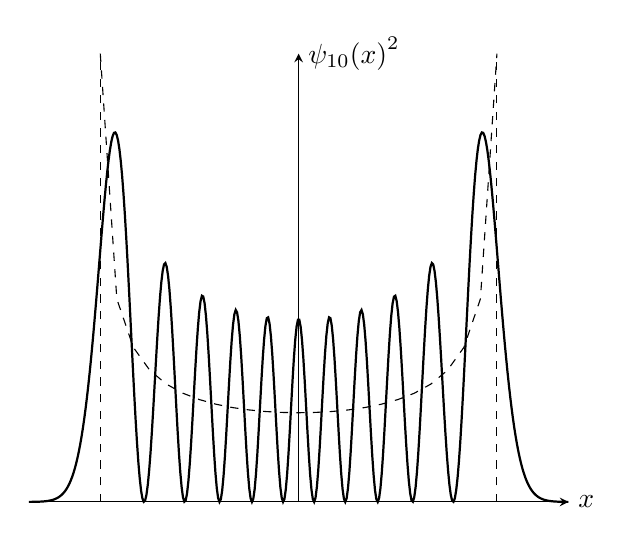
\begin{tikzpicture}[declare function={psi10(\x)=1/sqrt(2^10*3628800)*e^(-0.5*\x^2)*(1024*\x^10-23040*\x^8+161280*\x^6-403200*\x^4+302400*\x^2-30240);cl(\x)=1/sqrt(1-\x^2);}]
\begin{axis}[clip=false,axis lines=middle,xtick={\empty},ytick={\empty},xlabel={$x$},ylabel={$\abs{\psi_{10}(x)}^2$},xlabel style={at={(current axis.right of origin)},anchor=west},ylabel style={at={(current axis.above origin)},anchor=west}]
\pgfmathsetmacro{\pk}{0.12*cl(0.98)}
\addplot[thick,domain=-6:6,samples=400]{(psi10(x))^2};
\addplot[dashed,domain=-0.98:0.98]({4.5*x},{0.12*cl(x)});
\addplot[dashed] plot coordinates {(-0.98*4.5,0)(-0.98*4.5,\pk)};
\addplot[dashed] plot coordinates {(0.98*4.5,0)(0.98*4.5,\pk)};
\end{axis}
\end{tikzpicture}
\caption{}
\end{subfigure}%
\caption{ہارمونی مرتعش کے ابتدائی چار ساکن حالات۔}
\label{شکل_غیر_تابع_ہارمونی_مرتعش_ابتدائی_ساکن_حالات}
\end{figure}

\ابتدا{سوال}\شناخت{سوال_شروڈنگر_ہارمونی_مرتعش_حیطہ}
ہارمونی مرتعش کے زمینی حال میں کلاسیکی اجازتی خطہ کے باہر ایک ذرہ کی موجودگی کا احتمال (تین با معنی ہندسوں تک) تلاش کریں۔
\ترچھا{اشارہ:} کلاسیکی طور پر ایک مرتعش کی توانائی \عددی{E=(1/2)ka^{2}=(1/2)m\omega^{2}a^{2}} ہو گی جہاں \عددی{a} حیطہ ہے۔ یوں توانائی \عددی{E} کے مرتعش کا "کلاسیکی اجازتی خطا" \عددی{-\sqrt{2E/m\omega^{2}}} تا \عددی{+\sqrt{2E/m\omega^{2}}} ہو گا۔ تکمل کی قیمت "عمومی تقسیم" یا "تفاعل خلل" کی جدول سے دیکھیں۔
\انتہا{سوال}
%
\ابتدا{سوال}
کلیہ توالی (مساوات \حوالہ{مساوات_شروڈنگر_کلیہ_توالی_اجازتی_الف}) استعمال کر کے \عددی{H_{5}(\xi)} اور \عددی{H_{6}(\xi)}
تلاش کریں۔ مجموعی مستقل تعین کرنے کی خاطر \عددی{\xi} کی بلند تر طاقت کا عددی سر روایت کے تحت \عددی{2^{n}} لیں۔
\انتہا{سوال}
%
\ابتدا{سوال}\شناخت{سوال_شروڈنگر_ہرمائٹ_کثیر_رکنیاں} 
اس سوال میں ہم ہرمائٹ کثیر رکنی کے چند اہم مسائل، جن کا ثبوت پیش نہیں کیا جائے گا، پر غور کرتے ہیں۔
\begin{enumerate}[a.]
\item
\اصطلاح{کلیہ روڈریگیس}\فرہنگ{کلیہ!روڈریگیس}\حاشیہب{Rodrigues formula}\فرہنگ{Rodrigues!formula} درج ذیل کہتا ہے۔
\begin{align}
H_{n}(\xi)=(-1)^{n}e^{\xi^{\,2}}\frac{\dif^{\,n} }{\dif \xi^{\,n}}e^{-\xi^{2}}
\end{align}
اس کو استعمال کر کے \عددی{H_{3}} اور \عددی{H_{4}} اخذ کریں۔
\item
درج ذیل کلیہ توالی گزشتہ دو ہرمائٹ کثیر رکنیوں کی صورت میں \عددی{H_{n+1}} دیتا ہے۔
\begin{align}
H_{n+1}(\xi)=2\xi H_{n}(\xi)-2nH_{n-1}(\xi)
\end{align}
اس کو جزو-ا کے نتائج کے ساتھ استعمال کر کے \عددی{H_{5}} اور \عددی{H_{6}} تلاش کریں۔
\item
اگر آپ \عددی{n} رتبی کثیر رکنی کا تفرق لیں تو آپکو \عددی{n-1} رتبی کثیر رکنی حاصل ہو گی۔ ہرمائٹ کثیر رکنیوں کے لیے درج ذیل ہو گا
\begin{align}
\frac{\dif{H_{n}}}{\dif{\xi}}=2nH_{n-1}(\xi)
\end{align}
جس کی تصدیق ہرمائٹ کثیر رکنی \عددی{H_{5}} اور \عددی{H_{6}} کے لئے کریں۔ 
\item
\اصطلاح{پیداکار تفاعل}\فرہنگ{پیداکار!تفاعل}\حاشیہب{generating function}\فرہنگ{generating!function} \عددی{e^{-z^{2}+2z\xi}} کا \عددی{z=0} پر \عددی{n} واں تفرق \عددی{H_{n}(\xi)} ہو گا، یا دوسرے لفظوں میں، درج ذیل تفاعل کے ٹیلر  توسیع  میں یہ
\عددی{z^{n}/n!} کا عددی سر ہو گا۔
\begin{align}
e^{-z^{2}+2z\xi}=\sum_{n=0}^{\infty}\frac{z^{n}}{n!}H_{n}(\xi)
\end{align}
اس کو استعمال کر کے\عددی{H_0}، \عددی{H_1} اور \عددی{H_{2}} دوبارہ اخذ کریں۔
\end{enumerate}
\انتہا{سوال}
%=================================

\حصہ{آزاد ذرہ}
ہم اب آزاد ذرہ (جس کے لیے پر جگہ \عددی{V(x)=0} ہو گا) پر غور کرتے ہیں جس سادہ ترین صورت ہونی چاہیے تھی۔ کلاسیکی طور پر اس سے مراد مستقل سمتی رفتار ہو گی، لیکن کوانٹم میکانیات میں یہ مسئلہ حیران کن حد تک پیچیدہ اور پراسرار ثابت ہوتا ہے۔ غیر تابع وقت شروڈنگر مساوات ذیل 
\begin{align}\label{مساوات_شروڈنگر_آزاد_ذرہ_الف}
-\frac{\hslash^{2}}{2m}\frac{\dif^{\,2}{\psi}}{\dif{x^{2}}}=E\psi
\end{align}
یا ذیل ہے۔
\begin{align}
\frac{\dif^{\,2}{\psi}}{\dif{x^{2}}}&=-k^{\,2}\psi&& k\equiv\frac{\sqrt{2mE}}{\hslash}
\end{align}
یہاں تک یہ لامتناہی چوکور کنویں  (مساوات \حوالہ{مساوات_شروڈنگر_کلاسیکی_ہارمونی_مرتعش}) کی مانند ہے جہاں (بھی) مخفی قوہ صفر ہے؛ البتہ اس بار، میں عمومی مساوات کو قوت نما (نا کہ سائن اور کوسائن) کی صورت میں لكهنا چاہوں گا، جس کی وجہ آپ پر جلد عیاں ہو گی۔
\begin{align}
\psi(x)=Ae^{ikx}+Be^{-ikx}
\end{align}
لامتناہی چوکور کنویں  کے برعکس، یہاں کوئی سرحدی شرائط نہیں پائے جاتے ہیں جو \عددی{k} (اور یوں \عددی{E}) کی ممکنہ قیمتوں پر کسی قسم کی پابندی عائد کرتے ہوں؛ لہٰذا آزاد ذرہ کسی بھی (مثبت) توانائی کا حامل ہو سکتا ہے۔ اس کے ساتھ تابعیت وقت \عددی{e^{-iEt/\hslash}}
جوڑتے ہوئے ذیل حاصل ہو گا۔
\begin{align}\label{مساوات_شروڈنگر_آزاد_ذرہ_حرکت}
\Psi(x,t)=Ae^{ik(x-\frac{\hslash k}{2m}t)}+Be^{-ik(x+\frac{\hslash k}{2m}t)}
\end{align}
ایسا کوئی بھی تفاعل جو \عددی{x} اور \عددی{t} متغیرات کی مخصوص جوڑ \عددی{(x\pm vt)} کا تابع ہو (جہاں \عددی{v} مستقل ہے)، 
 غیر تغیر شکل و صورت کی ایسی موج کو ظاہر کرے گا جو \عددی{v} رفتار سے \عددی{\mp x} رخ حرکت کرتی ہے۔ اس موج پر ایک اٹل نقطہ (مثلاً کم سے کم یا زیادہ سے زیادہ قیمت کا نقطہ) تفاعل کے \اصطلاح{دلیل}\فرہنگ{دلیل}\حاشیہب{argument}\فرہنگ{argument} کی ایک اٹل قیمت کا یوں مطابقتی ہو گا کہ درج ذیل ہو۔
\begin{align*}
x=\mp vt+\text{مستقل}\quad \text{یا}\quad x\pm vt=\text{مستقل}
\end{align*}
چونکہ موج پر تمام نقاط ایک جیسی سمتی رفتار سے حرکت کرتے ہیں لہٰذا موج کی شکل و صورت حرکت کے ساتھ تبدیل نہیں ہو گی۔ یوں مساوات \حوالہ{مساوات_شروڈنگر_آزاد_ذرہ_حرکت} کا پہلا جزو دائیں رخ حرکت کرتی موج کو ظاہر کرتا ہے جبکہ اس کا دوسرا جزو بائیں رخ حرکت کرتی (اتنی ہی توانائی کی) موج کو ظاہر کرتا ہے۔ چونکہ ان میں فرق صرف \عددی{k} کی علامت کا ہے لہٰذا انہیں درج ذیل بھی لکھا جا سکتا ہے 
\begin{align}\label{مساوات_غیر_تابع_دائیں_رخ_چلتی}
\Psi_{k}(x,t)=Ae^{i(kx-\frac{\hslash k^{2}}{2m}t)}
\end{align}
جہاں \عددی{k} کی قیمت منفی لینے سے بائیں رخ حرکت کرتی موج حاصل ہو گی۔
\begin{align}
k\equiv \pm\frac{\sqrt{2mE}}{\hslash},\quad
\begin{cases}
k>0\Rightarrow \text{\RL{دائیں رخ حرکت}}\\
k<0\Rightarrow \text{\RL{بائیں رخ حرکت}}
\end{cases}
\end{align}
صاف ظاہر ہے کہ آزاد ذرے کے "ساکن حالات" حرکت کرتی امواج کو ظاہر کرتے ہیں، جن کی طول موج \عددی{\lambda=2\pi/\abs{k}} ہو گا، اور کلیہ ڈی بروگ لی (مساوات \حوالہ{مساوات_تفاعل_موج_ڈی_بروگلی_معیار_حرکت}) کے تحت ان کا معیار حرکت درج ذیل ہو گا۔
\begin{align}\label{مساوات_غیر_تابع_ڈی_براگلی_معیار_حرکت}
p=\hslash k
\end{align}
ان امواج کی رفتار (یعنی \عددی{t} کا عددی سر تقسیم \عددی{x} کا عددی سر) درج ذیل ہو گا۔
\begin{align}
v_{\text{کوانٹائی}}=\frac{\hslash\abs{k}}{2m}=\sqrt{\frac{E}{2m}}
\end{align}
اس کے برعکس ایک آزاد ذرہ جس کی توانائی \عددی{E} ہو (جو خالصتاً حرکی ہو گی چونکہ \عددی{V=0} ہے) کی کلاسیکی رفتار \عددی{E=(1/2)mv^{2}} سے حاصل کی جا سکتی ہے۔
\begin{align}\label{مساوات_شروڈنگر_کلاسیکی_کوانٹائی_رفتار}
v_{\text{کلاسیکی}}=\sqrt{\frac{2E}{m}}=2v_{\text{کوانٹائی}}
\end{align}
ظاہری طور پر کوانٹم میکانی تفاعل موج اس ذرے کی نصف رفتار سے حرکت کرتا ہے جس کو یہ ظاہر کرتا ہے۔ اس تضاد پر ہم کچھ دیر میں غور کریں گے۔ اس سے پہلے ایک زیادہ سنگین مسئلہ پر غور کرنا ضروری ہے۔ درج ذیل کے تحت یہ تفاعل موج معمول پر لانے کے قابل نہیں ہے۔ 
\begin{align}
\int_{-\infty}^{+\infty}\Psi_{k}^{*}\Psi_{k}\dif{x}=\abs{A}^{2}\int_{-\infty}^{+\infty}\dif{x}=\abs{A}^{2}(\infty)
\end{align}
یوں آزاد ذرے کی صورت میں قابل علیحدگی حل طبیعی طور پر قابل قبول حالات کو ظاہر نہیں کرتے ہیں۔ ایک آزاد ذرہ ساکن حال میں نہیں پایا جا سکتا ہے؛ دوسرے لفظوں میں، غیر مبہم توانائی کے ایک آزاد ذرے کا تصور بے معنی ہے۔

 اس کا ہرگز یہ مطلب نہیں کہ قابل علیحدگی حل ہمارے کسی کام کے نہیں ہیں، کیونکہ یہ طبیعی مفہوم سے آزاد، ریاضیاتی کردار ادا کرتے ہیں۔ تابع وقت شروڈنگر مساوات کا عمومی حل اب بھی قابل علیحدگی حلوں کا خطی جوڑ ہو گا (صرف اتنا ہے کہ غیر مسلسل اشاریہ \عددی{n} پر مجموعہ کی بجائے اب یہ استمراری متغیر \عددی{k} کے لحاظ سے تکمل ہو گا)۔
\begin{align}\label{مساوات_غیر_تابع_استمراری_شروڈنگر_حل}
\Psi(x,t)=\frac{1}{\sqrt{2\pi}}\int_{-\infty}^{+\infty}\phi(k)e^{i(kx-\frac{\hslash k^{2}}{2m}t)}\dif{k}
\end{align}


(ہم \عددی{ \frac{1}{\sqrt{2 \pi }} } کو اپنی آسانی کیلئے تکمل کے باہر نکالتے ہیں؛ مساوات 
 \حوالہ{مساوات_شروڈنگر_عمومی_حل_مجموعہ} میں عددی سر \عددی{ c_{n} } کی جگہ یہاں \عددی{ ( 1/\sqrt{2\pi}) \phi(k) \dif k } کردار ادا کرتا ہے۔) اب اس تفاعل موج کو (موزوں \عددی{ \phi(k) } کیلئے) معمول پر لایا جا سکتا ہے۔ تاہم اس میں \عددی{k} کی قیمتوں کی سعت پائی جائے گی، لہٰذا توانائیوں اور رفتاروں کی بھی سعت پائی جائیں گی۔ ہم اس کو \اصطلاح{موجی اکٹھ}\فرہنگ{موجی اکٹھ}\حاشیہب{wave packet}\فرہنگ{wave!packet} کہتے ہیں۔\حاشیہد{سائن نما امواج کی وسعت لامتناہی تک پہنچتی ہے اور یہ معمول پر لانے کے قابل نہیں ہوتی ہیں۔ تاہم ایسی امواج کا خطی میل تباہ کن مداخلت پیدا کرتا ہے، جس کی بنا پر مقام بندی اور معمول زنی ممکن ہوتی ہے۔}

عمومی کوانٹم مسئلہ میں ہمیں \عددی{ \Psi (x,0) } فراہم کر کے \عددی{ \Psi(x,t) } تلاش کرنے کو کہا جاتا ہے۔ آزاد ذرے کیلئے اس کا حل مساوات \حوالہ{مساوات_غیر_تابع_استمراری_شروڈنگر_حل} کی صورت اختیار کرتا ہے۔ اب سوال یہ پیدا ہوتا ہے کہ ابتدائی تفاعل موج 
\begin{align}
\Psi (x,0) = \frac{1}{\sqrt{2\pi}} \int_{- \infty}^{+ \infty} \phi (k) e^{ikx} \dif k
\end{align}
پر پورا اترتا ہوا \عددی{ \psi(k) } کیسے تعین کیا جائے؟ یہ فوریئر تجزیہ کا کلاسیکی مسئلہ ہے جس کا جواب \اصطلاح{مسئلہ پلانشرال:}\فرہنگ{مسئلہ!پلانشرال}\حاشیہب{Plancherel's theorem}\فرہنگ{theorem!Plancherel}
\begin{align}\label{مساوات_شروڈنگر_مسئلہ_پلانشرل}
f(x) = \frac{1}{\sqrt{2\pi}} \int_{- \infty}^{+ \infty} F(k) e^{ikx} \dif k \Leftrightarrow F(k) = \frac{1}{\sqrt{2\pi}} \int_{- \infty}^{+ \infty} f(x) e^{-ikx} \dif x
\end{align}
 پیش کرتا ہے (سوال \حوالہ{سوال_غیر_تابع_پلانشرال_ثبوت_مدد} دیکھیں)۔ \عددی{F(k)} کو \عددی{f(x)} کا \اصطلاح{فوریئر بدل}\فرہنگ{فوریئر!بدل}\حاشیہب{Fourier transform}\فرہنگ{Fourier!transform} کہا جاتا ہے جبکہ \عددی{f(x)} کو \عددی{F(k)} کا \اصطلاح{الٹ فوریئر بدل}\فرہنگ{فوریئر!الٹ بدل}\حاشیہب{inverse Fourier transform}\فرہنگ{Fourier!inverse transform} کہتے ہیں (ان دونوں میں صرف قوت نما کی علامت کا فرق پایا جاتا ہے)۔ ہاں، اجازتی تفاعل پر کچھ پابندی ضرور عائد ہے: تکمل کا \ترچھا{موجود}\حاشیہد{تفاعل \عددی{f(x)} پر عائد لازم اور کافی پابندی یہ ہے کہ \عددی{\int_{-\infty}^{\infty}\abs{f(x)}^2\dif x} متناہی ہو۔ (ایسی صورت میں \عددی{\int_{-\infty}^{\infty}\abs{F(k)}^2\dif k} بھی متناہی ہو گا، اور حقیقتاً ان دونوں تکملات کی قیمتیں ایک  جتنی ہوں گی۔ \text{Arfken} کے حصہ \text{15.5} میں حاشیہ \text{24} دیکھیں۔)}\شناخت{حاشیہ_شروڈنگر_مربع_تکملیت} ہونا لازم ہے۔ ہمارے مقاصد کے لئے، تفاعل \عددی{\Psi(x,0)} پر بذات خود معمول شدہ ہونے کی طبیعی شرط مسلط کرنا اس کی ضمانت دے گا۔ یوں آزاد ذرے کے عمومی کوانٹم مسئلہ کا حل مساوات \حوالہ{مساوات_غیر_تابع_استمراری_شروڈنگر_حل} ہو گا جہاں \عددی{\phi(k)} درج ذیل ہو گا۔ 
\begin{align}\label{مساوات_شروڈنگر_الٹ_بدل_سائے}
\phi(k) = \frac{1}{\sqrt{2\pi}} \int_{- \infty}^{+\infty} \Psi(x,0)e^{-ikx} \dif x
\end{align}
%===============
\ابتدا{مثال}\شناخت{مثال_غیر_تابع_مستطیل_کچھ_دیر_بعد}
ایک آزاد ذرہ جو ابتدائی طور پر خطہ \عددی{ -a \leq x \leq a } میں رہنے کا پابند ہو کو وقت \عددی{t=0} پر چھوڑ دیا جاتا ہے:
\begin{align*}
\Psi (x,0) =
\begin{cases}
A, & -a < x < a,\\
 0, &\text{\RL{دیگر صورت}}
\end{cases}
\end{align*}
جہاں \عددی{ A } اور \عددی{ a } مثبت حقیقی مستقل ہیں۔ \عددی{ \Psi(x,t) } تلاش کریں۔ 

حل: \quad
ہم پہلے \عددی{ \Psi(x,0) } کو معمول پر لاتے ہیں۔ 
\begin{align*}
1 = \int_{-\infty}^{\infty} \left| \Psi (x,0) \right| ^{2} \dif x = \left| A \right|^{2} \int_{-a}^{a} \dif x = 2a \left| A \right|^{2} \Rightarrow A = \frac{1}{\sqrt{2a}}
\end{align*}
اس کے بعد مساوات \حوالہ{مساوات_شروڈنگر_الٹ_بدل_سائے} استعمال کرتے ہوئے \عددی{ \psi(k) } تلاش کرتے ہیں۔
\begin{align*}
\phi(k) =& \frac{1}{\sqrt{2\pi}} \frac{1}{\sqrt{2a}} \int_{-a}^{a} e^{-ikx} \dif x = \frac{1}{2\sqrt{\pi a}} \left. \frac{e^{-ikx}}{-ik} \right|_{-a}^{a} \\
=& \frac{1}{k\sqrt{\pi a}} \left( \frac{e^{ikx} - e^{-ikx}}{2i} \right) = \frac{1}{\sqrt{\pi a}} \frac{\sin(ka)}{k}
\end{align*}
آخر میں ہم اس کو دوبارہ مساوات \حوالہ{مساوات_غیر_تابع_استمراری_شروڈنگر_حل} میں پر کرتے ہیں۔ 
\begin{align}\label{مساوات_غیر_تابع_مستطیل_سے_ارتقا_مشکل_ہے}
\Psi (x,t) = \frac{1}{\pi \sqrt{2a}} \int_{-\infty}^{\infty} \frac{\sin (ka)}{k} e^{i(kx-\frac{\hslash k^{2}}{2m}t)} \dif k
\end{align}
بد قسمتی سے اس تکمل کو بنیادی تفاعل کی صورت میں حل کرنا ممکن نہیں ہے، تاہم اس کی قیمت کو اعدادی تراکیب سے حاصل کیا جا سکتا ہے (شکل \حوالہ{شکل_غیر_تابع_مستطیل_سے_ارتقا})۔ (ایسی بہت کم صورتیں حقیقتاً پائی جاتی ہیں جن کے لئے \عددی{\Psi(x,t)} کا 
تکمل (مساوات \حوالہ{مساوات_غیر_تابع_استمراری_شروڈنگر_حل}) صریحاً حل کرنا ممکن ہو۔ سوال \حوالہ{سوال_شروڈنگر_گاوسی_موجی_اکٹھ} میں ایسی ایک بالخصوص خوبصورت مثال پیش کی گئی ہے۔)

\begin{comment}
the evolution of a rectangular wave function (fig 2.8, p75) is produced by the octave code "./tex/octave/evolutionFromRectangular.m" reproduced below. this code produces the table "evolutionFromRectangular.dat" which must be placed in the folder "./tex/tables/" (as specified by "\pgfplotsset{table/search path={./tex/tables},}" in the preamble).

"evolutionFromRectangular.m"
{
clear;
clf;
%
for i=1:100
a=1;
f=@(k) 1/(pi*sqrt(2*a))*sin(k*a)./k.*cos(k.*(0.12*i-6)-k.^2*a^2/2);
g=@(k) 1/(pi*sqrt(2*a))*sin(k*a)./k.*sin(k.*(0.12*i-6)-k.^2*a^2/2);
psiSquared(i)=(quadgk(f,-30,30))^2+(quadgk(g,-30,30))^2;
endfor
%
i=1:100;
plot(i,psiSquared(i));
%
khorcat=rot90([psiSquared;0.12*i-6],-1);
%
kkk=fopen("evolutionFromRectangular.dat","w");
fdisp(kkk,khorcat)
fclose(kkk);
}
\end{comment}
%
\begin{figure}
\centering
\begin{tikzpicture}
\begin{axis}[small,axis lines=middle,xlabel={$\frac{x}{a}$},ylabel={$\abs{\Psi(x,t)}^2$},xlabel style={at={(current axis.right of origin)},anchor={west}},enlargelimits,,ylabel style={at={(current axis.above origin)},anchor=west},ytick={\empty},yticklabels={$0.1$,$0.2$,$0.3$,$0.4$,$0.5$},extra y tick style={y tick label style={left, xshift=-1.5ex}}, extra y ticks={0.1,0.2,0.3,0.4,0.5}]
\addplot[black,thick] table[x index=0,y index=1,smooth,mark=none] {evolutionFromRectangular.dat};
\addplot[black,thick]plot coordinates{(-1,0)(-1,0.5)(1,0.5)(1,0)};
\end{axis}
\end{tikzpicture}
\caption{
تفاعل \عددی{\abs{\Psi(x,t)}^2} کی لمحہ \عددی{t=0}پر مستطیل اور \عددی{t=ma^2/\hslash} پر قوسی ترسیم (مساوات \حوالہ{مساوات_غیر_تابع_مستطیل_سے_ارتقا_مشکل_ہے})۔
}
\label{شکل_غیر_تابع_مستطیل_سے_ارتقا}
\end{figure}

 \begin{figure}
\centering
\begin{subfigure}{0.45\textwidth}
\centering
\begin{tikzpicture}
\begin{axis}[small,axis lines=middle,xlabel={$x$},ylabel={$\Psi(x,0)$},xtick={\empty},ytick={\empty},xlabel style={at={(current axis.right of origin)},anchor=north},ylabel style={at={(current axis.above origin)},anchor=west},enlargelimits]
\addplot[thick] plot coordinates {(-2,0)(-0.2,0)(-0.2,1)(0.2,1)(0.2,0)(2,0)};
\addplot[]plot coordinates {(-0.2,1)}node[left]{$\frac{1}{\sqrt{2a}}$};
\addplot[]plot coordinates {(-0.2,0)}node[below,xshift=-5pt]{$-a$};
\addplot[]plot coordinates {(0.2,0)}node[below]{$a$};
\end{axis}
\end{tikzpicture}
\caption{}
\end{subfigure}\hfill
\begin{subfigure}{0.45\textwidth}
\centering
\begin{tikzpicture}
\begin{axis}[small,axis lines=middle,xlabel={$k$},ylabel={$\phi(k)$},xtick={\empty},ytick={\empty},xlabel style={at={(current axis.right of origin)},anchor=north},ylabel style={at={(current axis.above origin)},anchor=west},enlargelimits,ymin=0,ymax=1]
\addplot[thick] plot coordinates {(-2,0.1)(2,0.1)}node[pos=0.5,above right]{$\sqrt{a/\pi}$};
\end{axis}
\end{tikzpicture}
\caption{}
\end{subfigure}
\caption{
چھوٹے \عددی{a} کے لئے مثال \حوالہ{مثال_غیر_تابع_مستطیل_کچھ_دیر_بعد}۔ (ا) \عددی{\Psi(x,0)} کی ترسیم؛ (ب) \عددی{\phi(k)} کی ترسیم۔
}
\label{شکل_غیر_تابع_مستطیل_کچھ_دیر_بعد}
\end{figure}

آئیں ایک تحدیدی صورت پر غور کریں۔ اگر \عددی{a} کی قیمت بہت کم ہو تب ابتدائی تفاعل موج خوبصورت مقامی نوکیلی صورت اختیار کرتی ہے (شکل \حوالہ{شکل_غیر_تابع_مستطیل_کچھ_دیر_بعد}-ا)۔ ایسی صورت میں ہم چھوٹے زاویوں کے لئے تخمیناً \عددی{ \sin ka \approx ka } لکھ کر درج ذیل حاصل کرتے ہیں
\begin{align*}
\phi (k) \approx \sqrt{\frac{a}{\pi}}
\end{align*}
جو \عددی{k} کی مختلف قیمتوں کا آپس میں کٹ جانے کی بنا پر افقی ہے (شکل \حوالہ{شکل_غیر_تابع_مستطیل_کچھ_دیر_بعد}-ب)۔ یہ مثال ہے اصول عدم یقینیت کی: اگر ذرے کے مقام میں وسعت  کم ہو، تب اس کی معیار حرکت (لہٰذا \عددی{k}، مساوات \حوالہ{مساوات_غیر_تابع_ڈی_براگلی_معیار_حرکت} دیکھیں) کی وسعت  لازماً زیادہ ہو گا۔ اس کی دوسری انتہا (بڑی \عددی{a}) کی صورت میں مقام کی وسعت و زیادہ ہو گی  (شکل \حوالہ{شکل_غیر_تابع_بڑا_اے_سائے_فائے}) لہٰذا درج ذیل ہو گا۔ 
\begin{align*}
\phi (k) = \sqrt{\frac{a}{\pi}} \frac{\sin ka }{ka }
\end{align*}

\begin{figure}
\centering
\begin{subfigure}{0.45\textwidth}
\centering
\begin{tikzpicture}
\begin{axis}[small,axis lines=middle,xlabel={$x$},ylabel={$\Psi(x,0)$},xtick={\empty},xlabel style={at={(current axis.right of origin)},anchor={north}},enlargelimits,ytick={\empty},ylabel style={at={(current axis.above origin)},anchor=north west},ymax=5]
\addplot[thick]plot coordinates {(-4,1)(4,1)}node[pos=0.5,above right]{$\frac{1}{\sqrt{2a}}$};
\end{axis}
\end{tikzpicture}
\caption{}
\end{subfigure}\hfill
\begin{subfigure}{0.45\textwidth}
\centering
\pgfmathsetmacro{\a}{1}
\pgfmathsetmacro{\kx}{3.5*pi/\a}
\pgfmathsetmacro{\kxA}{pi/\a}
\pgfmathsetmacro{\ky}{sqrt(\a/pi)}
\begin{tikzpicture}[declare function={kphi(\k)=sqrt(\a/pi)*sin(deg(\k*\a))/(\k*\a);}]
\begin{axis}[small,axis lines=middle,xlabel={$k$},ylabel={$\phi(k)$},xlabel style={at={(current axis.right of origin)},anchor={north}},enlargelimits,ytick={\ky},yticklabels={$\sqrt{\frac{a}{\pi}}$},ylabel style={at={(current axis.above origin)},anchor=west},xtick={-\kxA,\kxA},xticklabels={$-\frac{\pi}{a}$,$\frac{\pi}{a}$}]
\addplot[thick,domain=-0.01:-\kx,variable=\k,smooth] {kphi(k)};
\addplot[thick,domain=0.01:\kx,variable=\k,smooth] {kphi(k)};
\end{axis}
\end{tikzpicture}
\caption{}
\end{subfigure}
\caption{
بڑی \عددی{a} کے لئے (ا) \عددی{\Psi(x,0)} کی ترسیم، (ب) \عددی{\phi(k)} کی ترسیم (مثال \حوالہ{مثال_غیر_تابع_مستطیل_کچھ_دیر_بعد})۔
}
\label{شکل_غیر_تابع_بڑا_اے_سائے_فائے}
\end{figure}
اب \عددی{ \sin z/z } کی زیادہ سے زیادہ قیمت \عددی{ z=0 } پر پائی جاتی ہے جو گھٹ کر \عددی{ z=\pm\pi } ( جو یہاں \عددی{ k=\pm \pi/a } کو ظاہر کرتا ہے) پر صفر ہوتی ہے۔ یوں بڑی \عددی{ a } کیلئے \عددی{ k=0 } پر \عددی{\phi (k)} نوکیلی صورت اختیار کرے گا (شکل \حوالہ{شکل_غیر_تابع_بڑا_اے_سائے_فائے})۔ اس بار ذرے کی معیار حرکت اچھی طرح معین ہے جبکہ اس کا مقام صحیح طور پر معلوم نہیں ہے۔
\انتہا{مثال}
%=================
آئیں اب اس تضاد پر دوبارہ بات کریں جس کا ذکر ہم پہلے کر چکے: جہاں مساوات \حوالہ{مساوات_غیر_تابع_دائیں_رخ_چلتی} میں دیا گیا علیحدگی حل \عددی{\Psi_{k} (x, t)}، ٹھیک اس ذرہ کی رفتار سے حرکت نہیں کرتی ہے جس کو یہ بظاہر ظاہر کرتی ہے۔ حقیقتاً یہ مسئلہ وہیں پر ختم ہو گیا تھا جب ہم جان چکے کہ \عددی{\Psi_{k}} طبیعی طور پر قابل حصول حل نہیں ہے۔ بحر حال آزاد ذرے کی تفاعل موج (مساوات \حوالہ{مساوات_غیر_تابع_استمراری_شروڈنگر_حل}) میں سموئی سمتی رفتار کی معلومات پر غور کرنا دلچسپی کا باعث ہے۔ بنیادی تصور کچھ یوں ہے: سائن نما تفاعلات کا خطی میل جس کے حیطہ کو \عددی{\phi} ترمیم کرتا ہو (شکل \حوالہ{شکل_غیر_تابع_موجی_اکٹھ_رفتاریں}) موجی اکٹھ ہو گا؛ یہ "غلاف" میں ڈھانکے ہوئے "لہروں" پر مشتمل ہو گا۔ انفرادی لہر کی رفتار، جس کو \اصطلاح{دوری سمتی رفتار}\فرہنگ{رفتار!دوری سمتی}\حاشیہب{phase velocity}\فرہنگ{velocity!phase} \عددی{(v_p)} کہتے ہیں، ہرگز ذرے کی سمتی رفتار کو ظاہر نہیں کرتی ہے بلکہ غلاف کی رفتار، جس کو \اصطلاح{گروہی سمتی رفتار}\فرہنگ{رفتار!گروہی سمتی}\حاشیہب{group velocity}\فرہنگ{velocity!group} \عددی{(v_g)}کہتے ہیں، ذرے کی رفتار ہو گی۔ غلاف کی سمتی رفتار لہروں کی فطرت پر منحصر ہو گی؛ یہ لہروں کی سمتی رفتار سے زیادہ، کم یا اس کے برابر ہو سکتی ہے۔ ایک دھاگے پر امواج کی گروہی سمتی رفتار اور دوری سمتی رفتار  برابر ہوتی ہیں۔ پانی کی امواج کیلئے یہ دوری سمتی رفتار کی نصف ہو گی، جیسا آپ نے جھیل میں پتھر پھینک کر دیکھا ہو گا (اگر آپ پانی کی ایک مخصوص لہر پر نظر جمائے رکھیں تو آپ دیکھیں گے کہ، پیچھے سے آگے کی طرف بڑھتے ہوئے، آغاز میں اس لہر کا حیطہ بڑھتا ہے جبکہ آخر میں آگے پہنچ کر اس کا حیطہ گھٹ کر صفر ہو جاتا ہے؛ اس دوران یہ تمام بطور ایک مجموعہ نصف رفتار سے حرکت کرتا ہے۔) یہاں میں نے دکھانا ہو گا کہ کوانٹم میکانیات میں آزاد ذرے کے تفاعل موج کی گروہی سمتی رفتار اس کی دوری سمتی رفتار سے دگنی ہے، جو عین ذرے کی کلاسیکی رفتار ہے۔

\begin{figure}
\centering
\pgfmathsetmacro{\ka}{1}
\pgfmathsetmacro{\kb}{10}
\pgfmathsetmacro{\kc}{157}
\pgfmathsetmacro{\kd}{140}
\begin{tikzpicture}[declare function={kp(\x)=(1.5+sin(\ka*\x))*sin(\kb*\x);kg(\x)=1.5+sin(\ka*\x);}]
\begin{axis}[small,axis lines=middle,xlabel={$x$},ylabel={\empty},xlabel style={at={(current axis.right of origin)},anchor={north}},enlargelimits,ytick={\empty},ylabel style={at={(current axis.above origin)},anchor=west},xtick={\empty}]
\addplot[thick,domain=-30:400,samples=1000] {kp(x)};
\addplot[thick,domain=-30:400,samples=1000] {kg(x)};
\addplot[thick,domain=-30:400,samples=1000] {-kg(x)};
\addplot[-stealth] plot coordinates {(\kc,{kp(\kc)})({\kc+100},{kp(\kc)})}node[right]{$v_p$};
\addplot[-stealth] plot coordinates {(\kd,{kg(\kd)})({\kd+117},{kg(\kd)})}node[right]{$v_g$};
\end{axis}
\end{tikzpicture}
\caption{موجی اکٹھ۔" غلاف" گروہی سمتی رفتار جبکہ لہر دوری سمتی رفتار سے حرکت کرتی ہے۔}
\label{شکل_غیر_تابع_موجی_اکٹھ_رفتاریں}
\end{figure}
 ہمیں درج ذیل عمومی صورت کے موجی اکٹھ کی گروہی سمتی رفتار تلاش کرنی ہو گی۔ 
\begin{align*}
\Psi (x,t) = \frac{1}{\sqrt{2\pi}} \int_{- \infty}^{+ \infty} \phi (k) e^{i(kx - \omega t)} \dif k
\end{align*}
 (یہاں \عددی{\omega = (\hslash k^{2} /2m)} ہے، لیکن جو کچھ میں کہنے جا رہا ہوں وہ کسی بھی موجی اکٹھ کیلئے، اس کے \اصطلاح{انتشاری رشتہ}\فرہنگ{انتشاری!رشتہ}\حاشیہب{dispersion relation}\فرہنگ{dispersion!relation} (\عددی{\omega} کا متغیر \عددی{k} کے لحاظ سے کلیہ) سے قطع نظر، درست ہو گا۔) ہم فرض کرتے ہیں کہ کسی مخصوص قیمتی \عددی{k_{0}} پر \عددی{\phi (k)} نوکیلی صورت اختیار کرتا ہے۔ (ہم زیادہ وسعت کا \عددی{k} بھی لے سکتے ہیں لیکن ایسے موجی اکٹھ کے مختلف اجزاء مختلف رفتار سے حرکت کرتے ہیں جس کی بنا پر یہ موجی اکٹھ بہت تیزی سے اپنی شکل و صورت تبدیل کرتا ہے اور کسی مخصوص سمتی رفتار پر حرکت کرتے ہوئے ایک مجموعہ کا تصور بے معنی ہو جاتا ہے۔) چونکہ \عددی{k_{0}} سے دور متکمل قابل نظر انداز ہے لہٰذا ہم تفاعل \عددی{\omega (k)} کو اس نقطہ کے گرد ٹیلر تسلسل سے پھیلا کر صرف ابتدائی اجزاء لیتے ہیں:
\begin{align*}
\omega (k) \cong \omega_{0} + \omega_{0}^{'} (k-k_{0})
\end{align*}
 جہاں نقطہ \عددی{k_{0}} پر \عددی{k} کے لحاظ سے \عددی{\omega} کا تفرق \عددی{\omega_{0}^{'}} ہے۔
 
(تکمل کے وسط کو \عددی{k_{0}} پر منتقل کرنے کے غرض سے) ہم متغیر \عددی{k} کی جگہ متغیر \عددی{s=k-k_{0}} استعمال کرتے ہیں۔ یوں درج ذیل ہو گا۔ 
\begin{align*}
\Psi (x,t) \cong \frac{1}{\sqrt{2 \pi }} \int_{- \infty}^{+ \infty} \phi (k_{0} + s) e^{i[(k_{0} +s)x-(\omega_{0} + \omega_{0}^{'}s )t]} \dif s
\end{align*}
 وقت \عددی{  t=0 } پر 
\begin{align*}
\Psi (x,0) = \frac{1}{\sqrt{2 \pi }} \int_{- \infty}^{+ \infty} \phi (k_{0} + s) e^{i(k_{0} +s)x} \dif s
\end{align*}
 جبکہ بعد کے وقت پر درج ذیل ہو گا۔ 
\begin{align*}
\Psi (x,t) \cong \frac{1}{\sqrt{2 \pi}} e^{i(-\omega_{0}t+k_{0}\omega_{0}^{'}t)} \int_{-\infty}^{+\infty} \phi (k_{0} + s) e^{i(k_{0} + s ) ( x - \omega_{0}^{'}t)} \dif s
\end{align*}
 ما سوائے \عددی{x} کو \عددی{(x - \omega_{0}^{'}t)} منتقل کرنے کے یہ \عددی{\Psi(x,0)} میں پایا جانے والا تکمل ہے۔ یوں درج ذیل ہو گا۔ 
\begin{align}
\Psi(x,t) \cong e^{-i(\omega_{0} - k_{0} \omega_{0}^{'})t} \,\Psi(x-\omega_{0}^{'}t,0)
\end{align}
 ماسوائے دوری جزو ضرب کے (جو کسی بھی صورت میں \عددی{\left| \Psi \right|^{2}} کی قیمت پر اثر انداز نہیں ہو گا) یہ موجی اکٹھ بظاہر سمتی رفتار \عددی{\omega_{0}^{'}} سے حرکت کرے گا: 
\begin{align}
v_{\text{گروہی}} = \frac{\dif \omega}{\dif k}
\end{align}
 (جس کی قیمت کا حساب \عددی{k = k_{0}} پر کیا جائے گا)۔ آپ دیکھ سکتے ہیں کہ یہ دوری رفتار سے مختلف ہے جسے درج ذیل مساوات پیش کرتی ہے۔ 
\begin{align}
v_{\text{دوری}} = \frac{\omega}{k}
\end{align}
 یہاں \عددی{  \omega = (\hslash k^{2} /2m) } یعنی \عددی{ \omega/k = (\hslash k/2m) } ہے جبکہ \عددی{ \dif \omega / \dif k = (\hslash k /m) } ہے جو دگنا ہے۔ یہ اس بات کی تصدیق کرتا ہے کہ موجی اکٹھ کی گروہی سمتی رفتار نا کہ ساکن حالات کی دوری سمتی رفتار کلاسیکی ذرے کی رفتار دے گی۔ 
\begin{align}
v_{\text{کلاسیکی}} = v_{\text{گروہی}} = 2v_{\text{دوری}}
\end{align}
%=====================
\ابتدا{سوال}
دکھائیں کہ متغیر \عددی{ x } کے کسی بھی تفاعل کو لکھنے کے دو معادل طریقے \عددی{ [ Ae^{ikx}+Be^{-ikx}] } اور \عددی{ [C\cos kx + D\sin kx ] } ہیں۔ مستقلات \عددی{ C } اور \عددی{ D } کو مستقلات \عددی{ A } اور \عددی{  B } کی صورت میں لکھیں۔ اسی طرح مستقلات \عددی{ A } اور \عددی{ B } کو مستقلات \عددی{ C } اور \عددی{  D } کی صورت میں لکھیں۔ \ترچھا{تبصرہ:} کوانٹم میکانیات میں جب \عددی{  V=0 } ہو، قوت نمائی تفاعل حرکت کرتے امواج کو ظاہر کرتی ہے اور انہیں استعمال کرتے ہوئے آزاد ذرے پر تبصرہ کرنا زیادہ آسان ہوتا ہے، جبکہ \عددی{  \sin } اور \عددی{ \cos } ساکن امواج کو ظاہر کرتی ہے جو لامتناہی چوکور کنویں  میں پائی جاتی ہے۔ 
\انتہا{سوال}
%================
\ابتدا{سوال}\شناخت{سوال_شروڈنگر_احتمال_بہاو_رو}
مساوات \حوالہ{مساوات_غیر_تابع_دائیں_رخ_چلتی} میں دی گئی آزاد ذرے کے تفاعل موج کا احتمال رو \عددی{ J} تلاش کریں (سوال \حوالہء{1.14} دیکھیں)۔ احتمال رو کے بہاو کا رخ کیا ہو گا؟
\انتہا{سوال}
%=============== 
\ابتدا{سوال}\شناخت{سوال_غیر_تابع_پلانشرال_ثبوت_مدد}
اس سوال میں آپ کو مسئلہ پلانشرال کا ثبوت حاصل کرنے میں مدد دیا جائے گا۔ آپ متناہی وقفہ کے فوریئر تسلسل سے آغاز کر کے اس وقفہ کو وسعت دیتے ہوئے لامتناہی تک بڑھاتے گے۔ 

\begin{enumerate}[a. ]
\item 
مسئلہ ڈرشلے کہتا ہے کہ وقفہ \عددی{ [-a, +a] } پر کسی بھی تفاعل \عددی{ f(x) } کو فوریئر تسلسل  توسیع  سے ظاہر کیا جا سکتا ہے:
\begin{align*}
f(x) = \sum_{n=0}^{\infty} [ a_{n}\sin( n\pi x/a ) + b_{n}\cos( n\pi x/a )]
\end{align*}
دکھائیں کہ اس کو درج ذیل معادل روپ میں بھی لکھا جا سکتا ہے۔
\begin{align*}
f(x) = \sum_{n=-\infty}^{\infty} c_{n}e^{i n \pi x /a }
\end{align*}
\عددی{ a_{n} } اور \عددی{ b_{n} } کی صورت میں \عددی{ c_{n} } کیا ہو گا ؟
 \item
 فوریئر تسلسل کے عددی سروں کے حصول کی مساواتوں سے درج ذیل اخذ کریں۔
\begin{align*}
c_{n} = \frac{1}{2a} \int_{-a}^{+a} f(x)e^{-in\pi x/a} \dif x
\end{align*}
\item
\عددی{ n } اور \عددی{ c_{ n } } کی جگہ نئے متغیرات \عددی{ k=( \tfrac{n \pi}{a}) } اور 
 \عددی{ F(k) = \sqrt{\tfrac{2}{\pi}}\,ac_{n } } استعمال کرتے ہوئے دکھائیں کہ جزو-ا اور جزو-ب درج ذیل روپ اختیار کرتے ہیں 
\begin{align*}
f(x) &= \frac{1}{\sqrt{2 \pi }} \sum_{n=-\infty}^{\infty} F(k)e^{ikx} \Delta k; && F(k) = \frac{1}{\sqrt{2\pi}} \int_{-a}^{+a} f(x) e^{-ikx} \dif x,
\end{align*}
جہاں ایک \عددی{ n } سے اگلی \عددی{ n } تک \عددی{ k } میں تبدیلی \عددی{ \Delta k } ہے۔ 
\item
حد \عددی{ a \rightarrow \infty } لیتے ہوئے مسئلہ پلانشرال حاصل کریں۔ \ترچھا{تبصرہ:} \عددی{ F(k) } کی صورت میں \عددی{ f(x) } اور \عددی{ f(x) } کی صورت میں \عددی{ F(k) } کے کلیات کے آغاز دو بالکل مختلف جگہوں ہوئیں۔ اس کے باوجود حد \عددی{ a \rightarrow \infty } کی صورت میں ان دونوں کی ساخت   مشابہت رکھتی ہیں۔ 
\end{enumerate}
\انتہا{سوال}
%=======================
\ابتدا{سوال}
ایک آزاد ذرے کا ابتدائی تفاعل موج درج ذیل ہے 
\begin{align*}
\Psi (x,0) = Ae^{ -a \left| x \right| } 
\end{align*}
جہاں \عددی{ A } اور \عددی{ a } مثبت حقیقی مستقل ہیں۔
\begin{enumerate}[a.]
\item 
\عددی{ \Psi(x,0) } کو معمول پر لائیں۔ 
\item
\عددی{ \phi(k)} تلاش کریں۔ 
\item
\عددی{ \Psi(x,t) } کو تکمل کی صورت میں تیار کریں۔ 
\item
تحدیدی صورتوں پر (جہاں \عددی{a } بہت بڑا ہو، اور جہاں \عددی{a} بہت چھوٹا ہو) پر تبصرہ کریں۔ 
\end{enumerate}
\انتہا{سوال}
%==========================
\ابتدا{سوال}\شناخت{سوال_شروڈنگر_گاوسی_موجی_اکٹھ} \quad \موٹا{گاوسی موجی اکٹھ}
 ایک آزاد ذرے کا ابتدائی تفاعل موج درج ذیل ہے
\begin{align*}
\Psi(x,0) = A e^{-ax^{2}}
\end{align*}
جہاں \عددی{ A } اور \عددی{ a } مستقلات ہیں (\عددی{a} حقیقی اور مثبت ہے)۔ 
\begin{enumerate}[a.]
\item
\عددی{ \Psi(x,0) } کو معمول پر لائیں۔ 
\item
\عددی{ \Psi(x,t) } تلاش کریں۔ \ترچھا{اشارہ:} "مربع مکمل کرتے ہوئے" درج ذیل روپ کے تکمل با آسانی حل ہوتے ہیں۔ 
\begin{align*}
\int_{-\infty}^{+\infty} e^{-(ax^{2} +bx)} \dif x
\end{align*}
مان لیں \عددی{ y \equiv \sqrt{a} [ x + (b/2a)] } ہے۔ یوں \عددی{ ( ax^{2} + bx ) = y^{2} - (b^{2}/4a) } ہو گا۔ جواب : 
\begin{align*}
\Psi(x,t) = \left( \frac{2a}{\pi} \right) ^{1/4} \frac{e^{-ax^{2}/[1+(2i\hslash at/m)]}}{\sqrt{1+(2i\hslash at/m)}}
\end{align*}
\item
\عددی{ \left| \Psi(x,t) \right|^{2} } تلاش کریں۔ اپنا جواب درج ذیل مقدار کی صورت میں لکھیں۔ 
\begin{align*}
\omega \equiv \sqrt{\frac{a}{1+(2\hslash at/m)^{2}}}
\end{align*}
وقت \عددی{ t = 0 } پر \عددی{ \left| \Psi \right|^{2} } کا خاکہ (بطور \عددی{ x } کا تفاعل) بنائیں۔ کسی بڑے \عددی{ t } پر دوبارہ خاکہ کھینچیں۔ وقت گزرنے کے ساتھ ساتھ \عددی{ \left| \Psi \right|^{2} } کو کیا ہو گا ؟
\item 
توقعاتی قیمتیں \عددی{\langle x\rangle}، \عددی{\langle p\rangle}، \عددی{\langle x^2\rangle} اور \عددی{\langle p^2\rangle}؛ اور احتمالات \عددی{\sigma_x} اور \عددی{\sigma_p} تلاش کریں۔
 \ترچھا{جزوی جواب:} \عددی{ \langle p^{2}\rangle = a\hslash^{2}}، تاہم جواب کو اس سادہ روپ میں لانے کیلئے آپ کو کافی الجبرا کرنا ہو گا۔ 
\item
کیا عدم یقینیت کا اصول یہاں کار آمد ہے؟ کس لمحہ \عددی{ t } پر یہ نظام عدم یقینیت کی حد کے قریب تر ہو گا ؟
\end{enumerate}
\انتہا{سوال}

%=======================
\حصہ{ڈیلٹا تفاعل مخفیہ}\شناخت{حصہ_غیر_تابع_ڈیلٹا_تفاعل_مخفیہ}
\جزوحصہ{مقید حالات اور بکھراو حالات}
 ہم غیر تابع وقت شروڈنگر مساوات کے دو مختلف حل دیکھ چکے ہیں: لا متناہی چوکور کنواں اور ہارمونی مرتعش کے حل \ترچھا{معمول} پر لانے کے \ترچھا{قابل} تھے اور انہیں \ترچھا{غیر مسلسل اعشاریہ} \عددی{n} کے لحاظ سے نام دیا جاتا ہے؛ آزاد ذرے کے لیے یہ \ترچھا{معمول} پر لانے کے \ترچھا{قابل نہیں} ہیں اور انہیں \ترچھا{استمراری متغیر} \عددی{k} کے لحاظ سے نام دیا جاتا ہے۔ اول الذکر بذات خود طبیعی طور پر قابل حصول حل کو ظاہر کرتے ہیں جبکہ موخر الذکر ایسا نہیں کرتے ہیں؛ تاہم دونوں صورتوں میں تابع وقت شروڈنگر مساوات کے عمومی حل ساکن حالات کا خطی جوڑ ہو گا۔ پہلی قسم میں یہ جوڑ (\عددی{n} پر لیا گیا) \ترچھا{مجموعہ} ہو گا، جبکہ دوسرے میں یہ (\عددی{k} پر) \ترچھا{تکمل} ہو گا۔ اس امتیاز کی طبیعی اہمیت کیا ہے؟

 کلاسیکی میکانیات میں یک بعدی غیر تابع وقت مخفیہ دو مکمل طور پر مختلف حرکات پیدا کر سکتی ہے۔ اگر \عددی{V(x)} ذرے کی کل توانائی \عددی{E} سے دونوں جانب زیادہ بلند ہو(شکل \حوالہ{شکل_غیر_تابع_مقید_بکھراو_حالات}-ا) تب یہ ذرہ اس مخفی توانائی کے کنویں  میں "پھنسا" رہے گا: یہ \اصطلاح{واپسی نقاط}\فرہنگ{واپسی نقاط}\حاشیہب{turning points}\فرہنگ{turning points} کے بیچ آگے پیچھے حرکت کرتا رہے گا اور کنویں  سے باہر نہیں نکل سکے گا (ماسوائے اس صورت میں کہ آپ اسے اضافی توانائی فراہم کریں جس کی ابھی ہم بات نہیں کر رہے ہیں)۔ ہم اسے \اصطلاح{مقید حال}\فرہنگ{حال!مقید}\حاشیہب{bound state}\فرہنگ{state!bound} کہتے ہیں۔ اس کے برعکس اگر \عددی{E} ایک (یا دونوں) جانب \عددی{V(x)} سے تجاوز کرے تب، لامتناہی سے آتے ہوئے، مخفی توانائی کے زیر اثر ذرہ اپنی رفتار کم یا زیادہ کرے گا اور اس کے بعد واپس لا متناہی کو لوٹے گا (شکل \حوالہ{شکل_غیر_تابع_مقید_بکھراو_حالات}-ب اور ج)۔ (یہ ذرہ مخفی توانائی میں پھنس نہیں سکتا ہے، ماسوائے اس صورت کہ اس کی توانائی (مثلاً رگڑ کی بنا) گھٹے، لیکن ہم یہاں بھی ایسی صورت کی بات نہیں کر رہے ہیں۔) ہم اسے \اصطلاح{بکھراو حال}\فرہنگ{حال!بکھراو}\حاشیہب{scattering state}\فرہنگ{state!scattering} کہتے ہیں۔ بعض مخفی توانائیاں صرف مقید حال پیدا کرتی ہیں (مثلاً ہارمونی مرتعش)؛ بعض صرف بکھراو حال پیدا کرتی ہیں (مثلاً پہاڑ مخفیہ جو کہیں پر بھی نیچے نہ جھکتا ہو)؛ اور بعض، ذرہ کی توانائی پر منحصر، دونوں اقسام کے حال پیدا کرتی ہیں۔
 \begin{figure}
\centering
\begin{subfigure}{1\textwidth}
\centering
\begin{tikzpicture}
%\draw[black,thick] (-2,0) grid (3,2);
%\draw[thin,gray,step=0.1] (-2,0) grid (3,2);
\draw[-stealth](-2,0)--(3.5,0)node[below]{$x$};
\draw[-stealth](0,0)--(0,2.25)node[left]{$V(x)$};
\draw[name path=A,thick] plot [smooth] coordinates {(-2,2)(0,0.25)(1,0.75)(2,0.5)(3,2)};
\draw(-0.9,1.1)--++(-43:0.4)--++(-43+90:0.2)--++(-43+90+90:0.4)--(-0.9,1.1);
\draw(-0.85,1) circle(0.05);
\draw(-0.7,0.85) circle(0.05);
\path[name path=B] (-2,1.5)--(3,1.5);
\draw[dashed,name intersections={of={A and B}}](intersection-1)--(intersection-2);
\draw[dashed](intersection-1)--($(-2,0)!(intersection-1)!(0,0)$)node[circ]{}node[pin={[pin edge=solid,pin distance=1cm]-45:{\RL{کلاسیکی نقاط واپسیں}}}]{};
\draw[dashed](intersection-2)--($(-2,0)!(intersection-2)!(0,0)$)node[circ]{}node[pin={[pin edge=solid,pin distance=1cm]-135:{}}]{};
\draw[thick](-0.1,1.5)--++(0.2,0)node[above right]{$E$};
\end{tikzpicture}
\caption{}
\end{subfigure}
\begin{subfigure}{0.45\textwidth}
\centering
\begin{tikzpicture}
%\draw[black,thick] (-2,0) grid (3,2);
%\draw[thin,gray,step=0.1] (-2,0) grid (3,2);
\draw[-stealth](-2,0)--(3.5,0)node[below]{$x$};
\draw[-stealth](0,0)--(0,2.25)node[left]{$V(x)$};
\draw[name path=A,thick] plot [smooth] coordinates {(-2,0.25)(1,1)(2,0.5)(3,2)};
\draw(-1.2,0.6)--++(15:0.4)--++(18+90:0.2)--++(18+90+90:0.4)--(-1.2,0.6);
\draw(-1.05,0.58) circle(0.05);
\draw(-1.05,0.56)++(18:0.2) circle(0.05);
\path[name path=B] (-2,1.5)--(3,1.5);
\draw[dashed,name intersections={of={A and B}}](intersection-1)--(0,1.5);
\draw[dashed](intersection-1)--($(-2,0)!(intersection-1)!(3,0)$)node[circ]{}node[pin={[pin edge=solid]-135:{\RL{کلاسیکی نقطہ واپسیں}}}]{};
\draw[thick](0.1,1.5)--++(-0.2,0)node[left]{$E$};
\end{tikzpicture}
\caption{}
\end{subfigure}\hfill
\begin{subfigure}{0.45\textwidth}
\centering
\begin{tikzpicture}
%\draw[black,thick] (-2,0) grid (3,2);
%\draw[thin,gray,step=0.1] (-2,0) grid (3,2);
\draw[-stealth](-2,0)--(3.5,0)node[below]{$x$};
\draw[-stealth](0,0)--(0,2.25)node[left]{$V(x)$};
\draw[name path=A,thick] plot [smooth] coordinates {(-2,0.25)(1,1)(2,0.5)(3,0.15)};
\draw(-1.2,0.6)--++(15:0.4)--++(18+90:0.2)--++(18+90+90:0.4)--(-1.2,0.6);
\draw(-1.05,0.58) circle(0.05);
\draw(-1.05,0.56)++(18:0.2) circle(0.05);
\draw[dashed](0,1.5)--(3,1.5);
\draw[thick](0.1,1.5)--++(-0.2,0)node[left]{$E$};
\end{tikzpicture}
\caption{}
\end{subfigure}
\begin{subfigure}{0.45\textwidth}
\centering
\begin{tikzpicture}
%\draw[black,thick] (-2,0) grid (3,2);
%\draw[thin,gray,step=0.1] (-2,0) grid (3,2);
\draw[-stealth](-2,0)--(3.5,0)node[below]{$x$};
\draw[-stealth](0,0)--(0,2.25)node[left]{$V(x)$};
\draw[name path=A,thick] plot [smooth] coordinates {(-2,0.25)(0.25,1.85)(2,0.5)(3,2)};
\draw(1.4,1.1)--++(-45:0.4)--++(-45+90:0.2)--++(-45+90+90:0.4)--(1.4,1.1);
\draw(1.45,1) circle(0.05);
\draw(1.45,1)++(-45:0.2) circle(0.05);
\path[name path=B] (0,1.5)--(3,1.5);
\draw[dashed,name intersections={of={A and B}}](0,1.5)--(intersection-1)--(intersection-2);
\draw[dashed](intersection-1)--($(0,0)!(intersection-1)!(3,0)$)node[circ]{}node[pin={[pin edge=solid]-70:{\RL{کلاسیکی نقاط  واپسیں}}}]{};
\draw[dashed](intersection-2)--($(0,0)!(intersection-2)!(3,0)$)node[circ]{}node[pin={[pin edge=solid]-135:{}}]{};
\draw[thick](-0.1,1.5)--++(0.2,0)node[below right]{$E$};
\end{tikzpicture}
\caption{}
\end{subfigure}
\caption{
(ا) مقید حال، (ب، ج) بکھراو حالات، (د) کلاسیکی مقید حال، لیکن کوانٹائی بکھراو حال۔
}
\label{شکل_غیر_تابع_مقید_بکھراو_حالات}
\end{figure}

 شروڈنگر مساوات کے حلوں کے دو اقسام ٹھیک انہیں مقید اور بکھراو حال کو ظاہر کرتی ہیں۔ کوانٹم کے دائرہ کار میں یہ فرق اس سے بھی زیادہ واضح ہے جہاں \اصطلاح{سرنگ زنی}\فرہنگ{سرنگ زنی}\حاشیہب{tunneling}\فرہنگ{tunneling} (جس پر ہم کچھ دیر میں بات کریں گے) ایک ذرے کو کسی بھی متناہی مخفیہ رکاوٹ کے اندر سے گزرنے دیتی ہے، لہٰذا مخفیہ کی قیمت صرف لامتناہی پر اہم ہو گی (شکل \حوالہ{شکل_غیر_تابع_مقید_بکھراو_حالات}-د)۔
\begin{align}
\begin{cases}
E<[V(-\infty)\, \text{اور}\, V(+\infty)]\Rightarrow \text{\RL{مقید حال}}\\
E>[V(-\infty)\, \text{یا}\, V(+\infty)]\Rightarrow \text{\RL{بکھراو حال}}
\end{cases}
\end{align} 
"روز مرہ زندگی" میں لامتناہی پر عموماً مخفیہ صفر کو پہنچتی ہیں۔ ایسی صورت میں مسلمہ معیار مزید سادہ صورت اختیار کرتی ہے:
\begin{align}
\begin{cases}
E<0\Rightarrow \text{\RL{مقید حال}}\\
E>0\Rightarrow \text{\RL{بکھراو حال}}
\end{cases}
\end{align}
چونکہ \عددی{x\to\pm\infty} پر لامتناہی چوکور کنویں  اور ہارمونی مرتعش کی مخفی توانائیاں لامتناہی کو پہنچتی ہیں لہٰذا یہ صرف مقید حالات پیدا کرتی ہیں جبکہ آزاد ذرے کی مخفی توانائی ہر مقام پر صفر ہوتی ہے لہٰذا یہ صرف بکھراو حال\حاشیہد{آپ کو یہاں پریشانی کا سامنا ہو سکتا ہے کیونکہ عمومی مسئلہ جس کے لئے \عددی{E>V_{\text{کمتر}}} درکار ہے (سوال \حوالہ{سوال_شروڈنگر_کم_سے_کم_توانائی})، بکھراو حال، جو معمول پر لانے کے قابل نہیں ہیں، پر لاگو نہیں ہو گا۔ اگر آپ اس سے مطمئن نہیں ہیں تب \عددی{E\le 0} کے لئے شروڈنگر مساوات کو آزاد ذرہ کے لئے حل کر کے دیکھیں کہ اس کے خطی جوڑ بھی معمول پر لانے کے قابل نہیں ہیں۔ صرف مثبت مخفی توانائی حل \ترچھا{مکمل} سلسلہ دیں گے۔} پیدا کرتی ہے۔ اس حصہ میں (اور اگلے حصہ میں) ہم ایسی مخفی توانائیوں پر غور کریں گے جو دونوں اقسام کے حالات پیدا کرتی ہیں۔ 

\جزوحصہ{ڈیلٹا تفاعل کنواں} 
مبدا پر لا متناہی کم چوڑائی اور لامتناہی بلند ایسا نوکیلا تفاعل جس کا رقبہ اکائی ہو (شکل \حوالہء{2.13}) \اصطلاح{ڈیلٹا تفاعل}\فرہنگ{تفاعل!ڈیلٹا}\حاشیہب{Dirac delta function}\فرہنگ{function!Dirac delta} کہلاتا ہے۔ 
\begin{align}\label{مساوات_شروڈنگر_ڈیلٹا_تفاعل_تعریف}
\delta(x)=&
\begin{cases}
0,& x\neq 0\\
\infty, & x=0
\end{cases}
&&
\int_{-\infty}^{+\infty}\delta(x)\dif{x}=1
\end{align} 

\begin{figure}
\centering
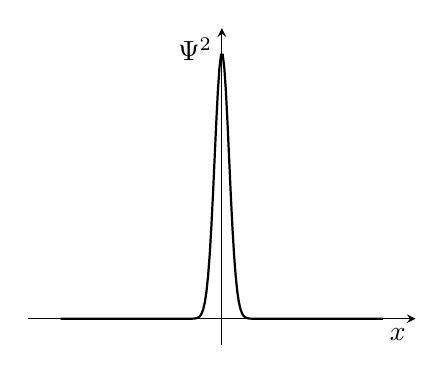
\begin{tikzpicture}
\begin{axis}[small,axis lines=middle,xlabel={$x$},ylabel={$\abs{\Psi}^2$},xtick={\empty},xticklabels={$C$},ytick={\empty},ylabel style={at={(current axis.above origin)},anchor=north east},xlabel style={at={(current axis.right of origin)},anchor=north east},enlargelimits]
\addplot [thick,domain=-0.5:0.5,samples=200,]	{exp(-1000*(x-0)^2)};
\end{axis}
\end{tikzpicture}
\caption{ڈیراک ڈیلٹا تفاعل (مساوات \حوالہ{مساوات_شروڈنگر_ڈیلٹا_تفاعل_تعریف})}
\label{شکل_غیر_تابع_ڈیراک_ڈیلٹا_تفاعل}
\end{figure}

نقطہ \عددی{x=0} پر یہ تفاعل متناہی نہیں ہے لہٰذا تکنیکی طور پر اس کو تفاعل کہنا غلط ہو گا (ریاضی دان اسے \اصطلاح{\footnotesize{متعمم تفاعل}}\فرہنگ{متعمم!تفاعل}\حاشیہب{generalized function}\فرہنگ{generalized!function} یا \اصطلاح{\footnotesize{متعمم تقسیم}}\فرہنگ{متعمم!تقسیم}\حاشیہب{generalized distribution}\فرہنگ{generalized!distribution} کہتے ہیں)۔\حاشیہد{ڈیلٹا تفاعل کو ایسے مستطیل (یا مثلث) کی تحدیدی صورت تصور کیا جا سکتا ہے جس کی چوڑائی بتدریج کم اور قد بتدریج بڑھتا ہو۔} تاہم اس کا تصور نظریہ طبیعیات میں اہم کردار ادا کرتا ہے۔ (مثال کے طور پر، برقی حرکیات کے میدان میں نقطی بار کی کثافت بار ایک ڈیلٹا تفاعل ہو گا۔) آپ دیکھ سکتے ہیں کہ \عددی{\delta(x-a)} نقطہ \عددی{a} پر اکائی رقبہ کا نوکیلی تفاعل ہو گا۔ چونکہ \عددی{\delta(x-a)} اور ایک سادہ تفاعل \عددی{f(x)} کا حاصل ضرب نقطہ \عددی{a} کے علاوہ ہر مقام پر صفر ہو گا لہٰذا \عددی{\delta(x-a)} کو \عددی{f(x)} سے ضرب دینا، اسے \عددی{f(a)} سے ضرب دینے کے مترادف ہے:
\begin{align}
f(x)\delta(x-a)=f(a)\delta(x-a)
\end{align}
بالخصوص درج ذیل لکھا جا سکتا ہے جو ڈیلٹا تفاعل کی اہم ترین خاصیت ہے۔ 
\begin{align}\label{مساوات_شروڈنگر_ڈیلٹا_تفاعل_اٹھاتا_ہے}
\int_{-\infty}^{+\infty}f(x)\delta(x-a)\dif{x}=f(a)\int_{-\infty}^{+\infty}\delta(x-a)\dif{x}=f(a)
\end{align}
 تکمل کی علامت کے اندر یہ نقطہ \عددی{a} پر تفاعل \عددی{f(x)} کی قیمت "اٹھاتا" ہے۔ (لازمی نہیں کہ تکمل \عددی{-\infty} تا \عددی{+\infty} ہو، صرف اتنا ضروری ہے کہ تکمل کے دائرہ کار میں نقطہ \عددی{a} شامل ہو لہٰذا \عددی{a-\epsilon} تا \عددی{a+\epsilon} تکمل لینا کافی ہو گا جہاں \عددی{\epsilon>0} ہے۔) 

آئیں درج ذیل روپ کے مخفیہ پر غور کریں جہاں \عددی{\alpha} ایک مثبت مستقل ہے۔\حاشیہد{ڈیلٹا تفاعل کی اکائی ایک بٹا لمبائی ہے (مساوات \حوالہ{مساوات_شروڈنگر_ڈیلٹا_تفاعل_تعریف} دیکھیں) لہٰذا \عددی{\alpha} کا بُعد توانائی ضرب لمبائی ہو گا۔}
\begin{align}\label{مساوات_شروڈنگر_کنواں_مخفیہ}
V(x)=-\alpha\delta(x)
\end{align}
یہ جان لینا ضروری ہے کہ (لامتناہی چوکور کنویں  کی مخفیہ کی طرح) یہ ایک مصنوعی مخفیہ ہے، تاہم اس کے ساتھ کام کرنا نہایت آسان ہے، اور جو کم سے کم تحلیلی پریشانیاں پیدا کیے بغیر، بنیادی نظریہ پر روشنی ڈالنے میں مددگار ثابت ہوتا ہے۔ ڈیلٹا تفاعل کنویں  کے لیے شروڈنگر مساوات درج ذیل روپ اختیار کرتی ہے
\begin{align}
-\frac{\hslash^{2}}{2m}\frac{\dif^{\,2}\psi}{\dif{x^{2}}}-\alpha\delta(x)\psi=E\psi
\end{align} 
جو مقید حالات \عددی{(E< 0)} اور بکھراو حالات \عددی{(E> 0)} دونوں پیدا کرتی ہے۔

 ہم پہلے مقید حالات پر غور کرتے ہیں۔ خطہ \عددی{x< 0} میں \عددی{V(x)=0} ہو گا لہٰذا 
\begin{align}\label{مساوات_شروڈنگر_ڈیلٹا_تفاعل_الف}
\frac{\dif^{\,2}\psi}{\dif{x^{2}}}=-\frac{2mE}{\hslash^{2}}\psi=k^{2}\psi
\end{align}
لکھا جا سکتا ہے جہاں \عددی{k} درج ذیل ہے (مقید حال کے لئے \عددی{E} منفی ہو گا لہٰذا \عددی{k} حقیقی اور مثبت ہے۔)
\begin{align}\label{مساوات_شروڈنگر_تعریف_کے}
k\equiv\frac{\sqrt{-2mE}}{\hslash}
\end{align}
 مساوات \حوالہ{مساوات_شروڈنگر_ڈیلٹا_تفاعل_الف} کا عمومی حل 
\begin{align}
\psi(x)=Ae^{-kx}+Be^{kx}
\end{align}
ہو گا جہاں \عددی{x\to-\infty} پر پہلا جزو لا متناہی کی طرف بڑھتا ہے لہٰذا ہمیں \عددی{A=0} منتخب کرنا ہو گا: 
\begin{align}\label{مساوات_غیر_تابع_مستقل_بی_والا_جزو}
\psi(x)&=Be^{kx},&& (x<0)
\end{align}
خطہ \عددی{x>0} میں بھی \عددی{V(x)} صفر ہے اور عمومی حل \عددی{F e^{-kx}+G e^{kx}} ہو گا؛ اب \عددی{x\to +\infty} پر دوسرا جزو لامتناہی کی طرف بڑھتا ہے لہٰذا \عددی{G=0} منتخب کرتے ہوئے درج ذیل لیا جائے گا۔
\begin{align}
\psi(x)&=Fe^{-kx},&& (x>0)
\end{align}
 ہمیں نقطہ \عددی{x=0} پر سرحدی شرائط استعمال کرتے ہوئے ان دونوں تفاعل کو ایک  ساتھ جوڑنا ہو گا۔ میں  \عددی{\psi} کے معیاری سرحدی شرائط پہلے بیان کر چکا ہوں
\begin{align}
\begin{cases}
1. \quad\psi & \text{\RL{لازماً استمراری}}\\
2. \quad \frac{\dif{\psi}}{\dif{x}} & \text{\RL{استمراری، ماسوائے ان نقاط پر جہاں مخفیہ لامتناہی ہو}}
\end{cases}
\end{align}
 یہاں اول سرحدی شرط کے تحت \عددی{F=B} ہو گا لہٰذا درج ذیل ہو گا۔ 
\begin{align}\label{مساوات_شروڈنگر-ڈیلٹا_تفاعل_حال}
\psi(x)=
\begin{cases}
Be^{kx},&(x\le0)\\
Be^{-kx},&(x\ge0)
\end{cases}
\end{align} 

تفاعل \عددی{\psi(x)} کو شکل \حوالہ{شکل_غیر_تابع_مقید_حال_تفاعل_موج} میں ترسیم کیا گیا ہے۔ دوم سرحدی شرط ہمیں ایسا کچھ نہیں بتاتی ہے؛ (لا متناہی چوکور کنویں  کی طرح) جوڑ پر مخفیہ لا متناہی ہے اور تفاعل کی ترسیل سے واضح ہے کہ \عددی{x=0} پر اس میں بل پایا جاتا ہے۔ مزید اب تک کی کہانی میں ڈیلٹا تفاعل کا کوئی کردار نہیں پایا گیا۔ ظاہر ہے کہ \عددی{x=0} پر \عددی{\psi} کے تفرق میں عدم استمرار یہی ڈیلٹا تفاعل تعین کرے گا۔ میں یہ عمل آپ کو کر کے دکھاتا ہوں جہاں آپ یہ بھی دیکھ پائیں گے کہ کیوں \عددی{\tfrac{\dif \psi}{\dif x}} عموماً استمراری ہوتا ہے۔ 

\begin{figure}
\centering
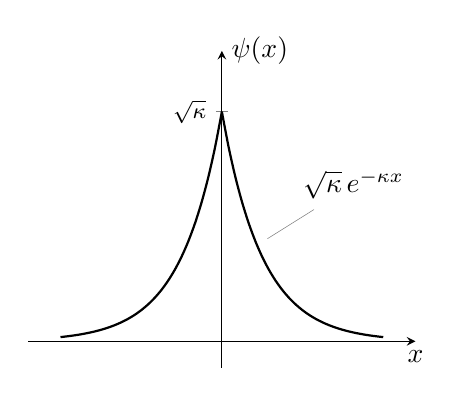
\begin{tikzpicture}[declare function={kpsiA(\x)=e^(\x);kpsiB(\x)=e^(-\x);}]
\begin{axis}[small,axis lines=middle,xlabel={$x$},ylabel={\empty},xlabel style={at={(current axis.right of origin)},anchor={north}},enlargelimits,ytick={1},yticklabels={$\sqrt{\kappa}$}, ylabel={$\psi(x)$},ylabel style={at={(current axis.above origin)},anchor=west},xtick={\empty},ymin=0,ymax=1.15]
\addplot[thick,domain=0:4,smooth] {kpsiB(x)}node[pos=0.25,pin=45:{$\sqrt{\kappa}\,e^{-\kappa x}$}]{};
\addplot[thick,domain=0:-4,smooth] {kpsiA(x)};
\end{axis}
\end{tikzpicture}
\caption{ڈیلٹا تفاعل مخفیہ (مساوات \حوالہ{مساوات_شروڈنگر-ڈیلٹا_تفاعل_حال}) کے لئے مقید حال تفاعل موج۔}
\label{شکل_غیر_تابع_مقید_حال_تفاعل_موج}
\end{figure}

\begin{align}
-\frac{\hslash^2}{2m}\int_{-\epsilon}^{+\epsilon}\frac{\dif^{\,2}\psi}{\dif x^2}\dif x+\int_{-\epsilon}^{+\epsilon}V(x)\psi(x)\dif x=E\int_{-\epsilon}^{+\epsilon}\psi(x)\dif x
\end{align}
پہلا تکمل درحقیقت دونوں آخری نقاط پر \عددی{\tfrac{\dif\psi}{\dif x}} کی قیمتیں ہوں گی؛ آخری تکمل اس پٹی کا رقبہ ہو گا، جس کا قد متناہی، اور \عددی{\epsilon\to 0} کی تحدیدی صورت میں، چوڑائی صفر کو پہنچتی ہو، لہٰذا یہ تکمل صفر ہو گا۔ یوں درج ذیل ہو گا۔
\begin{align}
\Delta\Big(\frac{\dif\psi}{\dif x}\Big)\equiv \left.\frac{\partial \psi}{\partial x}\right|_{+\epsilon}-\left.\frac{\partial \psi}{\partial x}\right|_{-\epsilon}=\frac{2m}{\hslash^2}\lim_{\epsilon\to0}\int_{-\epsilon}^{+\epsilon}V(x)\psi(x)\dif x
\end{align}
 عمومی طور پر دائیں ہاتھ پر حد صفر کے برابر ہو گا لہٰذا \عددی{\tfrac{\dif\psi}{\dif x}} عموماً استمراری ہو گا۔ لیکن جب سرحد پر \عددی{V(x)} لامتناہی ہو تب یہ دلیل قابل قبول نہیں ہو گی۔ بالخصوص \عددی{V(x)=-\alpha\delta(x)} کی صورت میں مساوات \حوالہ{مساوات_شروڈنگر_ڈیلٹا_تفاعل_اٹھاتا_ہے} درج ذیل دے گی: 
\begin{align}\label{مساوات_شروڈنگر_مبدا_پر_تفرقات_کا_فرق}
\Delta\Big(\frac{\dif \psi}{\dif x}\Big)=-\frac{2m\alpha}{\hslash^2}\psi(0)
\end{align}
یہاں درج ذیل ہو گا (مساوات \حوالہ{مساوات_شروڈنگر-ڈیلٹا_تفاعل_حال}):
\begin{align*}
\begin{cases}
\frac{\dif \psi}{\dif x}=-Bke^{-kx},&(x>0)\quad \implies \left.\frac{\dif\psi}{\dif x}\right|_{+}=-Bk\\
\frac{\dif \psi}{\dif x}=+Bke^{+kx},&(x<0)\quad \implies \left.\frac{\dif\psi}{\dif x}\right|_{-}=+Bk
\end{cases}
\end{align*}
لہٰذا \عددی{\Delta(\dif\psi/\dif x)=-2Bk} ہو گا۔ساتھ ہی \عددی{\psi(0)=B} ہے۔ اس طرح مساوات \حوالہ{مساوات_شروڈنگر_مبدا_پر_تفرقات_کا_فرق} درج ذیل کہتی ہے:
\begin{align}
k=\frac{m\alpha}{\hslash^2 }
\end{align}
اور اجازتی توانائیاں درج ذیل ہوں گی (مساوات \حوالہ{مساوات_شروڈنگر_تعریف_کے})۔
\begin{align}
E=-\frac{\hslash^2 k^2}{2m}=-\frac{m\alpha^2}{2\hslash^2}
\end{align}
 آخر میں \عددی{\psi} کو معمول پر لاتے ہوئے 
\begin{align*}
\int_{-\infty}^{+\infty}\abs{\psi(x)}^2\dif x=2\abs{B}^2\int_0^{\infty}e^{-2kx}\dif x=\frac{\abs{B}^2}{k}=1
\end{align*}
 (اپنی آسانی کے لیے مثبت حقیقی جذر کا انتخاب کر کے) درج ذیل حاصل ہو گا۔
\begin{align}
B=\sqrt{k}=\frac{\sqrt{m\alpha}}{\hslash}
\end{align}
آپ دیکھ سکتے ہیں کہ ڈیلٹا تفاعل،کی "زور" \عددی{\alpha} کے قطع نظر، ٹھیک ایک مقید حال دیتا ہے۔ 
\begin{align}\label{مساوات_شروڈنگر_مقید_حال_ڈیلٹا}
\psi(x)&=\frac{\sqrt{m\alpha}}{\hslash}e^{-m\alpha\abs{x}/\hslash^2};&&E=-\frac{m\alpha^2}{2\hslash^2}
\end{align}

ہم \عددی{E>0} کی صورت میں \ترچھا{بکھراو حالات} کے بارے میں کیا کہہ سکتے ہیں؟ شروڈنگر مساوات \عددی{x<0} کے لئے درج ذیل روپ اختیار کرتی ہے
\begin{align*}
\frac{\dif^{\,2}\psi}{\dif x^2}=-\frac{2mE}{\hslash^2}\psi=-k^2\psi
\end{align*}
 جہاں
\begin{align}\label{مساوات_شروڈنگر_مستقل_کے}
k\equiv\frac{\sqrt{2mE}}{\hslash}
\end{align}
 حقیقی اور مثبت ہے۔ اس کا عمومی حل درج ذیل ہے
\begin{align}\label{مساوات_شروڈنگر_بایاں_حل_ڈیلٹا}
\psi(x)=Ae^{ikx}+Be^{-ikx}
\end{align}
جہاں کوئی بھی جزو بے قابو نہیں بڑھتا ہے لہٰذا انہیں رد نہیں کیا جا سکتا ہے۔ اسی طرح \عددی{x>0} کے لئے درج ذیل ہو گا۔
\begin{align}\label{مساوات_شروڈنگر_دایاں_حل_ڈیلٹا}
\psi(x)=Fe^{ikx}+Ge^{-ikx}
\end{align}
نقطہ \عددی{x=0} پر \عددی{\psi(x)} کے استمرار کی بنا پر درج ذیل ہو گا۔
\begin{align}\label{مساوات_شروڈنگر_شرط_اول}
F+G=A+B
\end{align}
تفرقات درج ذیل ہوں گے۔
\begin{align*}
\begin{cases}
\frac{\dif\psi}{\dif x}=ik(Fe^{ikx}-Ge^{-ikx}),& (x>0),\implies \left.\frac{\dif\psi}{\dif x}\right|_{+}=ik(F-G)\\
\frac{\dif\psi}{\dif x}=ik(Ae^{ikx}-Be^{-ikx}),& (x<0),\implies \left.\frac{\dif\psi}{\dif x}\right|_{-}=ik(A-B)
\end{cases}
\end{align*}
لہٰذا \عددی{\Delta(\dif\psi/\dif x)=ik(F-G-A+B)} ہو گا۔ساتھ ہی \عددی{\psi(0)=(A+B)} ہو گا لہٰذا دوسری سرحدی شرط (مساوات \حوالہ{مساوات_شروڈنگر_مبدا_پر_تفرقات_کا_فرق}) کہتی ہے
\begin{align}
ik(F-G-A+B)=-\frac{2m\alpha}{\hslash^2}(A+B)
\end{align}
یا مختصراً:
\begin{align}\label{مساوات_شروڈنگر_شرط_دوم}
F-G&=A(1+2i\beta)-B(1-2i\beta),&&\beta\equiv\frac{m\alpha}{\hslash^2 k}
\end{align}
دونوں سرحدی شرائط مسلط کرنے کے بعد ہمارے پاس دو مساوات (مساوات \حوالہ{مساوات_شروڈنگر_شرط_اول} اور \حوالہ{مساوات_شروڈنگر_شرط_دوم}) جبکہ چار نا معلوم مستقلات \عددی{A}، \عددی{B}، \عددی{C} اور \عددی{D} بلکہ \عددی{k} شامل کرتے ہوئے پانچ نا معلوم مستقل ہوں گے۔ یہ معمول پر لانے کے قابل حال نہیں ہے لہٰذا معمول پر لانا مدد گار ثابت نہیں ہو گا۔ بہتر ہو گا کہ ہم رک کر ان مستقلات کی انفرادی طبیعی اہمیت پر غور کریں۔ آپ کو یاد ہو گا کہ \عددی{e^{ikx}} (کے ساتھ تابع وقت جزو ضربی \عددی{e^{-iEt/\hslash}} منسلک کرنے سے) دائیں رخ حرکت کرتا ہوا تفاعل موج پیدا ہوتا ہے۔ اسی طرح \عددی{e^{-ikx}} بائیں رخ حرکت کرتا ہوا موج دیتا ہے۔ یوں مساوات \حوالہ{مساوات_شروڈنگر_بایاں_حل_ڈیلٹا} میں مستقل \عددی{A} بائیں سے آمدی موج کا حیطہ ہے، \عددی{B} بائیں رخ واپس لوٹتے ہوئے موج کا حیطہ ہے، \عددی{F} (مساوات \حوالہ{مساوات_شروڈنگر_دایاں_حل_ڈیلٹا}) دائیں رخ نکل کر چلتے ہوئے موج کا حیطہ جبکہ \عددی{H} دائیں سے آمدی موج کا حیطہ ہے (شکل \حوالہ{شکل_غیر_تابع_ڈیلٹا_کنواں_سے_بکھراو} دیکھیں)۔ بکھراو کے عمومی تجربہ میں عموماً ایک رخ (مثلاً بائیں) سے ذرات پھینکے جاتے ہیں۔ ایسی صورت میں دائیں جانب سے آمدی موج کا حیطہ صفر ہو گا:
\begin{align}
G&=0,\quad\text{\RL{بائیں سے بکھراو}}
\end{align}

\begin{figure}
\centering
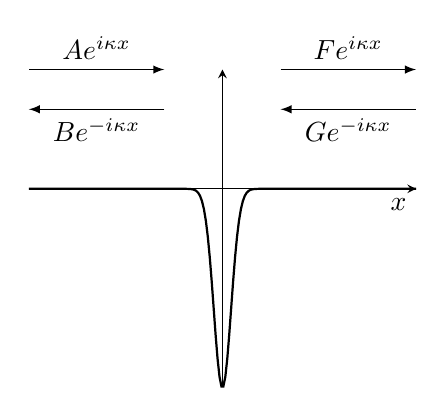
\begin{tikzpicture}
\begin{axis}[clip=false,small,axis lines=middle,xlabel={$x$},ylabel={\empty},xtick={\empty},ytick={\empty},ylabel style={at={(current axis.above origin)},anchor=north east},xlabel style={at={(current axis.right of origin)},anchor=north east}]
\addplot [thick,domain=-0.5:0.5,samples=200,]	{-exp(-1000*(x-0)^2)};
\addplot[-latex] coordinates {(-0.15,0.4)(-0.5,0.4)}node[pos=0.5,below]{$Be^{-i\kappa x}$};
\addplot[latex-] coordinates {(-0.15,0.6)(-0.5,0.6)}node[pos=0.5,above]{$Ae^{i\kappa x}$};
\addplot[latex-] coordinates {(0.15,0.4)(0.5,0.4)}node[pos=0.5,below]{$Ge^{-i\kappa x}$};
\addplot[-latex] coordinates {(0.15,0.6)(0.5,0.6)}node[pos=0.5,above]{$Fe^{i\kappa x}$};
\end{axis}
\end{tikzpicture}
\caption{ڈیلٹا تفاعل کنویں  سے بکھراو۔}
\label{شکل_غیر_تابع_ڈیلٹا_کنواں_سے_بکھراو}
\end{figure}
\اصطلاح{آمدی موج}\فرہنگ{موج!آمدی}\حاشیہب{incident wave}\فرہنگ{wave!incident} کا حیطہ \عددی{A}، \اصطلاح{منعکس موج}\فرہنگ{موج!منعکس}\حاشیہب{reflected wave}\فرہنگ{wave!reflected} کا حیطہ \عددی{B} جبکہ \اصطلاح{ترسیلی موج}\فرہنگ{موج!ترسیلی}\حاشیہب{transmitted wave}\فرہنگ{wave!transmitted} کا حیطہ \عددی{F} ہو گا۔ مساوات \حوالہ{مساوات_شروڈنگر_شرط_اول} اور \حوالہ{مساوات_شروڈنگر_شرط_دوم} کو \عددی{B} اور \عددی{F} کے لیے حل کر کے درج ذیل حاصل ہوں گے۔
\begin{align}
B=\frac{i\beta}{1-i\beta}A,\quad F=\frac{1}{1-i\beta}A
\end{align}
(اگر آپ دائیں سے بکھراو کا مطالعہ کرنا چاہیں تب \عددی{A=0} ہو گا؛ \عددی{G} آمدی حیطہ، \عددی{F} منعکس حیطہ، اور \عددی{B} ترسیلی حیطہ ہوں گے۔)

چونکہ کسی مخصوص مقام پر ذرے کی موجودگی کا احتمال \عددی{\abs{\psi}} ہوتا ہے لہٰذا آمدی ذرہ کے انعکاس کا \ترچھا{تناسبی}\حاشیہد{یہ معمول پر لانے کے قابل تفاعل نہیں ہے لہٰذا کسی ایک مخصوص نقطہ پر ذرہ پایا جانے کا احتمال بے معنی ہو گا؛ بہر حال آمدی اور منعکس امواج کے احتمالات کا تناسب معنی خیز ہے۔ اگلے پیراگراف میں اس پر مزید بات کی جائے گی۔} احتمال درج ذیل ہو گا

\begin{align}
R=\frac{\abs B^{2}}{\abs A^{2}}=\frac{\beta^{2}}{1+\beta^{2}}
\end{align}
جہاں \عددی{ R}کو\اصطلاح{ شرح انعکاس}\فرہنگ{انعکاس!شرح}\حاشیہب{reflection coefficient}\فرہنگ{reflection!coefficient} کہتے ہیں۔ (اگر آپ کے پاس ذرات کی ایک شعاع ہو تو \عددی{R} آپ کو بتائے گا کہ ٹکرانے کے بعد ان میں سے کتنے ذرات واپس لوٹ کر آئیں گے۔) ترسیل کا احتمال درج ذیل ہو گا جسے\اصطلاح{ شرح ترسیل}\فرہنگ{ترسیل!شرح}\حاشیہب{transmission coefficient}\فرہنگ{transmission!coefficient} کہتے ہیں۔
\begin{align}
T=\frac{\abs F^{2}}{\abs A^{2}}=\frac{1}{1+\beta^{2}}
\end{align}
 ظاہر ہے ان احتمال کا مجموعہ ایک \عددی{ (1)} ہو گا۔
 \begin{align}
 R+T=1
 \end{align}
 دھیان رہے کہ \عددی{ R } اور \عددی{ T } متغیر \عددی{ \beta } کے اور لہٰذا (مساوات \حوالہ{مساوات_شروڈنگر_مستقل_کے} اور \حوالہ{مساوات_شروڈنگر_شرط_دوم}) \عددی{ E } کے تفاعل ہوں گے۔
 \begin{align}\label{مساوات_شروڈنگر_انعکاس_ترسیل_مستقل}
 R&=\frac{1}{1+\tfrac{2\hslash^{2}E}{m\alpha^{2}}},&& T =\frac{1}{1+\tfrac{m\alpha^{2}}{2\hslash^{2}E}}
 \end{align} 
توانائی جتنی زیادہ ہو ، ترسیل کا احتمال اتنا ہی زیادہ ہو گا ( جیسا کہ ظاہری طور پر ہونا چاہیے)۔ 
 
 یہاں تک باقی سب ٹھیک ہے تاہم ایک اصولی مسئلہ باقی ہے جسے ہم نظرانداز نہیں کر سکتے ہیں۔ چونکہ بکھراو موج کے تفاعل معمول پر لانے کے قابل نہیں ہیں لہٰذا یہ کسی صورت بھی حقیقی ذرے کے حال کو ظاہر نہیں کر سکتے ہیں۔ تاہم ہم اس مسئلے کا حل جانتے ہیں۔ جیسا ہم نے آزاد ذرہ کے لیے کیا تھا، ہمیں ساکن حالات کے ایسے خطی جوڑ تیار کرنے ہونگے جو معمول پر لائے جانے کے قابل ہوں۔ حقیقی طبی ذرات کو یوں تیار کردہ موجی اکٹھ ظاہر کرے گا۔ یہ ظاہری طور پر سیدھا سادہ اصول ہے جو عملی استعمال میں پیچیدہ ثابت ہوتا ہے لہٰذا یہاں سے آگے مسئلے کو کمپیوٹر کی مدد سے حل کرنا بہتر ہو گا۔\حاشیہد{کنواں اور رکاوٹوں سے موجی اکٹھ کے بکھراو کے اعدادی مطالعہ دلچسپ معلومات فراہم کرتے ہیں۔} چونکہ توانائی کی قیمتوں کا پورا سلسلہ استعمال کیے بغیر آزاد ذرے کے تفاعل موج کو معمول پر نہیں لایا جا سکتا ہے لہٰذا \عددی{ R } اور \عددی{ T } کو (بالترتیب) \عددی{ E } کے قریب ذرات کی تخمینی شرح انعکاس اور شرح ترسیل سمجھنا چاہیے۔ 
 
 یہ ایک عجیب بات ہے کہ ہم لب لباب وقت کے تابع مسئلہ (جہاں ایک آمدی ذرہ مخفیہ سے بکھر کر لامتناہی کی طرف رواں ہوتا ہے) پر غور،  \ترچھا{ ساکن حالات} استعمال کرتے ہوئے کر پاتے ہیں۔ آخر کار (مساوات \حوالہ{مساوات_شروڈنگر_بایاں_حل_ڈیلٹا} اور \حوالہ{مساوات_شروڈنگر_دایاں_حل_ڈیلٹا} میں) \عددی{ \psi }ایک مخلوط، غیر تابع وقت، سائن نما تفاعل ہے جو (مستقل حیطہ کے ساتھ) دونوں اطراف لا متناہی تک پھیلا ہوا ہے۔ اس کے باوجود اس تفاعل پر موزوں سرحدی شرائط مسلط کر کے ہم ایک ذرہ (جسے مقامی موجی اکٹھ سے ظاہر کیا گیا ہو) کی مخفیہ سے انعکاس یا ترسیل کا احتمال تعین کر پاتے ہیں۔ اس ریاضیاتی کرامت کی وجہ میرے خیال میں یہ حقیقت ہے کہ ہم پوری فضا میں پھیلے ہوئے، حقیقتاً حقیر تابعیت وقت کے  تفاعل موج کے خطی جوڑ لے کر ایک (حرکت پذیر) نقطہ کے گرد ایسا تفاعل موج تیار کر سکتے ہیں جس پر وقت کے لحاظ سے تفصیلًا غور کیا جا سکتا ہے(سوال \حوالہ{سوال_شروڈنگر_ساکن_گاوسی_آزاد_ذرہ_موجی_اکٹھ})
 
 \begin{figure}
\centering
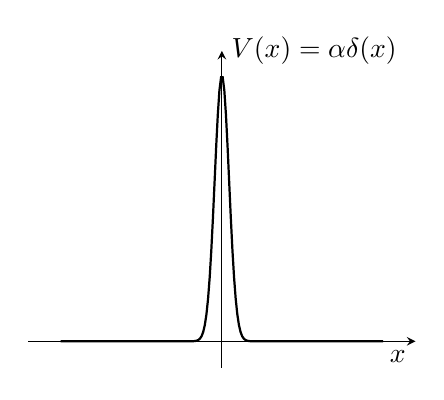
\begin{tikzpicture}
\begin{axis}[clip=false,small,axis lines=middle,xlabel={$x$},ylabel={$V(x)=\alpha\delta(x)$},xtick={\empty},ytick={\empty},ylabel style={at={(current axis.above origin)},anchor=west},xlabel style={at={(current axis.right of origin)},anchor=north east},enlargelimits]
\addplot [thick,domain=-0.5:0.5,samples=200,]	{exp(-1000*(x-0)^2)};
\end{axis}
\end{tikzpicture}
\caption{ڈیلٹا تفاعل رکاوٹ۔}
\label{شکل_غیر_تابع_ڈیلٹا_تفاعل_رکاوٹ}
\end{figure}
متعلقہ مساوات جانتے ہوئے آئیں ڈیلٹا تفاعل رکاوٹ ( شکل \حوالہ{شکل_غیر_تابع_ڈیلٹا_تفاعل_رکاوٹ}) کے مسئلہ پر غور کریں۔ ہمیں صرف \عددی{ \alpha} کی علامت تبدیل کرنی ہو گی۔ ظاہر ہے یہ تحدیدی حال کو ختم کرے گا (سوال \حوالہ{سوال_شروڈنگر_کم_سے_کم_توانائی})۔ دوسری جانب، شرح انعکاس اور شرح ترسیل جو \عددی{ \alpha^2} پر منحصر ہیں تبدیل نہیں ہوں گے۔ کتنی عجیب بات ہے کہ  ذرہ ایک رکاوٹ کے اندر سے یا ایک کنویں  کے اوپر سے ایک جیسی آسانی کے ساتھ گزرتا ہے۔ کلاسیکی طور پر جیسا کہ آپ جانتے ہیں، ایک ذرہ کبھی بھی لا متناہی قد کے رکاوٹ کو عبور نہیں کر سکتا، چاہے اس کی توانائی کتنی ہی کیوں نہ ہو۔ حقیقتاً کلاسیکی مسائل بکھراو غیر دلچسپ ہوتے ہیں: اگر \عددی{ E> V_{\text{بلندتر}}} ہو تب \عددی{ R =0 } اور \عددی{ T=1 } ہو گا اور ذرہ ہر صورت رکاوٹ عبور کر پائے گا؛ اگر \عددی{ E< V_{\text{بلندتر}}} ہو تب \عددی{ T=0 } اور \عددی{ R =1 } ہو گا اور ذرہ پہاڑی پر وہاں تک چڑھے گا جہاں تک اس میں دم ہو اور اس کے بعد اسی راستے واپس لوٹے گا۔ کوانٹائی بکھراو زیادہ دلچسپ ہوتے ہیں: اگر \عددی{ E< V_{\text{بلندتر}} } ہو تب بھی ایک ذرے کا مخفیہ عبور کرنے کا احتمال غیر صفر ہو گا۔ اس مظہر کو \اصطلاح{سرنگ زنی}\فرہنگ{سرنگ زنی}\حاشیہب{tunneling}\فرہنگ{tunneling} کہتے ہیں جس پر جدید برقیات کا بیشتر حصہ منحصر ہے اور جو خوردبین میں حیرت انگیز ترقی کا سبب بنا ہے۔ اس کے برعکس \عددی { E> V_{\text{بلندتر}}} کی صورت میں بھی ذرے کے انعکاس کا احتمال غیر صفر ہو گا؛ اگرچہ میں آپ کو کبھی بھی مشورہ نہیں دوں گا کہ چھت سے نیچے کودیں اور توقع رکھیں کہ کوانٹم میکانیات آپ کی جان بچا پائے گی ( سوال \حوالہ{سوال_غیر_تابع_اچانک_گہرائی} دیکھیے گا)۔
 
\ابتدا{سوال}
درج ذیل تکملات کی قیمتیں تلاش کریں۔ 
\begin{enumerate}[a.]
\item\(\int_{-3}^{+1}(x^{3}-3x^{2}+2x-1) \delta(x+2) \dif{x}\)
\item\( \int_{0}^{\infty}[\cos(3x)+2] \delta(x-\pi) \dif{x}\)
\item\(\int_{-1}^{+1}e^{(\abs x+3)} \delta (x-2) \dif{x}\)
\end{enumerate}
\انتہا{سوال}
\ابتدا{سوال}\شناخت{سوال_شروڈنگر_تفاعلات_برابر}
 ڈیلٹا تفاعلات زیر علامت تکمل رہتے ہیں اور دو فقرے \عددی{ D_{1}(x) } اور \عددی{ D_{2}(x) }جو ڈیلٹا تفاعل پر مبنی ہیں صرف درج صورت میں  برابر ہوں گے
\begin{align*}
\int_{-\infty}^{+\infty}f(x) D_1(x) \dif x =\int_{-\infty}^{+\infty}f(x) D_2(x) \dif x
\end{align*}
 جہاں \عددی{f(x)} کوئی بھی سادہ تفاعل ہو سکتا ہے ۔
\begin{enumerate}[a.]
\item 
درج ذیل دکھائیں
 \begin{align}\delta(cx)=\frac{1}{\abs{c}}\delta(x)\end{align}
جہاں \عددی{c} ایک حقیقی مستقل ہے۔ (منفی \عددی{c} کی صورت میں بھی تصدیق کریں۔) 
\item 
\اصطلاح{ سیڑھی تفاعل }\فرہنگ{سیڑھی تفاعل}\حاشیہب{step function}\فرہنگ{step function}\عددی{\theta(x)} درج ذیل ہے ۔
\begin{align}\label{مساوات_غیر_تابع_شروڈنگر_تھیٹا_سیڑھی_تفاعل}
\theta(x)=
\begin{cases}
1& x>0\\
0& x<0
\end{cases}
\end{align}
 (اس نایاب صورت میں جہاں اس کی ضرورت پیش آتی ہو ، ہم \عددی{\theta(0)} کی تعریف \عددی{\frac{1}{2}} کرتے ہیں۔) دکھائیں کہ \(\dif{\theta}/\dif{x}=\delta(x)\) ہو گا۔
\end{enumerate}
\انتہا{سوال}
\ابتدا{سوال}
 عدم یقینیت کے اصول کو \حوالہ{مساوات_شروڈنگر_مقید_حال_ڈیلٹا}کے تفاعل موج کے لئے پرکھیں۔ \ترچھا{ اشارہ} چونکہ \عددی{ \psi } کے تفرق کا\عددی{x=0} پر عدم استمرار پایا جاتا ہے لہٰذا\عددی{\langle p^2\rangle} کا حساب پیچیدہ ہو گا۔  سوال \حوالہ{سوال_شروڈنگر_تفاعلات_برابر}-ب کا نتیجہ استعمال کریں۔ \ترچھا{جزوی جواب:} \عددی{\langle p^{2}\rangle =(m\alpha/\hslash)^{2}} 
\انتہا{سوال}
\ابتدا{سوال}\شناخت{سوال_شروڈنگر_ڈیلٹا_فوریئر_تبادل_کیا_ہے}
 تفاعل \عددی{\delta(x)} کا فوریئر تبادل کیا ہو گا؟ مسئلہ پلانشرل استعمال کر کے درج ذیل دکھائیں۔ 
\begin{align}\label{مساوات_شروڈنگر_ڈیلٹا_پلانشرال}
\delta(x)=\frac{1}{2\pi}\int_{-\infty}^{+\infty} e^{ikx} \dif{k}
\end{align}
 \ترچھا{تبصرہ:} اس کلیہ دیکھ کر ایک عزت مند ریاضی دان پریشان ضرور ہو گا۔ اگرچہ \عددی{x=0} کے لئے یہ تکمل لامتناہی ہے اور \عددی{x\neq 0} کی صورت میں چونکہ متکمل ہمیشہ کے لئے ارتعاش پذیر رہتا ہے لہٰذا یہ (صفر یا کسی دوسرے عدد کو) مرکوز نہیں ہوتا ہے ۔ اس کی پیوندکاری کے طریقے پائے جاتے ہیں (مثلاً، ہم \عددی{-L} تا \عددی{+L} تکمل لے کر،  مساوات \حوالہ{مساوات_شروڈنگر_ڈیلٹا_پلانشرال} کو، \عددی{L\to\infty} کرتے ہوئے متناہی تکمل کی اوسط قیمت تصور کر سکتے ہیں)۔ یہاں دشواری کا سبب یہ ہے کہ مسئلہ پلانشرل کے (مربع متکاملیت) کی بنیادی شرط کو ڈیلٹا تفاعل مطمئن نہیں کرتا ہے(صفحہ \حوالہصفحہ{حاشیہ_شروڈنگر_مربع_تکملیت} پر مربع متکاملیت کی شرط حاشیہ میں پیش کی گئی ہے)۔ اس کے باوجود مساوات \حوالہ{مساوات_شروڈنگر_ڈیلٹا_پلانشرال} نہایت مددگار ثابت ہو سکتا ہے اگر اس کو احتیاط سے استعمال کیا جائے۔
\انتہا{سوال} 
\ابتدا{سوال}\شناخت{سوال_شروڈنگر_جڑواں_ڈیلٹا}
درج ذیل جڑواں ڈیلٹا تفاعل مخفیہ پر غور کریں جہاں\عددی{ \alpha } اور \عددی{ a} مثبت مستقل ہیں۔
\begin{align*}
V(x)=-\alpha[\delta(x+a)+\delta(x-a)]
\end{align*}
\begin{enumerate}[a.]
\item
 اس مخفیہ کا خاکہ کھینچیں۔
\item
 یہ کتنی مقید حالات پیدا کرتا ہے؟ \عددی{\alpha=\hslash^2/ma } اور \عددی{\alpha=\hslash^2/4ma }کیلئے اجازتی توانائیاں تلاش کریں اور تفاعلات موج کا خاکہ کھینچیں۔
\end{enumerate}
 \انتہا{سوال}
\ابتدا{سوال}
جڑواں ڈیلٹا تفاعل کے مخفیہ ( سوال\حوالہ{سوال_شروڈنگر_جڑواں_ڈیلٹا}) کے لئے شرح ترسیل تلاش کریں۔ 
 \انتہا{سوال}

\حصہ{متناہی چوکور کنواں}
 ہم آخری مثال کے طور پر متناہی چوکور کنویں  کا مخفیہ
\begin{align}\label{مساوات_شروڈنگر_متناہی_چکور_کنواں_مخفیہ}
V(x)=
 \begin{cases} 
  -V_{0} & -a< x< a \\
  0 & \abs{x}> a
 \end{cases}
\end{align}
لیتے ہیں جہاں\عددی{ V_{0} } ایک( مثبت) مستقل ہے (شکل  \حوالہ{شکل_غیر_تابع_متناہی_کنواں})۔ ڈیلٹا تفاعل کنویں  کی طرح یہ مخفیہ مقید حالات ( جہاں\عددی{ E< 0 } ہو گا ) کے ساتھ ساتھ بکھراو حالات ( جہاں\عددی{ E> 0 } ہو گا) بھی پیدا کرتا ہے۔ ہم پہلے مقید حالات پر غور کرتے ہیں۔
 
 %fig 2.17 pg 90
\begin{figure}
\centering
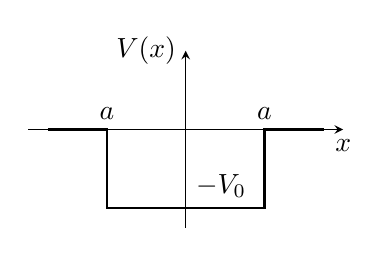
\begin{tikzpicture}
%\draw[help lines, thick,gray,step=1] (0,0) grid (12,12);
\draw[-stealth] (-2,0) -- (2,0) node[below]{$x$};
\draw[-stealth] (0,-1.25) -- (0,1) node[left]{$V(x)$};
\draw[thick] (-1.75,0) -- (-1,0) node[above]{$a$} --++ (0,-1) --++ (2,0) node[pos=0.5, above right]{$-V_{0}$} --++ (0,1) node[above]{$a$} --++ (0.75,0);
\end{tikzpicture}
\caption{متناہی چوکور کنواں (مساوات \حوالہ{مساوات_شروڈنگر_متناہی_چکور_کنواں_مخفیہ})۔}
\label{شکل_غیر_تابع_متناہی_کنواں}
\end{figure}
 
 خطہ\عددی{ x< -a } میں جہاں مخفیہ صفر ہے، شروڈنگر مساوات درج ذیل روپ اختیار کرتی ہے
\begin{align*}
\frac{\dif^{\,2}\psi}{\dif{x^{2}}}=\kappa^{2}\psi \quad \text{یا}\quad -\frac{\hslash^{2}}{2m} \frac{\dif^{\,2} \psi}{\dif{x^{2}}}=E\psi
\end{align*} 
جہاں
 \begin{align}\label{مساوات_شروڈنگر_مستقل_کپا}
 \kappa\equiv \frac{\sqrt{-2mE}}{\hslash}
 \end{align}
 حقیقی اور مثبت ہے۔ اس کا عمومی حل\عددی{\Psi(x)=A e^{-kx}+ B e^{kx} } ہے لیکن   \عددی{ x\to -\infty } کے صورت میں اس کا پہلا جزو بے قابو بڑھتا ہے لہٰذا ( ہمیشہ طرح؛ مساوات \حوالہ{مساوات_غیر_تابع_مستقل_بی_والا_جزو} دیکھیں) طبی طور پر قابل قبول حل درج ذیل ہو گا۔
\begin{align} 
\psi(x)&=Be^{kx}, && x<-a
\end{align}
 خطہ\عددی{ -a< x < a } میں جہاں \عددی{ V(x)=-V_{0} } ہے شروڈنگر مساوات درج ذیل روپ اختیار کرے گی
\begin{align*}
\frac{\dif ^{\,2}\psi}{\dif{x^2}}=-l^2\psi \quad \text{یا}\quad -\frac{\hslash^2}{2m}\frac{\dif^{\,2}\psi}{\dif x^2}=-V_0\psi
 \end{align*}
 جہاں \عددی{l} درج ذیل ہے۔
 \begin{align}\label{مساوات_شروڈنگر_مستقل_ایل}
 l\equiv \frac{\sqrt{2m(E+V_{0})}}{\hslash} 
 \end{align}
 اگرچہ مقید حالات کے لئے \عددی{ E } منفی ہے تاہم \عددی{E> V_{\text{کمتر}}} کی بنا پر ( سوال \حوالہ{سوال_شروڈنگر_کم_سے_کم_توانائی} دیکھیں)  اس کو \عددی{ -V_{0} } سے بڑا ہونا ہو گا ؛ لہٰذا \عددی{ l} بھی حقیقی اور مثبت ہو گا۔ اس کا عمومی حل درج ذیل ہو گا\حاشیہد{آپ چاہیں تو عمومی حل کو قوت نمائی روپ \عددی{(C'e^{ilx}+D'e^{-ilx})} میں لکھ سکتے ہیں۔اس سے بھی وہی اختتامی نتائج حاصل ہوں گے، تاہم تشاکلی مخفیہ کی بنا پر ہم جانتے ہیں کہ حل جفت یا طاق ہوں گے، اور \عددی{\sin} اور \عددی{\cos} کا استعمال اس حقیقت کو بلا واسطہ بروئے کار لا سکتا ہے۔}
 \begin{align}
 \psi(x)&=C\sin(lx)+D\cos(lx), && -a<x<a
 \end{align}
 جہاں\عددی{ C } اور\عددی{ D } اختیاری مستقلات ہیں۔ آخر میں، خطہ \عددی{x>a} جہاں ایک بار پھر مخفیہ صفر ہے؛ عمومی حل\عددی{ \psi(x)=F e^{-\kappa x}+G e^{\kappa x} } ہو گا تاہم \عددی{ x\to \infty} کی صورت میں دوسرا جزو بے قابو بڑھتا ہے لہٰذا قابل قبول حل درج ذیل ہو گا۔
\begin{align}
 \psi(x)&=F e^{-\kappa x}, && x>a
\end{align}

 اگلے قدم میں ہمیں سرحدی شرائط مسلط کرنے ہوں گے: \عددی{ \psi }اور \عددی{ \frac{\dif{\psi}}{\dif{x}} } نقاط \عددی{ -a } اور\عددی{ +a } پر استمراری ہیں۔ یہ جانتے ہوئے کہ دیا گیا مخفیہ جفت تفاعل ہے، ہم کچھ وقت بچا سکتے ہیں اور فرض کر سکتے ہیں کہ حل مثبت یا طاق ہوں گے ( سوال \حوالہ{سوال_غیر_تابع_پہلا_سوال}-ج)۔ اس کا فائدہ یہ ہے کہ ہمیں صرف ایک جانب ( مثلاً\عددی{ +a } ) پر سرحدی شرائط مسلط کرنی ہوں گی؛ چونکہ\عددی{ \psi(-x)=\pm \psi(x) } ہے لہٰذا دوسری جانب کا حل ہمیں خود بخود حاصل ہو گا۔ میں جفت حل حاصل کرتا ہوں جبکہ آپ کو سوال \حوالہ{سوال_غیر_تابع_متناہی_چکور_طاق_دیکھو} میں طاق حل تلاش کرنے کو کہا گیا ہے۔ \عددی{ \cos}جفت ہے (جبکہ\عددی{ \sin} طاق ہے) لہٰذا میں درج ذیل روپ کے حلوں کی تلاش میں ہوں۔ 
\begin{align}\label{مساوات_شروڈنگر_تلاش_تفاعلات}
\psi(x)=
\begin{cases}
Fe^{-\kappa x} & x> a\\
D\cos(l x) & 0< x < a\\
\psi(-x) & x< 0
\end{cases}
\end{align}
نقطہ\عددی{ x=a } پر \عددی{\psi(x)} کی استمرار درج ذیل کہتی ہے 
\begin{align}\label{مساوات_شروڈنگر_استمرار_مستقل_الف}
 Fe^{-\kappa a}=D\cos(la) 
 \end{align}
 جبکہ \عددی{\frac{\dif{\psi}}{\dif{x}} } کی استمرار درج ذیل کہتی ہے۔
 \begin{align}\label{مساوات_شروڈنگر_استمرار_مستقل_ب}
 -\kappa Fe^{-\kappa a}=-lD\sin(la) 
 \end{align} 
 مساوات \حوالہ{مساوات_شروڈنگر_استمرار_مستقل_ب} کو مساوات \حوالہ{مساوات_شروڈنگر_استمرار_مستقل_الف} سے تقسیم کرتے ہوئے درج ذیل حاصل ہو گا۔

\begin{align}\label{مساوات_شروڈنگر_حل_کپا}
\kappa =l\tan(la) 
 \end{align}
 چونکہ \عددی{ \kappa} اور \عددی{ l } دونوں \عددی{ E } کے تفاعل ہیں لہٰذا اس کلیہ سے اجازتی توانائیاں حاصل کی جا سکتی ہیں۔اجازتی توانائی\عددی{ E } کے لئے حل کرنے سے پہلے ہم درج ذیل بہتر علامتیں متعارف کرتے ہیں۔
\begin{align}
z\equiv l a \quad \text{اور}\quad z_0\equiv\frac{a}{\hslash}\sqrt{2mV_0}
\end{align} 
مساوات \حوالہ{مساوات_شروڈنگر_مستقل_کپا} اور \حوالہ{مساوات_شروڈنگر_مستقل_ایل} کے تحت \عددی{ (\kappa^{2}+l^{2})=2mV_{0}/\hslash^{2} } ہو گا لہٰذا \عددی{ \kappa a=\sqrt{z_{0}^{2}-z^{2}}} ہو گا اور مساوات \حوالہ{مساوات_شروڈنگر_حل_کپا} درج ذیل روپ اختیار کرے گی۔
\begin{align}\label{مساوات_غیر_تابع_شروڈنگر_ترسیمی_حل}
\tan z=\sqrt{(z_{0}/z)^{2}-1} 
\end{align}
 یہ \عددی{ z} (لہٰذا \عددی{ E}) کی ماورائی مساوات ہے جس کا متغیر \عددی{ z_{0}} ہے ( جو کنویں  کی" جسامت" کی ناپ ہے)۔ اس کو اعدادی طریقہ سے کمپیوٹر کے ذریعے حل کیا جا سکتا یا \عددی{ \tan z} اور \عددی{ \sqrt{(z_{0}/z)^{2}-1}} کو ایک ساتھ ترسیم کر کے ان کے نقاط تقاطع لیتے ہوئے حل کیا جا سکتا ہے ( شکل \حوالہ{شکل_غیر_تابع_شروڈنگر_جفت_حالات_ترسیمی})۔ دو تحدیدی صورتیں زیادہ دلچسپی کے حامل ہیں ۔ 
 
 %fig 2.18 pg 92
\begin{figure}
\centering
\pgfmathsetmacro{\za}{8}
\begin{tikzpicture}[declare function = {fa(\x)=sqrt((\za/\x)^2-1); fb(\x)=tan(deg(\x));}]
\begin{axis}[clip=false,axis lines=middle,xlabel={$z$},ylabel={}, xtick={pi/2,pi,3/2*pi,2*pi,2.5*pi},
 xticklabels={$\pi/2$,$\pi$,$3\pi/2$,$2\pi$,$5\pi/2$}, ytick={\empty}, ylabel style={at={(current axis.above origin)},anchor=north},xlabel style={at={(current axis.right of origin)},anchor=north},xmax=3*pi]
\addplot [name path global=aa,thick,smooth,domain=1:8]{fa(x)}node[pos=0.8,pin={[pin distance=1.5cm]30:{$\sqrt{(z_0/z)^2-1}$}}]{}node[pos=1,above]{$z_0$};
\addplot [name path global=b,thick,smooth,domain=0:0.92*pi/2]{fb(x)}node[pos=0.9,pin={30:{$\tan z$}}]{};
\addplot [name path global=c,thick,smooth,domain=pi:pi+0.92*pi/2]{fb(x)}node[pos=0.9,pin={30:{$\tan z$}}]{};
\addplot [name path global=d,thick,smooth,domain=2*pi:2*pi+0.92*pi/2]{fb(x)}node[pos=0.9,pin={30:{$\tan z$}}]{};
\draw[name intersections={of={aa and b}, by ={k1}}] (k1)node[circle,inner sep=1.5pt,fill=black]{};
\draw[name intersections={of={aa and c}, by ={k1}}] (k1)node[circle,inner sep=1.5pt,fill=black]{};
\draw[name intersections={of={aa and d}, by ={k1}}] (k1)node[circle,inner sep=1.5pt,fill=black]{};
\end{axis}
\end{tikzpicture}
\caption{ترسیمی حل برائے مساوات \حوالہ{مساوات_غیر_تابع_شروڈنگر_ترسیمی_حل} جہاں \عددی{z_0=8} لیا گیا ہے (جفت حالات)۔}
\label{شکل_غیر_تابع_شروڈنگر_جفت_حالات_ترسیمی}
\end{figure}
 
\begin{enumerate}[a.]
\item
\موٹا{ چوڑا اور گہرا کنواں۔}\quad
 بہت بڑی \عددی{ z_{0}} کی صورت میں طاق \عددی{n} کے لئے نقاط تقاطع \عددی{ z_{n}=n\pi/2} سے معمولی نیچے ہوں گے؛ یوں درج ذیل ہو گا۔
\begin{align}
E_{n}+V_{0}\cong \frac{n^{2}\pi^{2}\hslash^{2}}{2m(2a)^{2}}
 \end{align}
اب\عددی{E+V_{0}} \ترچھا{ کنویں  کی تہہ سے زیادہ} توانائی کو ظاہر کرتی ہے اور مساوات کا دایاں ہاتھ ہمیں \عددی{2a} چوڑائی کے لامتناہی چوکور کنویں  کی توانائیاں دیتا ہے ( مساوات\حوالہ{مساوات_شروڈنگر_لامتناہی_چکور_کنواں_توانائیاں} دیکھیں) ؛ بلکہ \عددی{ n} یہاں طاق ہے لہٰذا  توانائیوں کی نصف تعداد حاصل ہو گی۔ ( جیسا آپ سوال \حوالہ{سوال_غیر_تابع_متناہی_چکور_طاق_دیکھو} میں دیکھیں گے کل توانائیوں کی باقی نصف تعداد طاق تفاعل موج سے حاصل ہو گی۔) یوں\عددی{ V_{0}\to \infty } کرنے سے متناہی چوکور کنواں سے لامتناہی چوکور کنواں حاصل ہو گا؛ تاہم کسی بھی متناہی \عددی{ V_{0}} کی صورت میں مقید حالات کی تعداد متناہی ہو گی۔ 
\item 
\موٹا{ کم گہرا، کم چوڑا کنواں}\quad 
 جیسے جیسے\عددی{ z_{0}} کی قیمت کم کی جاتی ہے مقید حالات کی تعداد کم ہوتی جاتی ہے حتٰی کہ آخر کار (\عددی{ (z_{0}< \pi/2) } کیلئے جہاں کم ترین طاق حال بھی نہیں پایا جاتا ) صرف ایک مقید حال رہ جائے گا۔ دلچسپ بات یہ ہے، کنواں جتنا بھی "کمزور"  کیوں نہ ہو ، ایک عدد مقید حال ضرور پایا جائے گا۔ 
\end{enumerate}


 اگر آپ \عددی{ \psi } (مساوات \حوالہ{مساوات_شروڈنگر_تلاش_تفاعلات}) کو معمول پر لانے میں دلچسپی رکھتے ہیں( سوال \حوالہ{سوال_غیر_تابع_معمول_سے_ڈی_ایف}) تو ایسا ضرور کریں جبکہ میں اب بکھراو حالات ( \عددی{ E> 0 }) کی طرف بڑھنا چاہوں گا ۔ بائیں ہاتھ جہاں\عددی{ V(x)=0} ہے درج ذیل ہو گا 
\begin{align}
\psi(x)&=Ae^{i k x}+Be^{-i k x} && (x<-a) 
\end{align}
 جہاں ہمیشہ کی طرح درج ذیل ہو گا۔
 \begin{align}
 k\equiv \frac{\sqrt{2mE}}{\hslash} 
 \end{align} 
 کنویں  کے اندر جہاں\عددی{ V(x)=-V_{0}} ہے درج ذیل ہو گا
\begin{align}
\psi(x)&=C\sin(lx)+D\cos(lx)&& (-a<x<a)
 \end{align}
 جہاں پہلے کی طرح درج ذیل ہو گا۔
 \begin{align}
 l\equiv \frac{\sqrt{2m(E+V_{0})}}{\hslash}
 \end{align}
  دائیں جانب، جہاں ہم فرض کرتے ہیں کہ کوئی آمدی موج نہیں پائی جاتی، درج ذیل ہو گا ۔
 \begin{align}
 \psi(x)=Fe^{i k x} 
 \end{align}
 یہاں آمدی حیطہ \عددی{ A}، انعکاسی حیطہ \عددی{ B} اور ترسیلی حیطہ \عددی{ F} ہے۔\حاشیہد{مقید حالات کی صورت میں ہم نے طاق اور جفت تفاعلات تلاش کیے۔ ہم یہاں بھی ایسا کر سکتے ہیں، تاہم مسئلہ بکھراو میں امواج صرف ایک رخ سے آتے ہیں لہٰذا یہ مسئلہ ذاتی طور پر غیر تشاکلی ہے اور سیاق و سباق کے لحاظ سے (حرکت پذیر امواج کے اظہار کے لئے ) قوت نمائی علامت کا استعمال زیادہ موثر ہے۔ } 
 
 یہاں چار سرحدی شرائط پائے جاتے ہیں: نقطہ \عددی{-a} پر \عددی{\psi(x)} کے استمرار کے تحت درج ذیل ہو گا
\begin{align}\label{مساوات_شروڈنگر_اے}
Ae^{-ika}+Be^{ika} = -C\sin(la)+D\cos(la)
 \end{align}
نقطہ\عددی{ -a } پر\عددی{\tfrac{\dif \psi}{\dif x}} کا استمرار درج ذیل دے گا
\begin{align}\label{مساوات_شروڈنگر_اے_بی}
ik[Ae^{-ika}-Be^{ika}] =l[C\cos(la)+D\sin(la)] 
\end{align}

نقطہ \عددی{ +a } پر \عددی{ \psi(x) }کا استمرار درج ذیل دے گا 
\begin{align}\label{مساوات_شروڈنگر_سی}
C\sin (la)+D\cos(la)]=Fe^{ika} 
\end{align}
اور \عددی{ +a } پر\عددی{\frac{\dif{\psi}}{\dif{x}} } کا استمرار درج ذیل دے گا۔
\begin{align}\label{مساوات_شروڈنگر_ڈی}
l[C\cos(la)-D\sin(la)]=ikFe^{ika} 
\end{align}
 ہم ان میں سے دو کو استعمال کرتے ہوئے \عددی{ C } اور \عددی{ D } خارج کر کے باقی دو کو  \عددی{ B }اور \عددی{ F} کے لئے حل کر سکتے ہیں (سوال \حوالہ{سوال_غیر_تابع_ایک_سے_دوسرا_اخذ} دیکھیے گا)۔
\begin{align}
B&=i\frac{\sin(2la)}{2kl}(l^{2}-k^{2})F \label{مساوات_شروڈنگر_بی}\\
F&=\frac{e^{-2ika}A}{\cos(2la)-i\frac{(k^{2}+l^{2})}{2kl}\sin(2la)}\label{مساوات_شروڈنگر_ایف}
\end{align}
 شرح ترسیل\عددی{(T=\abs{F}^2/\abs{A}^2) }کو اصل متغیرات کی صورت میں لکھتے ہوئے درج ذیل حاصل ہو گا۔

\begin{align}\label{مساوات_شروڈنگر_ترسیلی_حل}
T^{-1}=1+\frac{V_{0}^{2}}{4E(E+V_{0})}\sin^{2}\big(\frac{2a}{\hslash}\sqrt{2m(E+V_{0})} \big) 
 \end{align}
 دھیان رہے کہ جہاں بھی سائن کی قیمت صفر ہو، یعنی درج ذیل نقطوں پر جہاں \عددی{n} عدد صحیح ہے 
 \begin{align}
 \frac{2a}{\hslash}\sqrt{2m(E_{n}+V_{0})}=n\pi 
 \end{align}
 وہاں\عددی{T=1} (اور کنواں "مکمل شفاف" ) ہو گا ۔ یوں مکمل ترسیل کے لیے درکار توانائیاں درج ذیل ہوں گی
\begin{align}
E_{n}+V_{0}=\frac{n^{2}\pi^{2}\hslash^{2}}{2m(2a)^{2}} 
\end{align}
 جو عین لامتناہی چوکور کنویں  کی اجازتی توانائیاں ہیں۔ شکل \حوالہ{شکل_غیر_تابع_شروڈنگر_ترسیلی_مستقل_بطور_تفاعل} میں توانائی کے لحاظ سے \عددی{T} ترسیم کیا گیا ہے۔\حاشیہد{اس حیرت کن مظہر کا مشاہدہ تجربہ گاہ میں بطور \اصطلاح{رمزاور و ٹاونسنڈ اثر}\فرہنگ{رمزاور و ٹاونسنڈ اثر}\تحریر{(Ramsauer-Townsend effect)} کیا گیا ہے۔ }
%fig 2.19 pg 94
\begin{figure}
\centering
\pgfmathsetmacro{\v}{2}
\begin{tikzpicture}[declare function = {ga(\x)=(sqrt(\x+\v));gb(\x)=\v^2/(4*\x*(\x+\v));gc(\x)=(sin(deg(10*ga(\x))))^2;fb(\x)=1+gb(\x)*gc(\x);fa(\x)=1/(fb(\x));}]
\begin{axis}[clip=false,axis lines=middle,xlabel={$E$},ylabel={$T$}, xtick={\empty},
 xticklabels={}, ytick={1}, ylabel style={at={(current axis.above origin)},anchor=east},xlabel style={at={(current axis.right of origin)},anchor=north},ymax=1.2]
\addplot [thick,domain=0:6,samples=100]{fa(x)};
\addplot[dashed]plot coordinates {(0,1)(6,1)};
\end{axis}
\end{tikzpicture}
\caption{ترسیلی مستقل بطور توانائی کا تفاعل (مساوات \حوالہ{مساوات_شروڈنگر_ترسیلی_حل})۔}
\label{شکل_غیر_تابع_شروڈنگر_ترسیلی_مستقل_بطور_تفاعل}
\end{figure}

%==============================================================

\ابتدا{سوال} \شناخت{سوال_غیر_تابع_متناہی_چکور_طاق_دیکھو}
متناہی چوکور کنویں  کے طاق مقید حال کے تفاعل موج کا تجزیہ کریں۔ اجازتی توانائیوں کی ماورائی مساوات اخذ کر کے اسے ترسیمی طور پر حل کریں ۔ اس کے دونوں تحدیدی صورتوں پر غور کریں۔ کیا ہر صورت ایک طاق مقید حال پایا جائے گا ؟ 
\انتہا{سوال}
\ابتدا{سوال}\شناخت{سوال_غیر_تابع_معمول_سے_ڈی_ایف}
 مساوات\حوالہ{مساوات_شروڈنگر_تلاش_تفاعلات} میں دیا گیا \عددی{ \psi(x)} معمول پر لا کر مستقل\عددی{ D } اور\عددی{ F } تعین کریں۔
\انتہا{سوال}
\ابتدا{سوال}
ڈیراک ڈیلٹا تفاعل کو ایک ایسی مستطیل کی تحدیدی صورت تصور کیا جا سکتا ہے، جس کا رقبہ اکائی \عددی{(1) } رکھتے ہوئے اس کی چوڑائی صفر تک اور قد لامتناہی تک پہنچائی جائے۔ دکھائیں کہ ڈیلٹا تفاعل کنواں (مساوات\حوالہ{مساوات_شروڈنگر_کنواں_مخفیہ}) لامتناہی گہرا ہونے کے باوجود \عددی{z_{0}\to 0 }کی بنا پر ایک" کمزور" مخفیہ ہے۔ ڈیلٹا تفاعل مخفیہ کو متناہی چوکور کنویں  کی تحدیدی صورت لیتے ہوئے اس کی مقید حال کی توانائی تعین کریں۔ تصدیق کریں کہ آپ کا جواب مساوات\حوالہ{مساوات_شروڈنگر_مقید_حال_ڈیلٹا} کے مطابق ہے۔ دکھائیں کہ موزوں حد کی صورت میں مساوات\حوالہ{مساوات_شروڈنگر_ترسیلی_حل} کی تخفیف مساوات\حوالہ{مساوات_شروڈنگر_انعکاس_ترسیل_مستقل} دے گی ۔
\انتہا{سوال}
\ابتدا{سوال}\شناخت{سوال_غیر_تابع_ایک_سے_دوسرا_اخذ}
مساوات \حوالہ{مساوات_شروڈنگر_بی} اور \حوالہ{مساوات_شروڈنگر_ایف} اخذ کریں۔\ترچھا{ اشارہ:} مساوات \حوالہ{مساوات_شروڈنگر_سی} اور\حوالہ{مساوات_شروڈنگر_ڈی} سے \عددی{ C } اور \عددی{ D } کو \عددی{ F } کی صورت میں حاصل کر کے
\begin{align*}
C&=[\sin(la)+i\frac{k}{l}\cos(la)]e^{ika}F; && D=[\cos(la)-i\frac{k}{l}\sin(la)]e^{ika}F
 \end{align*}
 انہیں واپس مساوات \حوالہ{مساوات_شروڈنگر_اے} اور \حوالہ{مساوات_شروڈنگر_اے_بی} میں پر کریں۔ شرح ترسیل حاصل کر کے مساوات\حوالہ{مساوات_شروڈنگر_مقید_حال_ڈیلٹا} کی تصدیق کریں۔
\انتہا{سوال}
\ابتدا{سوال}
مستطیلی رکاوٹ ( جسے خطہ\عددی{ -a< x< a } میں\عددی{V_(x)=+V_{0}> 0} لینے سے مساوات \حوالہ{مساوات_شروڈنگر_متناہی_چکور_کنواں_مخفیہ} دیتی ہے) کے لئے شرح ترسیل تعین کریں۔ تین صورتوں \عددی{ E< V_{0}} ،
\عددی{ E=V_{0} }اور \عددی{ E> v_{0} } کو علیحدہ علیحدہ حل کریں۔( آپ دیکھیں گے کہ رکاوٹ کے اندر تینوں صورتوں میں تفاعل موج ایک دوسرے سے مختلف ہوں گے۔) \ترچھا{ جزوی جواب:} \عددی{ E< V_{0}} کے لئے درج ذیل ہو گا۔\حاشیہد{یہ سرنگ زنی کی ایک اچھی مثال ہے۔کلاسیکی طور پر ذرہ رکاوٹ سے ٹکرانے کے بعد واپس لوٹے گا۔}
\begin{align*}
T^{-1}=1+\frac{V_{0}^2}{4E(V_{0}-E)}\sinh^{2}\Big(\frac{2a}{\hslash}\sqrt{2m(V_{0}-E)} \Big) 
\end{align*}
\انتہا{سوال}
\ابتدا{سوال}\شناخت{سوال_شروڈنگر_سیڑھی_رکاوٹ}
 درج ذیل سیڑھی مخفیہ پر غور کریں۔
\begin{align*}
V(x)=
\begin{cases}
0 & x\le 0\\
V_{0}&x> 0
\end{cases}
\end{align*}
%
\begin{enumerate}[a.]
\item
 شرح انعکاس \عددی{ E< V_{0}} صورت کیلئے حاصل کر کے جواب پر تبصرہ کریں۔ 
\item
شرح انعکاس \عددی{E> V_{0}} صورت کے لئے حاصل کریں۔ 
\item
ایسے مخفیہ کے لئے جو رکاوٹ کے دائیں جانب واپس صفر نہیں ہو جاتا، ترسیلی موج کی رفتار مختلف ہو گی لہٰذا شرح ترسیل\عددی{ \abs{F}^{2}/\abs{A}^{2} } نہیں ہو گی ( جہاں\عددی{A} آمدی حیطہ اور \عددی{ F }ترسیلی حیطہ ہے)۔ دکھائیں کہ \عددی{E>V_0} کے لئے درج ذیل ہو گا۔
\begin{align}
 T=\sqrt{\frac{E-V_{0}}{E} }\frac{\abs{F}^{2}}{\abs{A}^{2}} 
 \end{align}
 \ترچھا{اشارہ:} آپ اسے مساوات\حوالہ{مساوات_شروڈنگر_کلاسیکی_کوانٹائی_رفتار} سے حاصل کر سکتے ہیں؛ یا زیادہ خوبصورتی لیکن کم معلومات کے ساتھ احتمال رو (سوال\حوالہ{سوال_شروڈنگر_احتمال_بہاو_رو}) سے حاصل کر سکتے ہیں۔ \عددی{ E< V_{0} } کی صورت میں \عددی{ T} کیا ہو گا؟
\item

صورت \عددی{ E> V_{0} } کے لیے سیڑھی مخفیہ کے لئے شرح ترسیل تلاش کر کے \عددی{T+R=1} کی تصدیق کریں۔
\end{enumerate}
\انتہا{سوال}
\ابتدا{سوال}\شناخت{سوال_غیر_تابع_اچانک_گہرائی}
ایک ذرہ جس کی کمیت \عددی{ m} اور حرکی توانائی \عددی{E>0} ہو مخفیہ کی ایک اچانک گہرائی ( شکل \حوالہ{شکل_غیر_تابع_شروڈنگر_عمودی_چٹان_بکھراو}) کی طرف بڑھتا ہے۔ 

%fig 2.20 pg 96
\begin{figure}
\centering
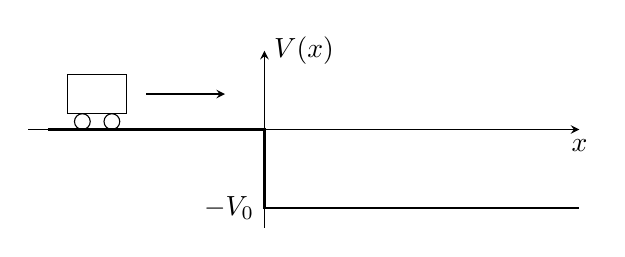
\begin{tikzpicture}
\pgfmathsetmacro{\ka}{0.75}
\pgfmathsetmacro{\kb}{0.5}
\pgfmathsetmacro{\r}{0.1}
%\draw[help lines, thick,gray,step=1] (0,0) grid (12,12);
\draw[-stealth] (-3,0) -- (4,0) node[below]{$x$};
\draw[-stealth] (0,-1.25) -- (0,1) node[right]{$V(x)$};
\draw[thick] (-2.75,0)--(0,0)--(0,-1)node[left]{$-V_0$}--(4,-1);
\draw[](-2.5,2*\r)--++(\ka,0)coordinate[pos=0.25](wa)coordinate[pos=0.75](wb)--++(0,\kb)coordinate[pos=0.5](pa)--++(-\ka,0)--++(0,-\kb) ;
\draw(wa)++(0,-\r) circle (\r);
\draw(wb)++(0,-\r) circle (\r);
\draw[-stealth] (pa)++(0.25,0)--++(1,0);
\end{tikzpicture}
\caption{عمودی چٹان سے بکھراو (سوال \حوالہ{سوال_غیر_تابع_اچانک_گہرائی})۔}
\label{شکل_غیر_تابع_شروڈنگر_عمودی_چٹان_بکھراو}
\end{figure}
%
\begin{enumerate}[a.]
\item
 صورت\عددی{ E=V_{0}/3 }  میں اس کے انعکاس کا احتمال کیا ہو گا؟ \ترچھا{ اشارہ:} یہ بالکل سوال \حوالہ{سوال_شروڈنگر_سیڑھی_رکاوٹ} کی طرح ہے، بس یہاں سیڑھی اوپر کی بجائے نیچے کو ہے ۔
\item 
 میں نے مخفیہ کی شکل و صورت یوں پیش کی ہے گویا ایک گاڑی افقی چٹان سے نیچے گرنے والی ہے تاہم ایسی کھائی سے گاڑی کا ٹکرا کر واپس لوٹنے کا احتمال جزو -ا کے نتیجہ سے بہت کم ہو گا ۔یہ مخفیہ کیوں ایک افقی چٹان کی صحیح ترجمانی نہیں کرتا ہے؟ \ترچھا{ اشارہ:} شکل \حوالہ{شکل_غیر_تابع_شروڈنگر_عمودی_چٹان_بکھراو} میں جیسے ہی گاڑی نقطہ \عددی{ x=0} پر سے گزرتی ہے ، اس کی توانائی عدم استمرار کے ساتھ گر کر\عددی{-V_{0}} ہو جاتی ہے؛ کیا یہ نیچے گرتے ہوئی گاڑی کے لیے درست ہو گا ؟
\item
ایک نیوٹران مرکزہ میں داخل ہوتے ہوئے مخفیہ میں اچانک کمی محسوس کرتا ہے۔ باہر \عددی{V=0} جبکہ مرکزہ کے اندر \عددی{V=\SI{-12}{\mega\electronvolt}} ہو تا ہے۔ فرض کریں بذریعہ انشقاق خارج ایک نیوٹران جس کی حرکی توانائی \عددی{\SI{4}{\mega\electronvolt}} ہو ایک ایسے مرکزہ کو ٹکراتا ہے۔ اس نیوٹران کا جذب ہو کر دوسرا انشقاق پیدا کرنے کا احتمال کیا ہو گا؟ \ترچھا{اشارہ:} آپ نے جزو-ا میں انعکاس کا احتمال تلاش کیا؛ کلیہ \عددی{T=1-R} استعمال کر کے سطح سے ترسیل کا احتمال حاصل کریں۔
\end{enumerate}
\انتہا{سوال}

\جزوحصہء{مزید سوالات برائے باب \حوالہ{باب_غیر_تابع_وقت_شروڈنگر_مساوات}}
\ابتدا{سوال}\شناخت{سوال_غیر_تابع_مبدا_پر_مرکز}
عین مبدا پر \عددی{-a< x< +a} کے بیچ لامتناہی چوکور کنویں  کے اندر\عددی{ V(x)=0 } اور اس کے باہر\عددی{ V(x)=\infty} ہے ۔ غیر تابع وقت شروڈنگر مساوات پر موزوں سرحدی شرائط مسلط کر کے اسے حل کریں۔ تصدیق کریں کہ آپ کی توانائیاں عین میری حاصل کردہ توانائیوں (مساوات\حوالہ{مساوات_شروڈنگر_لامتناہی_چکور_کنواں_توانائیاں}) کے مطابق ہیں  اور تصدیق کریں کہ میری \عددی{ \psi} (مساوات \حوالہ{مساوات_شروڈنگر_میری_سائے}) میں \عددی{ x\to (x+a)/2 } پر کر کے، موزوں معمول زنی سے آپ کی تمام \عددی{\psi} حاصل ہوتی ہیں۔ اپنے اولین تین حل ترسیم کریں اور ان کا موازنہ شکل \حوالہ{شکل_غیر_تابع_لامتناہی_چکور_تین_ساکن_حالات} سے کریں۔ دھیان رہے کہ یہاں کنویں  کی چوڑائی \عددی{ 2a} ہے ۔ 
\انتہا{سوال}
\ابتدا{سوال}
 لامتناہی چوکور کنویں ( مساوات \حوالہ{مساوات_شروڈنگر_لامتناہی_چکور}) میں ایک ذرے کا ابتدائی تفاعل موج درج ذیل ہے۔
 \begin{align*}
 \Psi(x,0)&=A\sin^{3}(\pi x/a) && (0\le x\le a)
\end{align*}

 مستقل\عددی{ A} اور \عددی{ \Psi(x,t)} تلاش کر کے وقت کے لحاظ سے \عددی{\langle x \rangle} کا حساب لگائیں۔ توانائی کی توقعاتی قیمت کیا ہو گی؟ \ترچھا{ اشارہ :} \عددی{\sin^n\theta} اور \عددی{ \cos^n\theta} کو تخفیف کے بعد\عددی{\sin(m\theta)} اور \عددی{\cos(m\theta)}کے خطی جوڑ لکھا جا سکتا ہے جہاں \عددی{ m=0,1,2,\dotsc ,n } ہو گا۔
\انتہا{سوال}
\ابتدا{سوال}
 کمیت\عددی{ m} کا ایک ذرہ لامتناہی چوکور کنویں  ( مساوات \حوالہ{مساوات_شروڈنگر_لامتناہی_چکور}) میں زمینی حال میں ہے ۔ اچانک کنویں کا دایاں دیوار \عددی{ a } سے \عددی{ 2a} منتقل ہوتا ہے جس سے کنویں  کی چوڑائی دگنی ہو جاتی ہے۔ لمحاتی طور پر اس عمل سے تفاعل موج اثر انداز نہیں ہوتا۔ اس ذرہ کی توانائی کی پیمائش اب کی جاتی ہے۔
\begin{enumerate}[a.]
\item
 کونسا نتیجہ سب سے زیادہ امکان رکھتا ہے؟ اس نتیجے کے حصول کا احتمال کیا ہو گا؟ 
\item
 کونسا نتیجہ اس کے بعد زیادہ امکان رکھتا ہے اور اس کا احتمال کیا ہو گا؟
\item 
توانائی کی توقعاتی قیمت کیا ہو گی؟ \ترچھا{ اشارہ:} اگر آپ کو لامتناہی تسلسل کا سامنا ہو تب کوئی دوسری ترکیب استعمال کریں۔
\end{enumerate} 
 \انتہا{سوال}
\ابتدا{سوال}
\begin{enumerate}[a.]
\item 
 دکھائیں کہ لامتناہی چوکور کنویں  میں ایک ذرہ کا تفاعل موج کوانٹائی\اصطلاح{ تجدیدی عرصہ}\فرہنگ{تجدیدی عرصہ}\حاشیہب{revival time}\فرہنگ{revival time} \عددی{T=4ma^{2}/\pi \hslash } کے بعد دوبارہ اپنے اصل روپ میں واپس آتا ہے۔ یعنی ( نہ صرف ساکن حال ) بلکہ کسی بھی حال کے لئے \عددی{ \Psi(x,T)=\Psi(x,0)} ہوتا ہے۔ 
\item 
 دیواروں سے ٹکرا کر دائیں سے بائیں اور بائیں سے دائیں حرکت کرتے ہوئے ایک ذرہ جس کی توانائی \عددی{ E} ہو کا کلاسیکی تجدیدی عرصہ کیا ہو گا ؟ 
\item 
 کس توانائی کیلئے یہ تجدیدی عرصے ایک دوسرے کے برابر ہوں گے؟\حاشیہد{یہ  غور طلب تضاد ہے کہ کلاسیکی اور کوانٹائی تجدیدی عرصوں کا بظاہر ایک دوسرے کے ساتھ کوئی تعلق نہیں پایا جاتا ہے (اور کوانٹائی تجدیدی عرصہ توانائی پر منحصر بھی نہیں ہے۔)}
\end{enumerate} 
\انتہا{سوال}
%86
\ابتدا{سوال}
 ایک ذرہ جس کی کمیت \عددی{ m } ہے درج ذیل مخفی کو میں پایا جاتا ہے۔ 
\begin{align*}
V(x)=
\begin{cases}
\infty & (x< 0)\\
-32\hslash^{2}/ma^{2} & (0\le x \le a)\\
0 & (x> a)
\end{cases}
\end{align*}

\begin{enumerate}[a.]
\item
 اس کے مقید حلوں کی تعداد کیا ہو گی ؟
\item 
 مقید حال میں سب سے زیادہ توانائی کی صورت میں کنویں  کے باہر (\عددی{ x> a}) ذرہ پائے جانے کا احتمال کیا ہو گا ؟
\ترچھا{جواب:} \عددی{ 0.542 }، اگرچہ یہ کنویں  میں مقید ہے، تاہم اس کا کنویں  سے باہر پائے جانے کا امکان زیادہ ہے۔ 
\end{enumerate}
\انتہا{سوال}
\ابتدا{سوال}
ایک ذرہ جس کی کمیت\عددی{m} ہے ہارمونی مرتعش کی مخفیہ (مساوات \حوالہ{مساوات_شروڈنگر_مخفیہ_ہارمونی}) میں درج ذیل حال سے آغاز کرتا ہے جہاں\عددی{A} کوئی مستقل ہے۔
\begin{align*}
\Psi(x,0)=A\Big(1-2\sqrt{\frac{m\omega}{\hslash}}\, x \Big)^{2}e^{-\frac{m\omega}{2\hslash}x^{2}}
\end{align*}
%
\begin{enumerate}[a.]
\item
 توانائی کی توقعاتی قیمت کیا ہے ؟
\item
مستقبل کے لمحہ \عددی{T} پر تفاعل موج درج ذیل ہو گا
\begin{align*}
\Psi(x,T)=B\Big(1+2\sqrt{\frac{m\omega}{\hslash}}\,x \Big)^{2}e^{-\frac{m\omega}{2\hslash}x^{2}} 
\end{align*}
 جہاں \عددی{ B } کوئی مستقل ہے۔ لمحہ \عددی{ T } کی کم سے کم ممکنہ قیمت کیا ہو گی؟ 
\end{enumerate}
\انتہا{سوال}
\ابتدا{سوال}
درج ذیل نصف ہارمونی مرتعش کی اجازتی توانائیاں تلاش کریں۔
\begin{align*}
V(x)=
\begin{cases}
(1/2)m\omega^{2}x^{2}&x> 0\\
\infty & x< 0
\end{cases}
 \end{align*}
(مثلاً ایک ایسا اسپرنگ جس کو کھینچا تو جا سکتا ہے لیکن دبایا نہیں جا سکتا ہے۔) \ترچھا{اشارہ:} اس کو حل کرنے کے لئے آپ کو ایک بار اچھی طرح مغز ماری کرنی  ہو گی جبکہ حقیقی حساب بہت کم درکار ہو گی۔ 
\انتہا{سوال}
\ابتدا{سوال}\شناخت{سوال_شروڈنگر_ساکن_گاوسی_آزاد_ذرہ_موجی_اکٹھ}
آپ نے سوال \حوالہ{سوال_شروڈنگر_گاوسی_موجی_اکٹھ} میں ساکن گاوسی آزاد ذرہ موجی اکٹھ کا تجزیہ کیا۔ اب ابتدائی تفاعل موج 
\begin{align*}
\Psi(x,0)=Ae^{-ax^{2}}e^{ilx} 
\end{align*} 
 جہاں \عددی{ l}ایک حقیقی مستقل ہے سے آغاز کرتے ہوئے متحرک گاوسی موجی اکٹھ کے لیے یہی مسئلہ دوبارہ حل کریں۔
\انتہا{سوال}
\ابتدا{سوال}
مبدا پر لامتناہی چوکور کنواں، جس کے وسط پر درج ذیل ڈیلٹا تفاعل رکاوٹ ہو، کے لیے غیر تابع وقت شروڈنگر مساوات حل کریں۔
\begin{align*}
V(x)=
\begin{cases}
\alpha\delta (x)& -a< x< +a\\
\infty &\abs{x}\ge a
\end{cases}
 \end{align*} 
 جفت اور طاق تفاعل امواج کو علیحدہ علیحدہ حل کریں ۔انہیں معمول پر لانے کی ضرورت نہیں ہے ۔ اجازتی توانائیوں کو ( اگر ضرورت پیش آئے) ترسیمی طور پر تلاش کریں۔ ان کا موازنہ ڈیلٹا تفاعل کی غیر موجودگی میں مطابقتی توانائیوں کے ساتھ کریں۔ طاق حلوں پر ڈیلٹا تفاعل کا کوئی اثر نہ ہونے پر تبصرہ کریں ۔ تحدیدی صورتیں \عددی{ a\to 0 } اور \عددی{ a\to \infty}پر تبصرہ کریں۔ 
\انتہا{سوال}
\ابتدا{سوال}\شناخت{سوال_شروڈنگر_یکبعدی_منفرد_نا_ممکن}
 ایسے دو یا دو سے زیادہ غیر تابع وقت شروڈنگر مساوات کے منفرد\حاشیہد{ایسے دو حل جن میں صرف جزو ضربی کا فرق پایا جاتا ہو (جن میں ایک مرتبہ معمول پر لانے کے بعد صرف دوری جزو \عددی{e^{i\phi}} کا فرق پایا جاتا ہو) درحقیقت ایک ہی حل کو ظاہر کرتے ہیں لہٰذا انہیں یہاں منفرد نہیں کہا جا سکتا ہے۔یہاں "منفرد" سے مراد "خطی طور پر غیر تابع" ہے۔} حل جن کی توانائی \عددی{ E} ایک  جیسی ہو کو \اصطلاح{ انحطاطی}\فرہنگ{انحطاطی}\حاشیہب{degenerate}\فرہنگ{degenerate} کہتے ہیں۔ مثال کے طور پر آزاد ذرہ کے حال دوہری انحطاطی ہیں۔ ان میں سے ایک حل دائیں رخ اور دوسرا بائیں رخ حرکت کو ظاہر کرتا ہے ۔ تاہم ہم نے ایسے کوئی انحطاطی حل نہیں دیکھے جو معمول پر لانے کے قابل ہوں اور یہ محض ایک اتفاق نہیں ہے۔ 
 درج ذیل مسئلہ ثابت کریں : 
\ترچھا{یک بعدی مقید انحطاطی حال نہیں پائے جاتے ہیں۔}\حاشیہد{جیسا ہم باب \حوالہ{باب_تین_ابعادی_کوانٹم_میکانیات} میں دیکھیں گے، بلند ابعاد میں ایسی انحطاط عام پائی جاتی ہیں۔فرض کریں کہ مخفیہ علیحدہ علیحدہ حصوں پر مشتمل نہیں ہے جن کے بیچ خطہ میں \عددی{V=\infty} ہو۔ مثلاً دو تنہا لامتناہی کنویں مقید انحطاطی حال دیں گے جہاں ذرہ ایک یا دوسرے کنویں  میں پایا جائے گا۔} 
\ترچھا{اشارہ:} فرض کریں
\عددی{ \psi_{1} } اور \عددی{ \psi_{2} } ایسے دو حل ہوں جن کی توانائی، \عددی{ E}، ایک  جیسی ہو ۔ حل \عددی{ \psi_{1} } کی شروڈنگر مساوات کو \عددی{ \psi_{2} } سے ضرب دیں اور اس سے \عددی{ \psi_{2} }کی شروڈنگر مساوات کو \عددی{ \psi_{1} } سے ضرب دے کر منفی کر کے دکھائیں کہ \عددی{\psi_{2}\dif{\psi_{1}}/\dif{x}- \psi_{1}\dif{\psi_{2}}/\dif{x}} ایک مستقل ہو گا۔
 اب \عددی{\pm \infty} پر  معمول پر لائے جانے کے قابل ہر حل \عددی{\psi\to 0} ہو گا۔ اس حقیقت کو استعمال کرتے ہوئے دکھائیں کہ یہ مستقل در حقیقت صفر ہو گا جس سے آپ نتیجہ اخذ کر سکتے ہیں کہ \عددی{\psi_{2}} دراصل \عددی{\psi_{1}} کا مضرب ہے لہٰذا یہ حل دو الگ الگ حل نہیں ہو سکتے ہیں ۔
\انتہا{سوال}
\ابتدا{سوال}\شناخت{سوال_غیر_تابع_شروڈنگر_بے_رگڑ_موتی}
فرض کریں کمیت \عددی{ m} کا ایک موتی ایک دائری چھلا پر بے رگڑ حرکت کرتا ہے۔ چھلے کا محیط \عددی{ L} ہے ۔ (یہ ایک آزاد ذرہ کی مانند ہے تاہم یہاں\عددی{ \psi(x+L)=\psi(x) } ہو گا۔) اس کے ساکن حال تلاش کر کے انہیں معمول پر لائیں اور ان کی مطابقتی اجازتی توانائیاں دریافت کریں ۔ آپ دیکھیں گے کہ ہر ایک توانائی\عددی{E_{n}} کے لئے دو آپس میں غیر تابع حل پائے جائیں گے جن میں سے ایک گھڑی وار اور دوسرا خلاف گھڑی حرکت کے لیے ہو گا، جنہیں آپ\عددی{ \psi_{n}^{+}(x) } اور \عددی{ \psi_{n}^{-}(x) } کہہ سکتے ہیں۔سوال \حوالہ{سوال_شروڈنگر_یکبعدی_منفرد_نا_ممکن} کے مسئلہ کو مد نظر رکھتے ہوئے آپ اس انحطاط کے بارے میں کیا کہیں گے (اور یہ مسئلہ یہاں کارآمد کیوں نہیں ہے)؟ 
\انتہا{سوال}

%============
%prob 2.47

\ابتدا{سوال}\شناخت{سوال_غیر_تابع_شروڈنگر_موین_دہرا_کنواں}
آپ کو صرف کیفی تجزیہ کی اجازت ہے حساب کرکے نتیجہ اخذ کرنے کی اجازت نہیں ہے۔شکل \حوالہ{شکل_غیر_تابع_شروڈنگر_دوہرا_چکور_کنواں}میں دکھائے گئے  " دوہرا چوکور کنواں" پر غور کریں جہاں گہرائی \عددی{V_0} اور چوڑائی \عددی{a} مقررہ ہیں جو اتنے بڑے ضرور ہیں کہ کئی مقید حال ممکن ہوں۔

%fig 2.21 pg 100
\begin{figure}
\centering
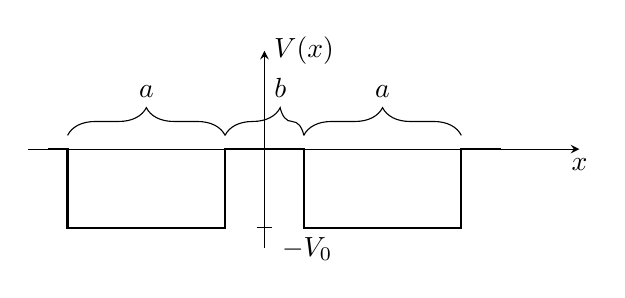
\begin{tikzpicture}
\pgfmathsetmacro{\ka}{0.75}
\pgfmathsetmacro{\kb}{0.5}
%\draw[help lines, thick,gray,step=1] (0,0) grid (12,12);
\draw[-stealth] (-3,0) -- (4,0) node[below]{$x$};
\draw[-stealth] (0,-1.25) -- (0,1.25) node[right]{$V(x)$};
\draw[thick](-2.75,0)--(-2.5,0)--(-2.5,-1)--(-0.5,-1)--(-0.5,0)--(0.5,0)--(0.5,-1)--(2.5,-1)--(2.5,0)--(3,0);
\draw(-0.1,-1)--(0.1,-1)node[below right]{$-V_0$};
\draw[decorate,decoration={brace,amplitude=10pt,raise=5pt}](-2.5,0)--(-0.5,0)node[pos=0.5,above,yshift=1.5em]{$a$};
\draw[decorate,decoration={brace,amplitude=10pt,raise=5pt}](0.5,0)--(2.5,0)node[pos=0.5,above,yshift=1.5em]{$a$};
\draw[decorate,decoration={brace,amplitude=10pt,raise=5pt,aspect=0.7}](-0.5,0)--(0.5,0)node[pos=0.7,above,yshift=1.5em]{$b$};
\end{tikzpicture}
\caption{دوہرا چوکور کنواں (سوال \حوالہ{سوال_غیر_تابع_شروڈنگر_موین_دہرا_کنواں})۔}
\label{شکل_غیر_تابع_شروڈنگر_دوہرا_چکور_کنواں}
\end{figure}


\begin{enumerate}[a.]
\item
زمینی تفاعل موج \عددی{\psi_1} اور پہلا ہیجان حال \عددی{\psi_2} کا خاکہ درج ذیل صورت میں کھینچیں۔
\begin{multicols}{3}
\begin{enumerate}[1.]
\item
 \عددی{b=0}،
 \item
 \عددی{b\approx a}،
\item 
  \عددی{b\gg a}
 \end{enumerate}
 \end{multicols}
\item
 \عددی{b} کی قیمت صفر سے لامتناہی تک بڑھتے ہوئے مطابقتی توانائیاں (\عددی{E_1} اور \عددی{E_2}) کس طرح تبدیل ہوتی ہیں، اس کا کیفی جواب دیں۔ \عددی{E_1(b)} اور \عددی{E_2(b)} کو ایک ساتھ ترسیم کریں۔
\item
 دو جوہری سالمہ میں الیکٹران پر اثر انداز مخفی توانائی کا تاریخی یک دوری نمونہ دوہرا کنواں پیش کرتا ہے ( مرکزوں کی قوت کشش کو دو کنویں ظاہر کرتی ہیں)۔ اگر مراکزے آزادی سے حرکت کر سکتے ہوں تب یہ کم سے کم توانائی تشکیل  اختیار کریں گے۔ جزو-(ب میں حاصل نتائج کے تحت کیا الیکٹران ان مرکزوں کو ایک دوسرے کے قریب کھینچے گا یا انہیں ایک دوسرے سے دور رہنے پر مجبور کرے گا۔( اگرچہ دو مرکزوں کے بیچ قوت دفع بھی پایا جاتا ہے تاہم اس کی بات یہاں نہیں کی جا رہی ہے۔)
\end{enumerate}
\انتہا{سوال}
\ابتدا{سوال}\شناخت{سوال_غیر_تابع_ترکیب_کی_وضاحت}
آپ نے مساوات \حوالہ{مساوات_غیر_تابع_وقت_توانائی_توقعاتی_قیمت} کے تسلسل کا مجموعہ لیتے ہوئے سوال \حوالہ{سوال_غیر_تابع_شروڈنگر_ابتدائی_تفاعل_موج_چکور_کنواں}-د میں توانائی کی توقعاتی قیمت تلاش کی جہاں حاشیہ میں آپ کو میں نے آگاہ کیا کہ اس کو \عددی{\langle H \rangle=\int\psi(x, 0)^*H\psi(x, 0)\dif x} کے  پرانے طریقہ سے حاصل نہ کریں چونکہ \عددی{\psi(x, 0)} کے پہلے تفرق میں عدم استمرار دوسرے تفرق کو پریشان کن بناتا ہے۔ حقیقت میں آپ تکمل بالحصص کے ذریعے اسے حل کر سکتے تھے لیکن ڈیراک ڈیلٹا تفاعل اس طرح کے انوکھا مسائل حل کرنے کا ایک بہترین طریقہ فراہم کرتا ہے۔
\begin{enumerate}[a.]
\item
 آپ سوال \حوالہ{سوال_غیر_تابع_شروڈنگر_ابتدائی_تفاعل_موج_چکور_کنواں} میں \عددی{\psi(x, 0)} کا پہلا تفرق حاصل کر کے اس کو سیڑھی تفاعل \عددی{\theta(x-a/2)} کی صورت میں لکھیں جسے مساوات \حوالہ{مساوات_غیر_تابع_شروڈنگر_تھیٹا_سیڑھی_تفاعل} میں پیش کیا گیا ہے۔( آخری سروں کی فکر نہ کریں، صرف اندرونی خطہ \عددی{0<x<a} کے لیے لکھیں۔)
\item
 ابتدائی موجی تفاعل \عددی{\psi(x, 0)} کے دوہرا تفرق کو سوال \حوالہ{سوال_شروڈنگر_تفاعلات_برابر}-ب کا نتیجہ استعمال کرتے ہوئے ڈیلٹا تفاعل کی صورت میں لکھیں۔
\item
 تکمل \عددی{\int\psi(x, 0)^*H\psi(x, 0)\dif x} کو حل کرکے اس کی قیمت حاصل کر کے تصدیق کریں کہ یہ وہی نتیجہ ہے جو آپ پہلے حاصل کر چکے ہیں۔
\end{enumerate}
\انتہا{سوال}
\ابتدا{سوال}\شناخت{سوال_غیر_تابع_وقت_بعد_لمبائی}
\begin{enumerate}[a.]
\item
 دکھائیں کہ ہارمونی مرتعش کی مخفی توانائی ( مساوات \حوالہ{مساوات_شروڈنگر_مخفیہ_ہارمونی}) کے لئے
\begin{align*}
	\psi(x, t)=\left(\frac{m\omega}{\pi\hslash}\right)^{1/4}e^{-\frac{m\omega}{2\hslash}\left(x^2+\frac{a^2}{2}(1+e^{-2i\omega t})+\frac{i\hslash t}{m}-2axe^{-i\omega t}\right)}
\end{align*}
  تابع وقت شروڈنگر مساوات پر پورا اترتا ہے جہاں \عددی{a} ایک حقیقی مستقل ہے جس کا بُعد لمبائی ہے۔\حاشیہد{تابع وقت شروڈنگر مساوات کے ٹھیک ٹھیک بند روپ میں حل کی یہ ایک نایاب مثال ہے۔}
\item
 \عددی{\abs{\psi(x, t)}^2} تلاش کریں اور موجی اکٹھ کی حرکت پر تبصرہ کریں۔
\item
 \عددی{\langle x \rangle} اور \عددی{\langle p \rangle} کا حساب لگائیں اور دیکھیں آیا مسئلہ اہرنفسٹ  (مساوات \حوالہ{مساوات_تفاعل_موج_مخفی_توانائی_سے_معیار_حرکت})  پر یہ پورا اترتے ہیں۔
\end{enumerate}
\انتہا{سوال}
\ابتدا{سوال}\شناخت{سوال_غیر_تابع_حرکت_پذیر_کنواں}
درج ذیل حرکت کرتے ہوئے ڈیلٹا تفاعل کنویں  پر غور کریں 
\begin{align*}
	V(x, t)=-\alpha\delta(x-v t)
\end{align*}
جہاں  کنویں  کی (غیر تغیر) سمتی رفتار کو  \عددی{v} ظاہر کرتا ہے۔
\begin{enumerate}[a.]
\item
 دکھائیں کہ تابع وقت شروڈنگر مساوات کا حل درج ذیل ہے
\begin{align*}
	\psi(x, t)=\frac{\sqrt{m\alpha}}{\hslash}e^{-m\alpha\abs{x-v t}/\hslash^2}e^{-i[(E+(1/2)m v^2)t-m v x]/\hslash}
\end{align*}
جہاں \عددی{E=-m\alpha^2/2\hslash^2} ساکن ڈیلٹا تفاعل کے مقید حال کی توانائی ہے۔ اشارہ: اس حل کو شروڈنگر مساوات میں پُر کر کے آپ تصدیق کر سکتے ہیں ۔سوال \حوالہ{سوال_شروڈنگر_تفاعلات_برابر}-ب کا نتیجہ استعمال کریں۔
\item
 اس حال میں ہیملٹنی کی توقعاتی قیمت تلاش کر کے نتیجے پر تبصرہ کریں۔
\end{enumerate}
\انتہا{سوال}
\ابتدا{سوال}
درج ذیل مخفیہ پر غور کریں 
\begin{align*}
	V(x)=-\frac{\hslash^2a^2}{m}\operatorname{sech}^2(ax)
\end{align*}
جہاں \عددی{a} ایک مثبت مستقل ہے۔
\begin{enumerate}[a.]
\item
 اس مخفیہ کو ترسیم کریں۔
\item
تصدیق کریں کہ اس مخفیہ کا زمینی حال درج ذیل ہے
\begin{align*}
	\psi_0(x)=A\operatorname{sech}(ax)
\end{align*}
اور اسکی توانائی تلاش کریں۔ \عددی{\psi_0} کو معمول پر لا کر اس کی ترسیم کا خاکہ بنائیں۔
\item
دکھائیں کہ درج ذیل تفاعل کسی بھی (مثبت) توانائی \عددی{E} کے لیے شروڈنگر مساوات کو حل کرتا ہے (جہاں ہمیشہ کی طرح \عددی{k\equiv\sqrt{2mE}/\hslash} ہے)۔
\begin{align*}
	\psi_k(x)=A\left(\frac{ik-a\tanh(ax)}{ik+a}\right)e^{ikx}
\end{align*}
 چونکہ \عددی{z\to-\infty} کرنے سے \عددی{\tanh z\to -1} ہوگا لہٰذا \عددی{x} کی بہت بڑی منفی قیمتوں کے لیے درج ذیل ہو گا 
\begin{align*}
	\psi_k(x)\approx Ae^{ikx}\quad \text{\RL{کے لیے}}x\text{\RL{بڑی منفی}}
\end{align*}
جو \عددی{e^{-ikx}} کی عدم موجودگی کی بنا، بائیں سے آمد ایک موج کو ظاہر کرتا ہے جس میں کوئی انعکاسی موج نہیں پائی جاتی ہے۔ \عددی{x} کی بڑی مثبت قیمتوں کے لیے \عددی{\psi_k(x)} کی متقاربی روپ  کیا ہوگی؟ اس مخفیہ کے لیے \عددی{R} اور \عددی{T} کیا ہوں گے؟ \ترچھا{تبصرہ:} یہ \موٹا{بلا انعکاس مخفیہ }\فرہنگ{مخفیہ!بلاانعکاس}\حاشیہب{reflectionless potential}\فرہنگ{potential!reflectionless}کی ایک بہت مشہور مثال ہے؛ ہر ذرہ، اس سے قطع نظر کہ اس کی توانائی کتنی ہے، اس مخفیہ سے سیدھا گزرتا ہے۔
\end{enumerate}
\انتہا{سوال}
\ابتدا{سوال}\شناخت{سوال_غیر_تابع_شروڈنگر_قالب_بکھراو}
\موٹا{قالب بکھراو۔}\فرہنگ{قالب!بکھراو}\حاشیہب{scattering matrix}\فرہنگ{scattering!matrix} مقامی مخفیہ کے لیے بکھراو کا نظریہ ایک عمومی صورت اختیار کرتا ہے (شکل \حوالہ{شکل_غیر-تابع_شروڈنگر_اختیاری_مقامی-مخفیہ})۔ بائیں ہاتھ خطہ-ا  میں \عددی{V(x)=0} ہے لہٰذا درج ذیل ہوگا۔
\begin{align}
	\psi(x)=Ae^{ikx}+Be^{-ikx},&& k\equiv\frac{\sqrt{2mE}}{\hslash}\text{\RL{جہاں}}
\end{align}
دائیں ہاتھ خطہ-ج میں بھی \عددی{V(x)=0} ہے لہٰذا یہاں درج ذیل ہوگا
\begin{align}
	\psi(x)=Fe^{ikx}+Ge^{-ikx}
\end{align}
%fig 2.22 pg 102
\begin{figure}
\centering
\begin{tikzpicture}
\pgfmathsetmacro{\ka}{0.75}
\pgfmathsetmacro{\kb}{0.5}
%\draw[help lines, thick,gray,step=1] (0,0) grid (12,12);
\draw[-stealth] (-3,0) -- (4,0) node[below]{$x$};
\draw[-stealth] (0,-0.5) -- (0,1.5) node[left]{$V(x)$};
\draw[thick](-3,0)--(-1.25,0) to [out=0,in=180](-0.75,0.5) to [out=0,in=180](-0.25,0.25) to [out=0,in=180](0.5,1) to [out=0,in=180](1.25,-0.5) to [out=0,in=180](1.75,0.25) to [out=0,in=180](2.5,0)--(3.75,0);
\draw[-stealth](-3,1.5)--++(1,0)node[pos=0.5,above]{$Ae^{ikx}$};
\draw[stealth-](-3,1)--++(1,0)node[pos=0.5,below]{$Be^{-ikx}$};
\draw[stealth-](4,1.5)--++(-1,0)node[pos=0.5,above]{$Fe^{ikx}$};
\draw[-stealth](4,1)--++(-1,0)node[pos=0.5,below]{$Ge^{-ikx}$};
\draw[decorate,decoration={brace,amplitude=10pt,mirror}](-3,-0.5)--(-1.3,-0.5)node[pos=0.5,below,yshift=-1em]{\RL{خطہ-ا}};
\draw[decorate,decoration={brace,amplitude=10pt,mirror}](-1.25,-0.5)--(2.5,-0.5)node[pos=0.5,below,yshift=-1em]{\RL{خطہ-ب}};
\draw[decorate,decoration={brace,amplitude=10pt,mirror}](2.6,-0.5)--(3.75,-0.5)node[pos=0.5,below,yshift=-1em]{\RL{خطہ-ج}};
\end{tikzpicture}
\caption{مقامی اختیاری مخفیہ (جو خطہ-2 کے علاوہ \عددی{V(x)=0} ہے) سے بکھراو (سوال \حوالہ{سوال_غیر_تابع_شروڈنگر_قالب_بکھراو})۔}
\label{شکل_غیر-تابع_شروڈنگر_اختیاری_مقامی-مخفیہ}
\end{figure}
%
ان دونوں کے بیچ خطہ-ب میں مخفیہ جانے بغیر میں آپ کو \عددی{\psi} کے بارے میں کچھ نہیں بتا سکتا، تاہم چونکہ شروڈنگر مساوات خطی اور دو رتبی تفرقی ہے لہٰذا اس کا عمومی حل لازماً درج ذیل روپ کا ہوگا
\begin{align*}
	\psi(x)=Cf(x)+Dg(x)
\end{align*}
جہاں \عددی{f(x)} اور \عددی{g(x)} دو خطی غیر تابع مخصوص حل ہیں۔ یہاں چار عدد سرحدی شرائط ہوں گے جن میں سے دو خطہ-ا  اور ب کو جوڑیں گے اور باقی دو خطہ-ب اور ج کو جوڑیں گے۔ ان میں سے دو کو استعمال کر کے \عددی{C} اور \عددی{D} کو خارج کرتے ہوئے باقی دو کو حل کر کے \عددی{A} اور \عددی{G} کی صورت میں \عددی{B} اور \عددی{F} تلاش کیے جا سکتے ہیں:
\begin{align*}
	B=S_{11}A+S_{12}G,&& F=S_{21}A+S_{22}G
\end{align*}
یہ چار عددی سر \عددی{S_{ij}} جو \عددی{k} (لہٰذا \عددی{E})  پر منحصر ہیں \عددی{2\times2} قالب ٍ\عددی{\mat{S}} دیتے ہیں جس کو \اصطلاح{ قالب بکھراو}\فرہنگ{قالب!بکھراو}\حاشیہب{scattering matrix}\فرہنگ{scattering!matrix} یا مختصراً \اصطلاح{قالب \عددی{\mat{S}} }\حاشیہب{S-matrix}\فرہنگ{matrix!S} کہتے ہیں۔ قالب \عددی{S} آپ کو آمدی حیطوں (\عددی{A} اور \عددی{G}) کی صورت میں رخصتی حیطوں (\عددی{B} اور \عددی{F}) کی قیمت دیتا ہے:
\begin{align}\label{مساوات_غیر_تابع_شروڈنگر_قالب_بکھراو_بی_ایف}
	\begin{pmatrix}
		B\\
		F
	\end{pmatrix}
	=
	\begin{pmatrix}
		S_{11} & S_{12}\\
		S_{21} & S_{22}
	\end{pmatrix}
	\begin{pmatrix}
		A\\
		G
	\end{pmatrix}
\end{align}
بائیں سے بکھراو کی صورت میں \عددی{G=0} ہوگا لہٰذا انعکاسی اور ترسیلی شرح درج ذیل ہوں گی۔
\begin{align}\label{مساوات_غیر_تابع_شروڈنگر_آر_ایس}
	R_l=\frac{\abs{B}^2}{\abs{A}^2}\bigg|_{G=0}=\abs{S_{11}}^2,&& T_l=\frac{\abs{F}^2}{\abs{A}^2}\bigg|_{G=0}=\abs{S_{21}}^2
\end{align}
دائیں سے بکھراو کی صورت میں \عددی{A=0} ہوگا لہٰذا درج ذیل ہوں گے۔
\begin{align}\label{مساوات_غیر_تابع_شروڈنگر_آر_ٹی}
	R_r=\frac{\abs{F}^2}{\abs{G}^2}\bigg|_{A=0}=\abs{S_{22}}^2,&& T_r=\frac{\abs{B}^2}{\abs{G}^2}\bigg|_{A=0}=\abs{S_{12}}^2
\end{align}
%
\begin{enumerate}[a.]
\item
 ڈیلٹا تفاعل کنویں  (مساوات \حوالہ{مساوات_شروڈنگر_کنواں_مخفیہ}) کے لیے بکھراو کا قالب  \عددی{S} تیار کریں۔
\item
 لامتناہی چوکور کنویں  (مساوات \حوالہ{مساوات_شروڈنگر_متناہی_چکور_کنواں_مخفیہ}) کے لیے قالب \عددی{S} تیار کریں۔ \ترچھا{اشارہ:} مسئلہ کی تشاکلی پن بروئے  کار لائیں۔ نئے کام کی ضرورت نہیں ہوگی۔ 
\end{enumerate}
\انتہا{سوال}
\ابتدا{سوال}\شناخت{سوال_غیر_تابع_شروڈنگر_دو_تنہا}
\موٹا{قالب ترسیل۔}\فرہنگ{قالب!ترسیل}\حاشیہب{transfer matrix}\فرہنگ{matrix!transfer} قالب \عددی{S}( سوال \حوالہ{سوال_غیر_تابع_شروڈنگر_قالب_بکھراو})  آپ کو رخصتی حیطوں ( \عددی{B} اور \عددی{F}) کو آمدی حیطوں (\عددی{A} اور \عددی{G}) کی صورت میں پیش کرتا ہے (مساوات \حوالہ{مساوات_غیر_تابع_شروڈنگر_قالب_بکھراو_بی_ایف})۔ بعض اوقات ترسیلی قالب \عددی{M} کے ساتھ کام کرنا زیادہ آسان ثابت ہوتا ہے جو مخفیہ کے دائیں جانب حیطوں (\عددی{F} اور \عددی{G}) کو بائیں جانب حیطوں (\عددی{A} اور \عددی{B}) کی صورت میں پیش کرتا ہے:
\begin{align}
	\begin{pmatrix}
		F\\
		G
	\end{pmatrix}
	=
	\begin{pmatrix}
		M_{11} & M_{12} \\
		m_{21} & M_{22}
	\end{pmatrix}
	\begin{pmatrix}
		A\\
		B
	\end{pmatrix}
\end{align}
%
\begin{figure}
\centering
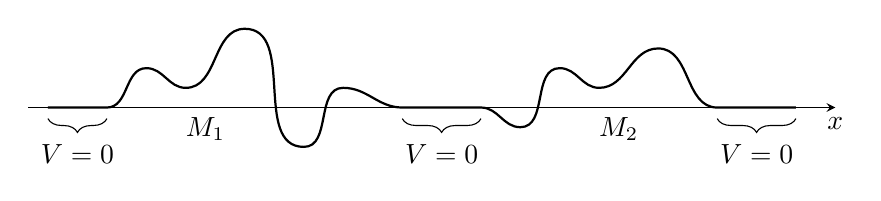
\begin{tikzpicture}
\draw[-stealth] (-2.25,0) -- (8,0) node[below]{$x$};
\draw[thick](-2,0)--(-1.25,0) to [out=0,in=180](-0.75,0.5) to [out=0,in=180](-0.25,0.25) to [out=0,in=180](0.5,1) to [out=0,in=180](1.25,-0.5) to [out=0,in=180](1.75,0.25) to [out=0,in=180](2.5,0)--(3.5,0)
to [out=0,in=180]++(0.5,-0.25) to [out=0,in=180]++(0.5,0.75) to [out=0,in=180]++(0.5,-0.25) to [out=0,in=180]++(0.75,0.5) to [out=0,in=180]++(0.75,-0.75)--++(1,0);
\draw[decorate,decoration={brace,amplitude=5pt,raise=4pt,mirror}](-2,0)--(-1.25,0)node[pos=0.5,below,yshift=-1em]{$V=0$};
\draw[decorate,decoration={brace,amplitude=5pt,raise=4pt,mirror}](2.5,0)--(3.5,0)node[pos=0.5,below,yshift=-1em]{$V=0$};
\draw[decorate,decoration={brace,amplitude=5pt,raise=4pt,mirror}](6.5,0)--(7.5,0)node[pos=0.5,below,yshift=-1em]{$V=0$};
\draw(0,0)node[below]{$M_1$};
\draw(5.25,0)node[below]{$M_2$};
\end{tikzpicture}
\caption{دو تنہا حصوں پر مبنی مخفیہ (سوال \حوالہ{سوال_غیر_تابع_شروڈنگر_دو_تنہا})۔}
\label{شکل_غیر_تابع_شروڈنگر_دو_تنہا_مخفیہ}
\end{figure}
%
\begin{enumerate}[a.]
\item
قالب \عددی{S} کے اجزاء کی صورت میں قالب \عددی{M} کے چار اجزاء تلاش کریں۔ اسی طرح قالب \عددی{M} کے چار اجزاء کی صورت میں قالب \عددی{S} کے اجزاء تلاش کریں۔ مساوات \حوالہ{مساوات_غیر_تابع_شروڈنگر_آر_ایس} اور مساوات \حوالہ{مساوات_غیر_تابع_شروڈنگر_آر_ٹی} میں دیے گئے \عددی{R_l, T_l, R_r} اور \عددی{T_r} کو \عددی{\mat{M}} قالب کے ارکان کی صورت میں لکھیں۔
\item
فرض کریں آپ کے پاس ایک ایسا مخفیہ ہو جو دو تنہا ٹکڑوں پر مشتمل ہو (شکل \حوالہ{شکل_غیر_تابع_شروڈنگر_دو_تنہا_مخفیہ})۔ دکھائیں کہ اس پورے نظام کا \عددی{M} قالب ان دو حصوں کے انفرادی \عددی{M} قالب کا حاصل ضرب ہوگا۔
\begin{align}
	\mat{M}=\mat{M}_2\mat{M}_1
\end{align}
(ظاہر ہے کے آپ دو سے زیادہ عدد انفرادی مخفیہ بھی استعمال کر سکتے تھے۔ یہی \عددی{M} قالب کی اہمیت کا سبب ہے۔)
\item
 نقطہ \عددی{a} پر (درج ذیل) واحد ایک ڈیلٹا تفاعل مخفیہ سے بکھراو کا \عددی{M} قالب تلاش کریں۔
\begin{align*}
	V(x)=-\alpha\delta(x-a)
\end{align*}
\item
 جزو-ب کا طریقہ استعمال کرتے ہوئے دوہرا ڈیلٹا تفاعل
\begin{align*}
	V(x)=-\alpha[\delta(x+a)+\delta(x-a)]
\end{align*}
کے لیے \عددی{M} قالب تلاش کریں۔ اس مخفیہ کی ترسیلی شرح کیا ہوگی؟
\end{enumerate}
\انتہا{سوال}
\ابتدا{سوال}\شناخت{سوال_غیر_تابع_شروڈنگر_دم_ہلانا}
\اصطلاح{دم ہلانے}\فرہنگ{دم ہلانا} کی ترکیب سے ہارمونی مرتعش کی زمینی حال توانائیوں کو پانچ معنی خیز ہندسوں تک تلاش کریں۔ یعنی \عددی{K} کو تبدیل کرتے ہوئے مساوات \حوالہ{مساوات_شروڈنگر_تحلیلی_شروڈنگر} کو اعدادی طریقہ سے یوں حل کریں کہ \عددی{\xi} کی بڑی قیمت کے لیے حاصل تفاعل موج صفر تک پہنچنے کی کوشش کرے۔ ماتھیمٹیکا میں درج ذیل پُر کرنے سے ایسا ہوگا
\begin{gather*}
\begin{aligned}
	\text{Plot}[\text{Evaluate}[u[x]/.\text{NDSolve}[{u''[x]-(x^2-K)^*u[x]==0, u[0]==1, u'[0]==0},\\
	u[x],{x, 10^{-8}, 10}, \text{MaxSteps}->\num{10000}]], {x, a, b}, \text{PlotRange}->{c, d}]
\end{aligned}
\end{gather*}
یہاں \عددی{a, b} ترسیم کی افقی سعت  جبکہ \عددی{c, d} انتصابی سعت ہے(ابتدا \عددی{a=0}، \عددی{b=10}،\عددی{c=-10} اور \عددی{d=10} سے کریں)۔ ہم جانتے ہیں کہ اس کا درست جواب \عددی{K=1} ہے لہٰذا آپ \عددی{K=0.9} سے شروع کر سکتے ہیں۔ تفاعل موج کی "دم" پر نظر رکھیں۔ اب \عددی{K=1.1} لیں، آپ دیکھیں گے کہ دم دوسری طرف پلٹ جائے گی۔ ان دونوں کے بیچ کہیں درست حل موجود ہے۔ \عددی{K} کی قیمت کو درست قیمت کے دونوں اطراف قریب سے قریب لانے سے درست جواب حاصل ہوگا۔
\انتہا{سوال}
\ابتدا{سوال}
دم ہلانے کا طریقہ (سوال \حوالہ{سوال_غیر_تابع_شروڈنگر_دم_ہلانا}) استعمال کرتے ہوئے ہارمونی مرتعش کے ہیجان حال توانائی کو پانچ با معنی ہندسوں تک تلاش کریں۔ پہلی اور تیسری ہیجان حال کے لیے آپ کو \عددی{u[0]==0} اور \عددی{u'[0]==1} لینا ہوگا۔
\انتہا{سوال}
\ابتدا{سوال}\شناخت{سوال_غیر_تابع_وقت_دم_ہلانا_آخری}
دم ہلانے کی ترکیب سے لامتناہی چوکور کنویں  کی اولین چار توانائیوں کی قیمتیں پانچ با معنی ہندسوں تک تلاش کریں۔ اشارہ: سوال \حوالہ{سوال_غیر_تابع_شروڈنگر_دم_ہلانا}  کی تفرقی مساوات میں درکار تبدیلیاں لائیں۔ اس بار آپ کو \عددی{u(1)=0}چاہتے ہیں۔
\انتہا{سوال}

